% Options for packages loaded elsewhere
\PassOptionsToPackage{unicode}{hyperref}
\PassOptionsToPackage{hyphens}{url}
%
\documentclass[
  table]{report}
\usepackage{amsmath,amssymb}
\usepackage{iftex}
\ifPDFTeX
  \usepackage[T1]{fontenc}
  \usepackage[utf8]{inputenc}
  \usepackage{textcomp} % provide euro and other symbols
\else % if luatex or xetex
  \usepackage{unicode-math} % this also loads fontspec
  \defaultfontfeatures{Scale=MatchLowercase}
  \defaultfontfeatures[\rmfamily]{Ligatures=TeX,Scale=1}
\fi
\usepackage{lmodern}
\ifPDFTeX\else
  % xetex/luatex font selection
\fi
% Use upquote if available, for straight quotes in verbatim environments
\IfFileExists{upquote.sty}{\usepackage{upquote}}{}
\IfFileExists{microtype.sty}{% use microtype if available
  \usepackage[]{microtype}
  \UseMicrotypeSet[protrusion]{basicmath} % disable protrusion for tt fonts
}{}
\makeatletter
\@ifundefined{KOMAClassName}{% if non-KOMA class
  \IfFileExists{parskip.sty}{%
    \usepackage{parskip}
  }{% else
    \setlength{\parindent}{0pt}
    \setlength{\parskip}{6pt plus 2pt minus 1pt}}
}{% if KOMA class
  \KOMAoptions{parskip=half}}
\makeatother
\usepackage{xcolor}
\usepackage{graphicx}
\makeatletter
\def\maxwidth{\ifdim\Gin@nat@width>\linewidth\linewidth\else\Gin@nat@width\fi}
\def\maxheight{\ifdim\Gin@nat@height>\textheight\textheight\else\Gin@nat@height\fi}
\makeatother
% Scale images if necessary, so that they will not overflow the page
% margins by default, and it is still possible to overwrite the defaults
% using explicit options in \includegraphics[width, height, ...]{}
\setkeys{Gin}{width=\maxwidth,height=\maxheight,keepaspectratio}
% Set default figure placement to htbp
\makeatletter
\def\fps@figure{htbp}
\makeatother
\setlength{\emergencystretch}{3em} % prevent overfull lines
\providecommand{\tightlist}{%
  \setlength{\itemsep}{0pt}\setlength{\parskip}{0pt}}
\setcounter{secnumdepth}{5}
\AtBeginDocument{\let\maketitle\relax}
\usepackage{lastpage} % Calculate the last page of the document
\usepackage{tocbibind} % Insert custom table of content items
\usepackage{graphicx} % import figure
\graphicspath{{figures/}}
\usepackage{float} % Allow for more granular control of float of figures
\floatplacement{figure}{H}
\usepackage{setspace}
\usepackage{lipsum} % Generate lorem ipsum text
\usepackage[fontsize=12pt]{scrextend}
\usepackage{fontspec} % change to system font
\usepackage{tcolorbox} % Fancy text boxes that are pretty
\tcbset{ definitionstyle/.style={ colback=orange!5!white, colframe=orange!80!black, top=0.25cm, bottom=0.25cm, before=\vspace{0.5cm}, after=\vspace{0.5cm} } }
\usepackage{todonotes}
\usepackage[style=apa, natbib=true]{biblatex}
\addbibresource{nebula_refs.bib}
\addbibresource{manual-nebula.bib}
\DefineBibliographyExtras{english}{}
\usepackage{minted}
\usemintedstyle{xcode}
\usepackage{csquotes}
\usepackage{hyperref}
\usepackage{cleveref}
\usepackage{booktabs}
\usepackage{array}
\onehalfspacing
\usepackage[a4paper,width=150mm,top=25mm,bottom=25mm]{geometry}
\usepackage{fancyhdr}
\pagestyle{fancy}
\fancyhf{}
\fancyfoot[C]{}
\usepackage[bottom]{footmisc}
\tcbuselibrary{theorems}
\renewcommand{\headrulewidth}{0pt}
\renewcommand{\arraystretch}{1.7} % Adjust the value as needed
\usepackage{epigraph}
\setlength\epigraphwidth{.6\textwidth}
\setmainfont{Georgia}
\usepackage{titlesec}
\newfontfamily\headingfont{Avenir}
\titleformat{\chapter}[display]{\headingfont\large}{\chaptertitlename\ \thechapter}{20pt}{\Huge}
\titleformat*{\section}{\Large\headingfont}
\titleformat*{\subsection}{\large\headingfont}
\titleformat*{\subsubsection}{\large\headingfont}
\hyphenation{Web-Assembly}
\usepackage{acronym}
\usepackage{booktabs}
\usepackage{longtable}
\usepackage{array}
\usepackage{multirow}
\usepackage{wrapfig}
\usepackage{float}
\usepackage{colortbl}
\usepackage{pdflscape}
\usepackage{tabu}
\usepackage{threeparttable}
\usepackage{threeparttablex}
\usepackage[normalem]{ulem}
\usepackage{makecell}
\usepackage{xcolor}
\ifLuaTeX
  \usepackage{selnolig}  % disable illegal ligatures
\fi
\usepackage[]{biblatex}
\usepackage{bookmark}
\IfFileExists{xurl.sty}{\usepackage{xurl}}{} % add URL line breaks if available
\urlstyle{same}
\hypersetup{
  pdftitle={Nebula},
  pdfauthor={Marius Nilsen Kluften},
  hidelinks,
  pdfcreator={LaTeX via pandoc}}

\title{Nebula}
\usepackage{etoolbox}
\makeatletter
\providecommand{\subtitle}[1]{% add subtitle to \maketitle
  \apptocmd{\@title}{\par {\large #1 \par}}{}{}
}
\makeatother
\subtitle{Comparing two waves of cloud computing}
\author{Marius Nilsen Kluften}
\date{2024}

\begin{document}
\maketitle

\begin{titlepage}
\thispagestyle{fancy}
\fancyfoot[C]{2024}
\centering
{\Huge\bfseries Nebula\par}

\vspace{0.5cm}

{\Huge\itshape Comparing two waves of cloud compute\par}

\vspace{1cm}

{\Large Marius Nilsen Kluften\par}

\vspace{1cm}


\includegraphics[width=0.4\textwidth]{assets/uio-logo.png}\\[1cm]

{\Large Thesis submitted for the degree of\par}
{\Large Master in Informatics: Programming and System Architecture\par}

\vspace{0.25cm}

{\Large 60 credits\par}

\vspace{1cm}

{\Large Institute of Informatics\par}

{\Large Faculty of mathematics and natural sciences\par}

{\Large University of Oslo\par}

\end{titlepage}

\newpage

\begin{center}
\vspace*{\fill} 
\Huge \textbf{Nebula} \\[10pt]
\vspace{2cm} 
\Large \textit{Comparing two waves of cloud compute} \\[20pt]
\vspace{2cm} 
\Large Marius Nilsen Kluften \\[30pt]
\vspace*{\fill} 
\end{center}

\newpage
\listoftodos
\newpage

\null\vfill
\begin{flushleft}
\Large © 2024 Marius Nilsen Kluften\par
\Large Nebula \par
\Large https://duo.uio.no/ \par
\Large Printed: Reprosentralen, University of Oslo \par
\end{flushleft}

\newpage
\fancyfoot[C]{ \thepage\ }
\pagenumbering{roman}

\vspace*{\fill}
\begin{center}
\begin{minipage}{0.75\textwidth}

\addcontentsline{toc}{chapter}{Abstract}
\chapter*{Abstract}

The ever increasing demand for cloud services has resulted in the expansion of
energy-intensive data centers, the ICT industry accounts for about 1 \% of global 
electricity use, highlighting a need for sustainable options
in cloud computing architectures.

\vspace{0.25cm}

This thesis investigates WebAssembly, a technology originally intended for running 
in the browser, as a potential contender in the space of technologies to
consider in cloud native applications. Leveraging the inherent efficiency,
portability and lower startup times of WebAssembly modules, this thesis presents an
approach that aligns with green energy principles, while maintaining performance and
scalability, essential for cloud services. 

\vspace{0.25cm}

Preliminary findings suggest that programs compiled to WebAssembly modules have
reduced startup and runtimes, which hopefully leads to lower energy consumption,
offering a viable pathway towards more sustainable cloud computing.

\end{minipage}
\end{center}
\vspace*{\fill}

\newpage

\vspace*{\fill}
\begin{center}
\begin{minipage}{0.75\textwidth}

\addcontentsline{toc}{chapter}{Acknowledgements}
\chapter*{Acknowledgments}

The idea for the topic for this thesis appeared in an episode of the podcast
"Rustacean station". Matt Butcher, the CEO of Fermyon, told the story of his
journey through the different waves of cloud computing, and how Fermyon was
founded as a software company that aimed to build a cloud platform with
WebAssembly and lead the charge into the next big wave of cloud compute.

\vspace{0.25cm}

The capabilities of WebAssembly running on the server, with the aid of the
WebAssembly System Interface project, caught my interest and started the
snowball that ended up as the avalanche that is this thesis. I would like to
thank Matt Butcher and the people over at Fermyon for inadvertently inspiring my
topic. 

\vspace{0.25cm}

I would also like to thank my two supervisors Joachim Tilsted Kristensen and 
Michael Kirkedal Thomsen, whom I somehow managed to convinced to help guide me 
through such a cutting edge topic. Their guidance and insight have been
invaluable the past semesters. 

\vspace{0.25cm}

Finally, I would like to thank Syrus Akbary, founder of Wasmer. If I hadn't met
him at the WasmIO 2024 conference in Barcelona, my startup times would be 100
times slower.

\end{minipage}
\end{center}
\vspace*{\fill}

\newpage

\tableofcontents

\newpage

\listoffigures

\newpage

\listoftables

\newpage

\pagenumbering{arabic}

\part{Overview}

\newpage

\chapter{Introduction}
\label{chap:intro}

\epigraph{\itshape 
  If WASM+WASI existed in 2008, we wouldn't have needed to created Docker. 
  That's how important it is. Webassembly on the server is the future of computing.
  A standardized system interface was the missing link. 
  Let's hope WASI is up to the task!
}{---Solomon Hykes, \textit{Founder of Docker}}

In the digital age, cloud computing has emerged as a foundational
technology in the technological landscape, driving innovation and
increased efficiency across various sectors. Its growth over the past
decade has not only transformed how consumers store, process, and access
data, but it has also raised environmental concerns as more and more
data centers are built around the globe to accommodate the traffic,
consuming vast amounts of power. The Information and Communication
Technology (ICT) industry, with cloud computing at its core, accounts
for an estimated 2.1\% to 3.9\% of global greenhouse gas emissions. Data
centers, the backbone of cloud computing infrastructures, are
responsible for about 200 TWh/yr, or about 1\% of the global electricity
consumption, a figure projected to escalate, potentially reaching 15\%
to 30\% of electricity consumption in some countries by 2030
\citep{freitag2021}.

The sustainability of cloud computing is thus under scrutiny, and while
some vendors strive to achieve a net-zero carbon footprint for their
cloud computing services, many data centers still rely on electricity
generated by fossil fuels, a leading contributor to climate change
\citep{mytton2020}. This reality emphasizes an urgent need to explore
alternative technologies that promise enhanced energy efficiency while
meeting customers demands. In this vein, serverless computing has
emerged as a compelling paradigm, offering scalability and flexibility
by enabling functions to execute in response to requests, rather than
having a server running all the time. However, the inherent startup
latency associated with containerized serverless functions pose a
challenge, particularly for on-demand applications. To mitigate this,
vendors often opt for keeping the underlying servers \emph{warm} to keep
the startup latency as low as possible for serving functions. Reducing
the startup time for serving a function should reduce the need for
keeping servers warm and therefore reduce the standby power consumption
of serverless architectures.

\section{Motivation}
\label{sect:motivation}

The environmental footprint of cloud computing, particularly the energy
demands of data centers, is a pressing issue.~As the digital landscape
continues to evolve, the quest for sustainable solutions has never been
more critical. This thesis is motivated by the need to reconcile the
growing demand for cloud services with the pressing need for
environmental sustainability. Through the lens of WebAssembly and
\ac{WASI}, this thesis aims to investigate innovative deployment methods
that promise to reduce energy consumption without sacrificing
performance, thereby contributing to the development of a more
sustainable cloud computing ecosystem.

\section{The Project}
\label{sect:project}

This thesis explores \ac{Wasm} with \ac{WASI} as an innovative choice
for deploying functions to the cloud, through developing a prototype
\ac{FaaS} platform named Nebula. This platform will run functions
compiled to \ac{Wasm}, originally designed for high-performance tasks in
web browsers, which coupled with \ac{WASI}, allows us to give
WebAssembly programs access to the underlying system. This holds
potential for a more efficient way to package and deploy functions,
potentially reducing the startup latency and the overhead associated
with traditional serverless platforms. \ac{Wasm} and \ac{WASI} offers a
pathway, where the demands of today is met, while reducing the carbon
footprint for cloud applications.

\section{Problem Statement}
\label{sect:problems}

The goal of the thesis is to:

\begin{enumerate}
\def\labelenumi{\arabic{enumi}.}
\tightlist
\item
  Develop a prototype cloud computing platform for the \ac{FaaS}
  paradigm.
\item
  Use this platform for conducting experiments that either prove or
  disprove the claim that WebAssembly is the more efficient choice.
\item
  Determine whether or not WebAssembly is a more energy efficient
  choice.
\end{enumerate}

By achieving these goals this thesis seeks to shed light on the
feasibility and implications of adopting \ac{Wasm} and \ac{WASI} for a
greener cloud.

\section{Outline}

The thesis has five chapters; this introduction, a chapter that goes
through the background for how cloud computing got to this point, a
chapter dedicated to the process of building Nebula, a chapter for
discussing the results from the experiments, and ending with a chapter
suggesting future works.

\todo[inline=true]{Feedback from Michael: When I write this, use it to point the reader to
the most important parts of the thesis. Avoid listing the chapters; you already
have a table-of-contents.}

\newpage

\chapter{Three waves of cloud compute}
\label{chap:three-waves}

\setlength\epigraphwidth{.35\textwidth}

\epigraph{\itshape 
The most dangerous phrase in the language is `We\'ve always done it this way`"
}{Grace Hopper}

The evolution of cloud computing represents a transformative adventure,
driven by the pursuit for efficiency, scalability and reliability, yet
it also poses challenges, notably its environmental impact. This chapter
steps introduces the concept of the ``Three waves of cloud computing'',
coined by the WebAssembly community
\citep*{butcherDodds2024, leonardWebAssemblyHeraldsThird2024}. Where the
two first waves of cloud compute represent the shift from virtual
machines to containerization, the third wave encompasses utilizing
\ac{Wasm} and \ac{WASI} to build the next era of cloud compute with the
potential to significantly reduce the carbon footprint.

\section{Ashore: Before the Waves}
\label{sect:ashore}

Before delving into the waves themselves, it is useful to understand the
landscape that preceded cloud computing. Prior to the cloud era,
companies were required to building and mantaining the physical
infrastructure for their digital services in-house. This required
companies to invest heavily into both expensive hardware and expensive
engineers to buy, upkeep and oversee their own physical servers and
network hardware. (See \Cref{fig:myspeis} for an example)

\begin{figure}[H]
\centering
  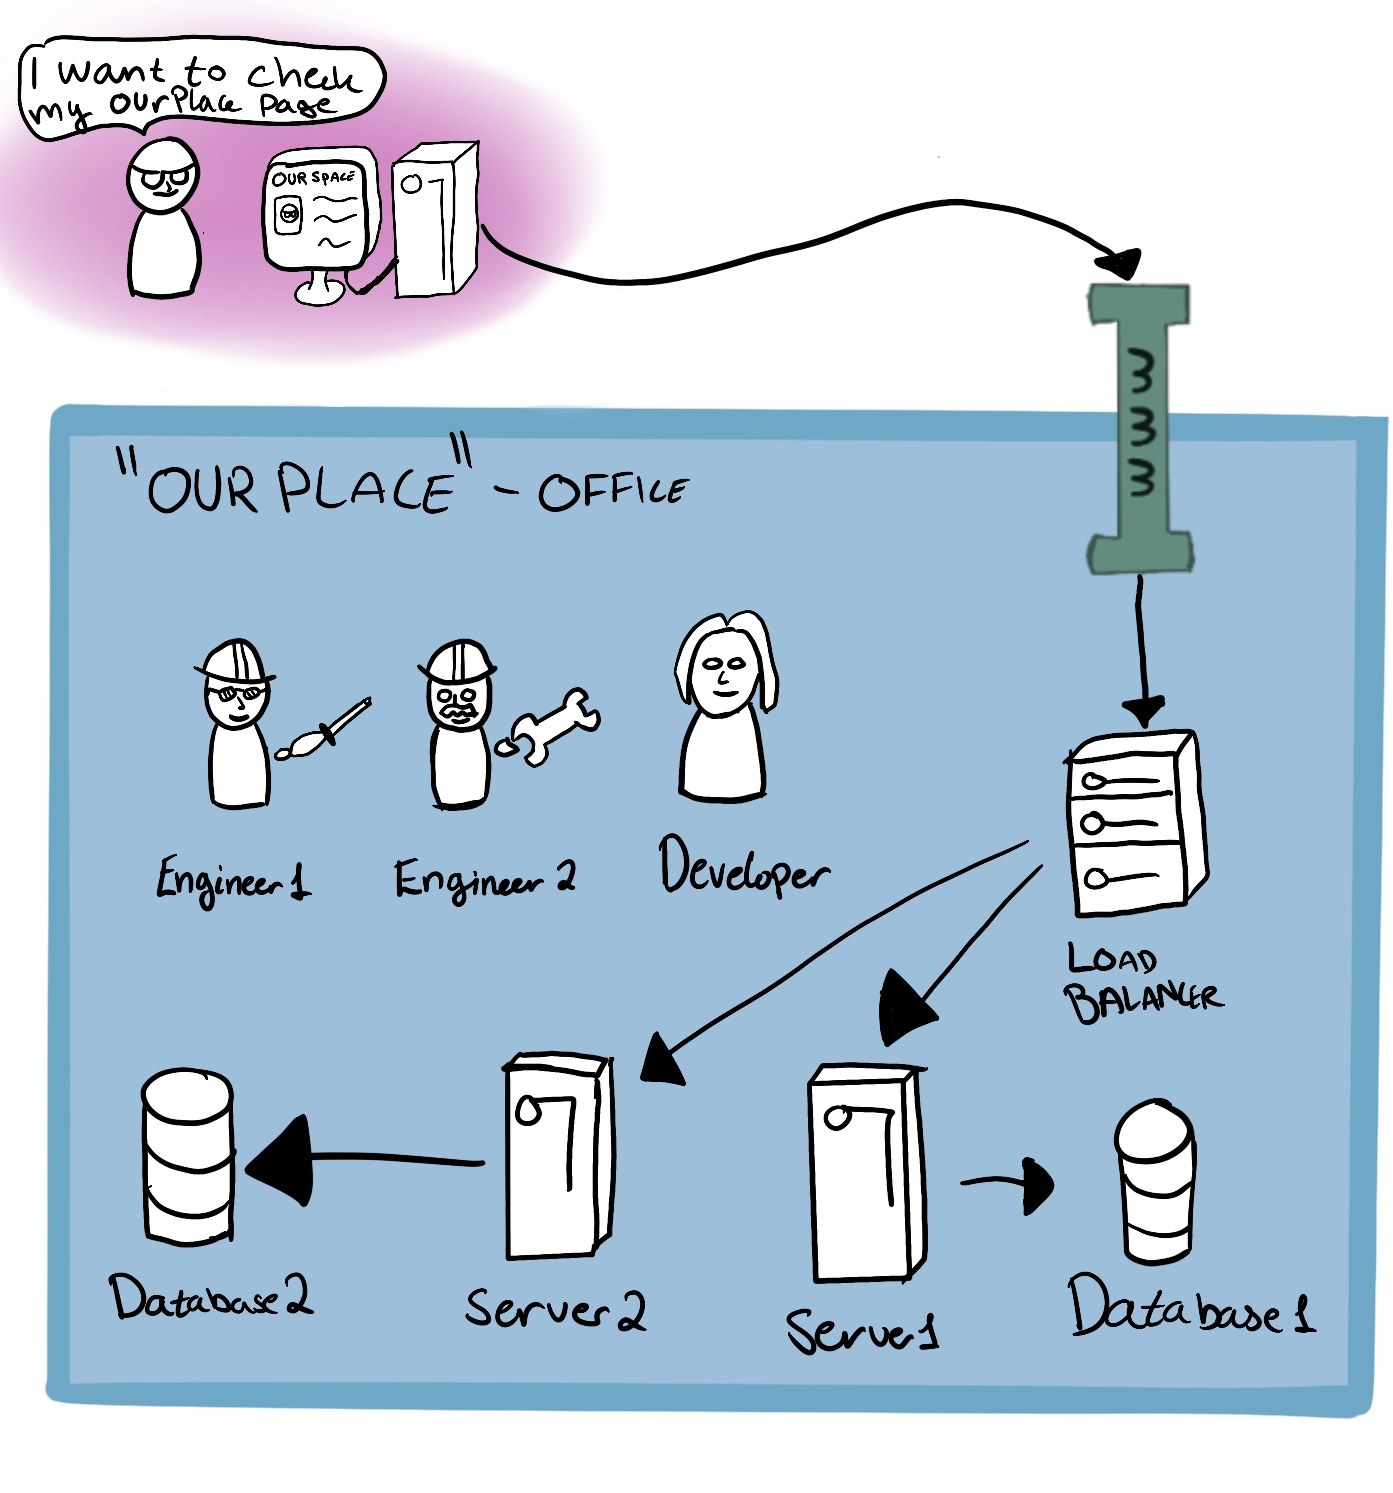
\includegraphics[width=0.7\columnwidth]{assets/pre-wave.jpg}
  \caption{Example of a company that host their own infrastructure.}
  \label{fig:myspeis}
\end{figure}

Setting up such an infrastructure comes with a significant cost, both
upfront for purchasing such a setup and for employing engineers who can
set up and maintain this. This puts a considerable financial strain on
organizations, and kept smaller companies without the financial backing
to invest in this at a disadvantage \citep{etroEconomicImpactCloud2009}.
Having to maintain infrastructure also poses a challenge when the
services start to gain traction. To meet the increased traffic on the
services, a company will have to scale up and extend the infrastructure,
which also can be expensive and difficult
\citep{armbrustViewCloudComputing2010}.

As a response to these challenges, some companies found a market for
taking on the responsibility of managing infrastructure, and offer
\ac{IaaS} to an evolving market that relies more and more on digital
solutions. \ac{IaaS} provides consumers with the ability to provision
computing resources where they can deploy and run software, including
operating systems and applications \citep{nist-def}. On these managed
infrastructures companies could deploy their services on top of virtual
machines that allowed more flexibility, and lowered the bar to new
companies.

\section{The First Wave: Virtual machines}
\label{sect:first-wave}

The start of cloud computing can be traced back to the emergence of
virtualization, more specifically virtual machines, a response to the
costly and complex nature of managing traditional, on-premise data
centers. During the mid-2000s, Amazon launched its subsidiary, \ac{AWS},
who in turn launched Amazon S3 in March 2006, followed by Elastic
Compute Cloud (EC2) in August the same year
\citep{barrAmazonEC2Beta2006}. With these services, \ac{AWS} positioned
itself as a pioneer in this space, marking a major turning point in
application development and deployment, and popularized cloud computing.
EC2, as an \ac{IaaS} platform, empowered developers to run virtual
machines remotely. (See \Cref{fig:feisbook} for an example of this kind
of architecture)

\begin{figure}[H]
\centering
  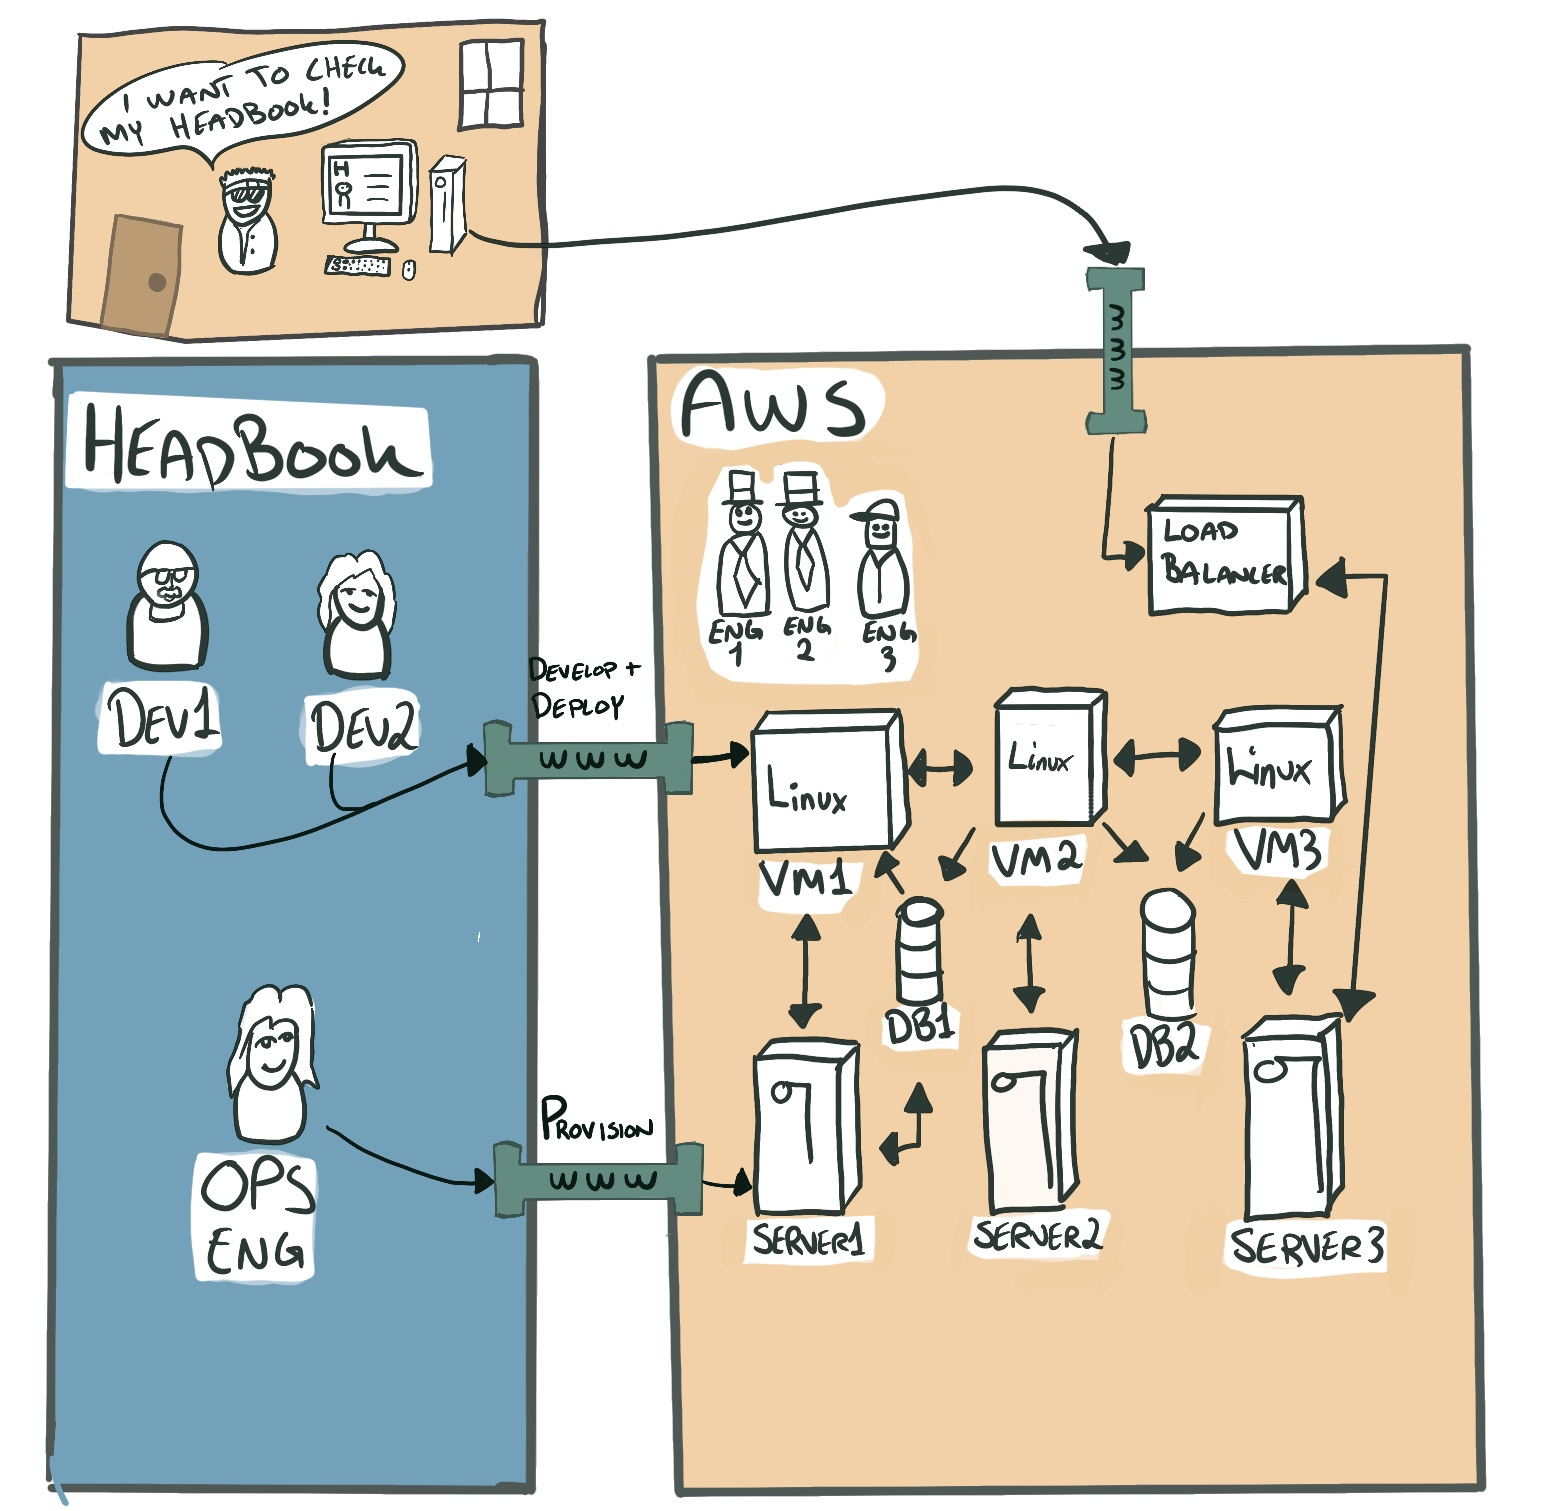
\includegraphics[width=0.7\columnwidth]{assets/aws-wave.jpg}
  \caption{Example of ``Fæisbook`` building their services on EC2 and using S3
for storage.}
  \label{fig:feisbook}
\end{figure}

While similar services existed before 2006, with Amazon's existing large
customer base helped them gain significant traction, and ushered in a
the first era, or wave, of \emph{cloud computing}.

\section{The Second Wave: Containers}
\label{sect:second-wave}

As we entered the 2010s, the focus shifted from virtual machines to
containers, largely due to the limitations of VMs in efficiency,
resource utilization, and application deployment speed. Containers,
being a lightweight alternative to VMs, designed to overcome these
hurdles \citep{bao2016}.

In contrast to VMs, which require installation of resource-intensive
operating systems and minutes to start up, containers along with their
required OS components, could start up in seconds. Typically managed by
orchestration tools like Kubernetes\footnote{\url{https://kubernetes.io}},
containers enabled applications to package alongside their required OS
components, facilitating scalability in response to varying service
loads. Consequently, an increasing number of companies have since
established platform teams to build orchestrated developers platforms,
thereby simplifying application development in Kubernetes clusters. (See
\Cref{fig:docker} for an example where a fictive company
\texttt{WacDonalds} and their container workflow)

\begin{figure}[H]
\centering
  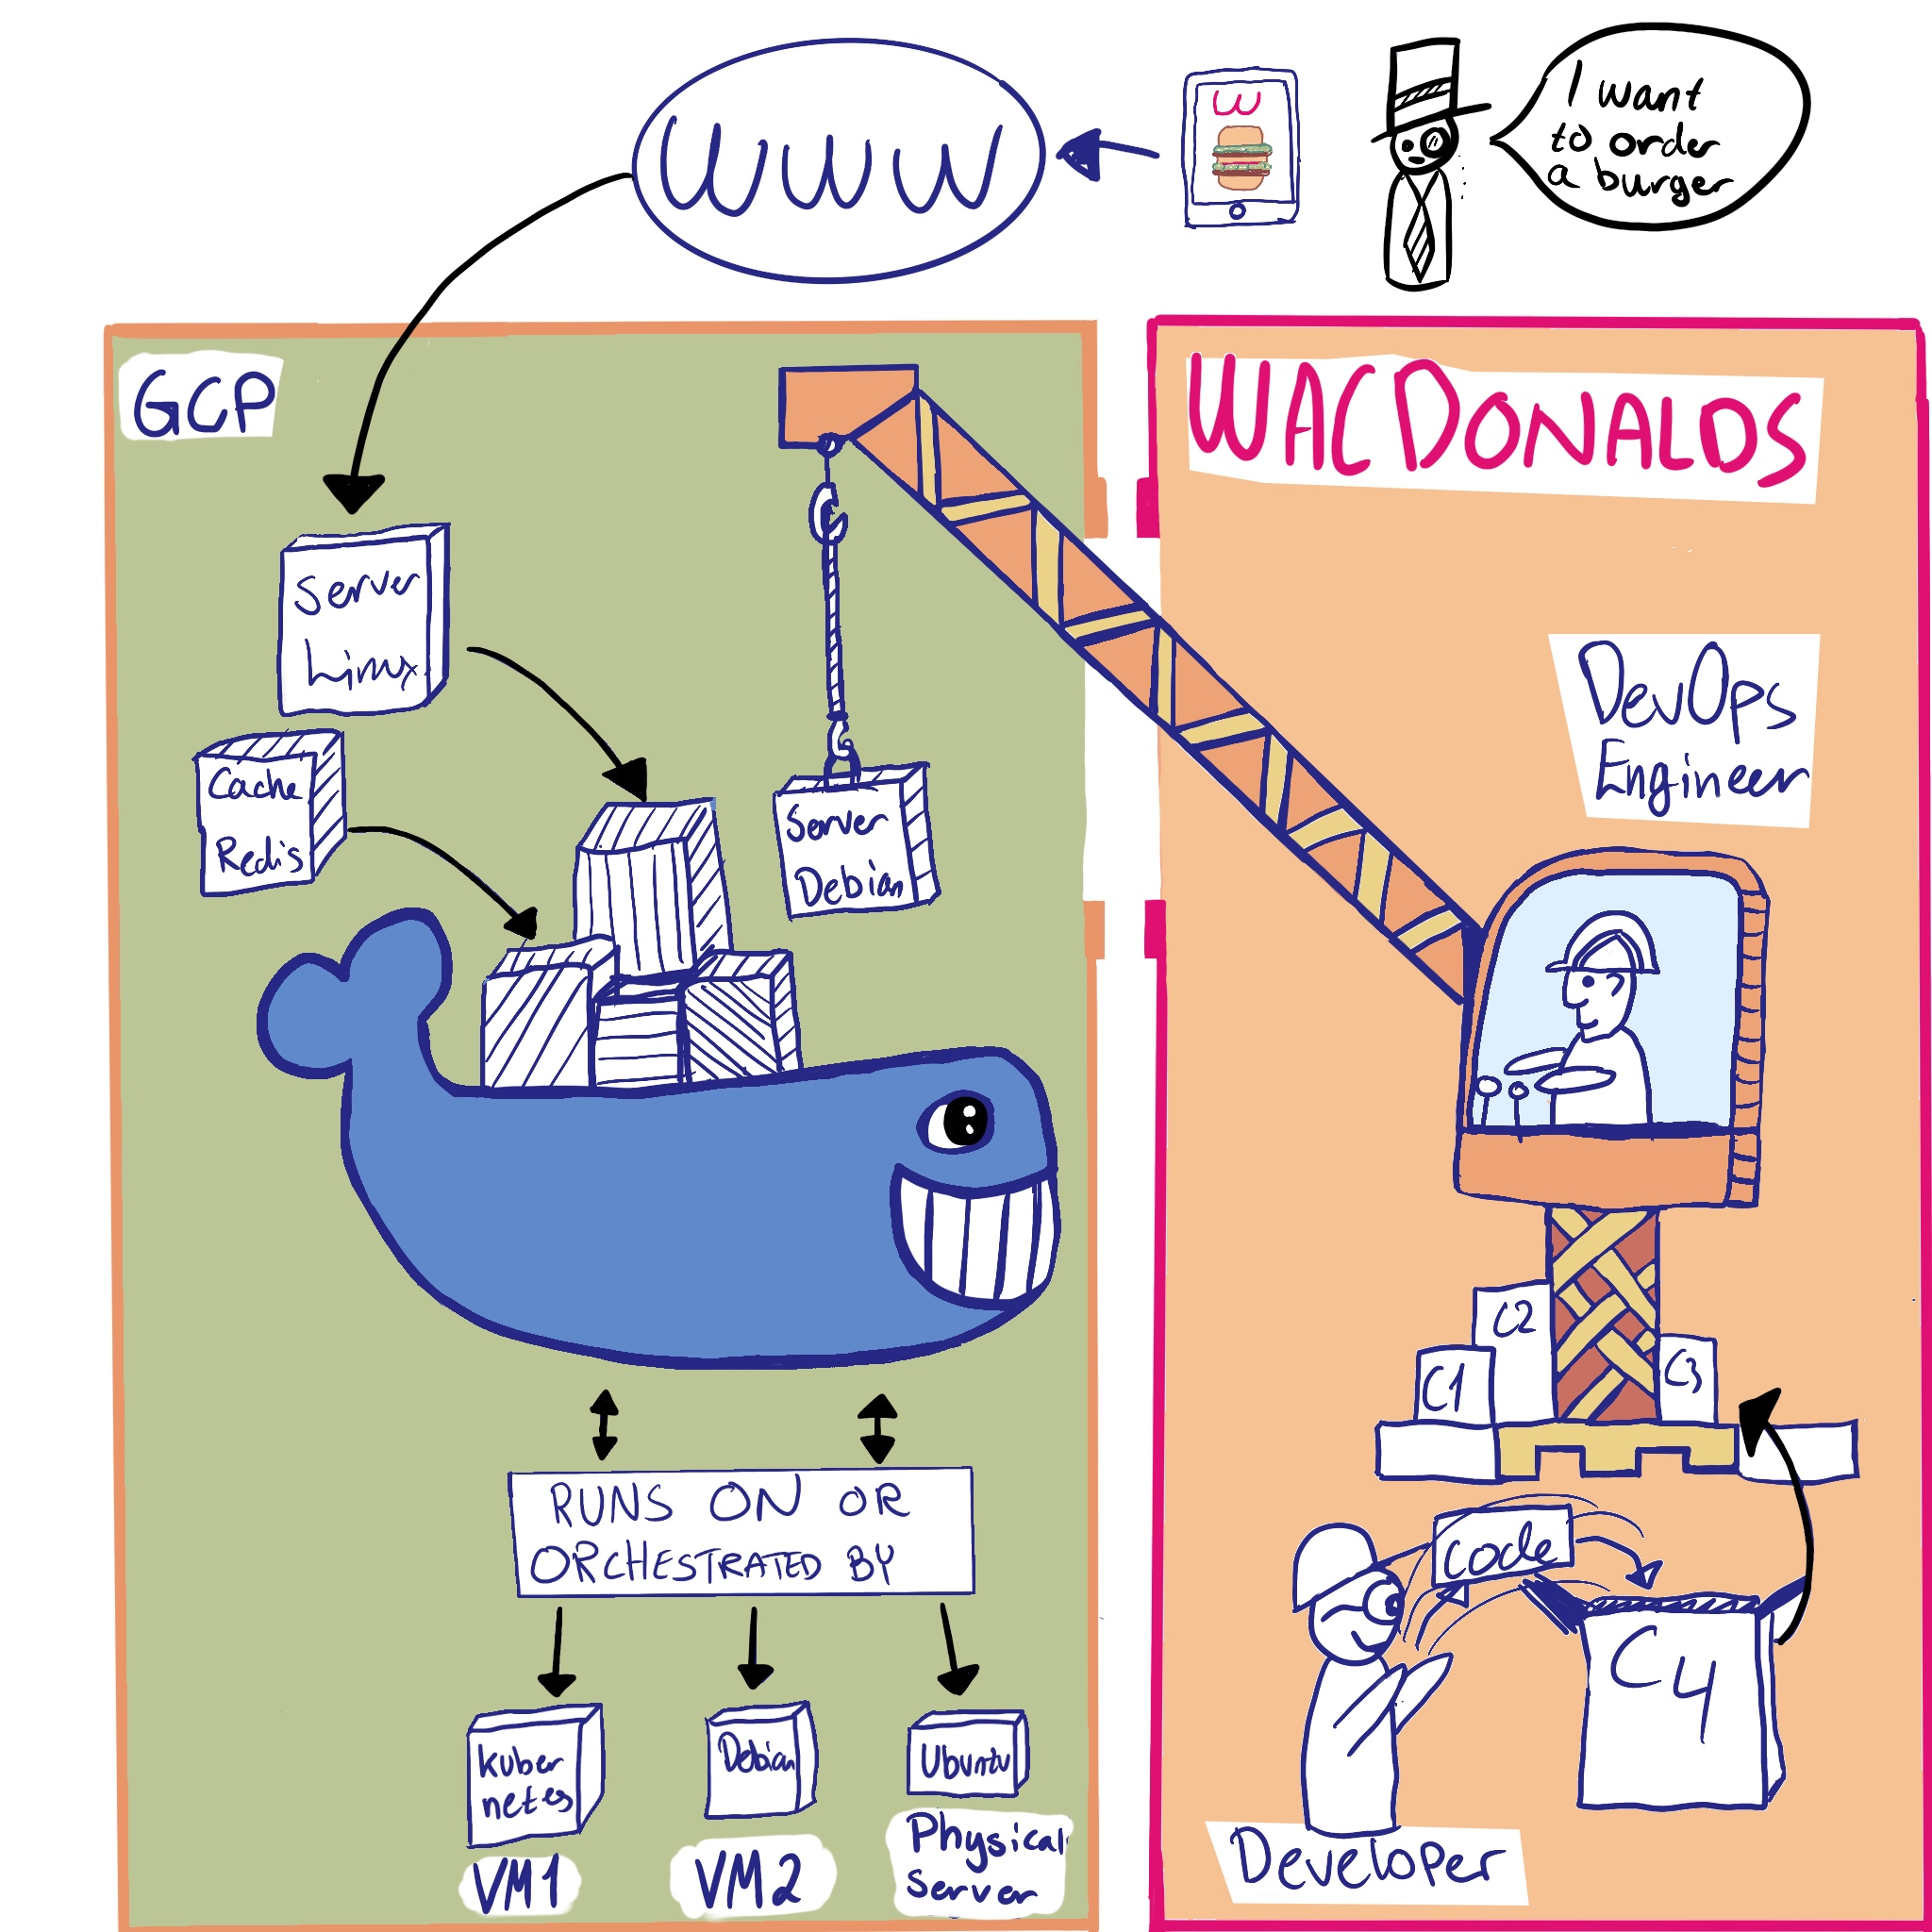
\includegraphics[width=0.8\columnwidth]{assets/docker-wave.jpg}
  \caption{DevOps engineer deploying services as containers on \ac{GCP}.}
  \label{fig:docker}
\end{figure}

Containers are not a perfect solution however, and while they simplify
the means of developing and deploying applications, docker images can
easily reach Gigabytes in image size \citep{durieux2023}, can take a
long time to start up, and building applications that target multiple
platforms can be difficult.

These solutions are more efficient than manually installing an operating
system on a machine, but they still have leave a large footprint. Is
there a more efficient way to package and deploy our programs? \ac{Wasm}
and \ac{WASI}, as mentioned in epigraph of \cref{chap:intro}, has
positioned itself as a potential contender for how applications are
built, packaged and deployed to the cloud.

\section{The Third Wave: WebAssembly Modules}
\label{sect:third-wave}

WebAssembly has had a surge of popularity the past three to four years
when developers discovered that what it was designed for - to truly run
safely inside the browser - translated well into a cloud native
environment as well. Containers have, with the benefits mentioned in
\cref{sect:second-wave}, had a positive impact on the cloud native
landscape. However, with the limitations - like large image sizes, slow
startups and complexity of cross-platform - there is space for exploring
alternative technologies for building our cloud-native applications.

WebAssembly is a compilation target with many languages adopting
support, and by itself, it is sandboxed to run in a WebAssembly \ac{VM}
without access to the outside world, meaning that it cannot access the
underlying system. This means that a ``vanilla'' WebAssembly module
cannot write to the file system, update a Redis cache or transmit a POST
request to another service.

To make this possible, the WebAssembly System Interface project was
created. This project allows developers to write code that compiles to
WebAssembly that can access the underlying system. This is the key
project that turned many developers onto the path of exploring
WebAssembly as a potential contender for building cloud applications.
With WebAssembly, developers can write programs in a programming
language that supports it as a compilation target, such as Rust, C, C++,
Go, and build tiny modules that can run on a WebAssembly runtime. These
WebAssembly runtimes can run on pretty much any architecture with ease,
the resulting binary size are quite small, and the performance is
near-native. These perks combined with the potential for reduced
overhead, smaller image sizes, and faster startup times make WebAssembly
and \ac{WASI} a promising candidate for the third wave of cloud compute
with a lower impact on the environment.

\begin{figure}[H]
\centering
  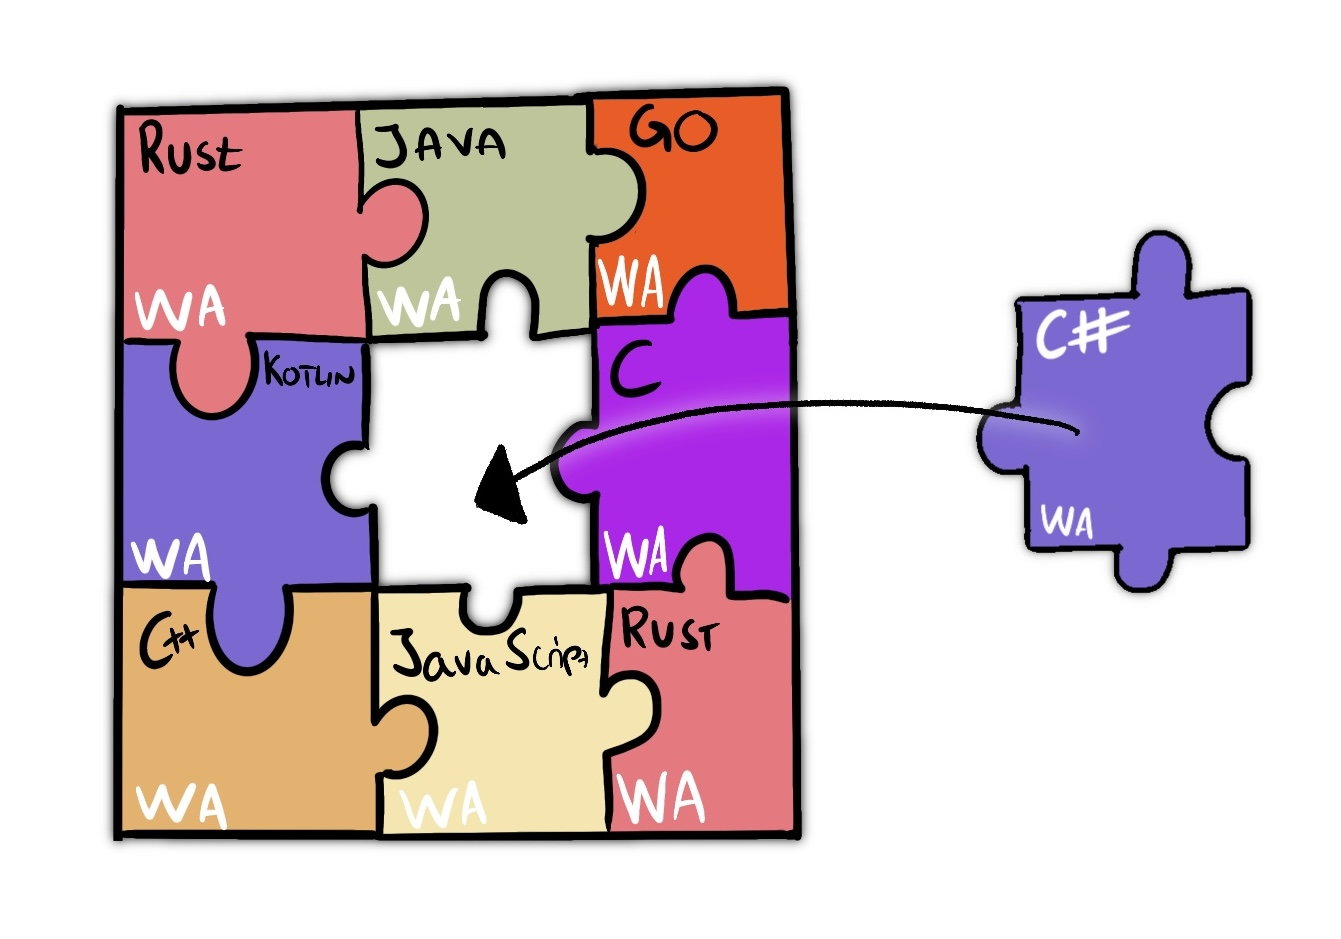
\includegraphics[width=0.8\columnwidth]{assets/wasm-wave.jpg}
  \caption{An example polyglot app built with different languages that all
compile to \ac{Wasm} and can interface together.}
  \label{fig:wasm-wave}
\end{figure}

In summary, the three waves of cloud computing - virtual machines,
containers, and now \ac{Wasm} with \ac{WASI} - represent the industry's
pursuit of more efficient, scalable and reliable solutions for building
cloud applications. While each wave has attempted to tackle pressing
challenges of its time, it is exciting to see how \ac{Wasm} and
\ac{WASI} can be leveraged in this third wave and see if it is promise
of more efficient applications can lead to reducing the environmental
impact of ICT.

\newpage

\chapter{Background}
\label{chap:background}

\setlength\epigraphwidth{.8\textwidth}

\epigraph{\itshape  
We were interested in
applications that needed to start, run to completion, and shut down nearly
instantly. Examples of this are AWS Lambda and Azure Functions. But those were
built on VMs, which are slow to start. So they had to pre-warm huge numbers of
VMs, which sat idle until they received a request. We were looking for a more
efficient runtime that could cold-start in under one millisecond. And that’s
what brought us to WebAssembly.
}{---Matt Butcher, \textit{CEO of Fermyon}}

\section{Cloud Computing Overview}
\label{sect:cloud-overview}

Cloud computing, commonly referred to as ``\emph{the cloud}'', refers to
the delivery of computing resources served over the internet, as opposed
to traditional on-premise hardware setups. The \ac{NIST} defines cloud
computing like so:

\begin{tcolorbox}[
  definitionstyle,
  title=NIST definition of Cloud Computing,
]
Cloud computing is a model for enabling ubiquitous, convenient, on-demand
network access to a shared pool of configurable computing resources (e.g.,
networks, servers, storage, applications, and services) that can be rapidly
provisioned and released with minimal management effort or service provider
interaction. \\

\hfill \citep{nist-def}

\end{tcolorbox}

Cloud computing traces its root back to the 1960s, with the Compatible
Time-Sharing System (CTSS) project at MIT, which demonstrated the
potential for multiple users accessing and sharing computing resources
simultaneously \citep{crisman1963}. While CTSS was a localized system,
it paved the way for the concept of shared computing resources, a
fundamental principle of cloud computing.

Over the following decades, advancements in networking, virtualization
and the ubiquity of the internet led to the development of todays
sophisticated cloud services. The term ``cloud computing'' was first
coined in the year 1996 by Compaq,
\citep{favaloroInternetSolutionsDivision1996}, but it was not until
Amazon launched its subsidiary \ac{AWS} in the 2006 that the adoption
became wide spread.

The launch of \ac{AWS} Amazon S3 cloud service in March 2006, followed
by Elastic Compute Cloud (EC2) in August the same year
\citep{barrAmazonEC2Beta2006}, marked a major turning point in
application development and deployment, and popularized cloud computing.
EC2, as an Infrastructure-as-a-Service platform, empowered developers to
run virtual machines remotely. By providing these services over the
internet on a pay-as-you-go basis, \ac{AWS} drastically lowered the bar
for accessing computing resources, making it easier and more
cost-effective for businesses and developers to build and deploy
applications without the need for considerable upfront investment in
hardware and infrastructure.

With the success of \ac{AWS}, other major technology companies saw their
fit to enter the cloud computing market. In 2008, Google launched the
Google App Engine \citep{mcdonaldIntroducingGoogleApp2008}, a platform
for building and hosting web applications in Google's data centers.
Microsoft followed with the launch of Azure in 2010, its cloud computing
platform that offers a range of services comparable to \ac{AWS}.

The rapid growth of cloud computing also fueled the rise of DevOps
practices and containerization technologies like Docker, which
facilitate the development, deployment and management of applications on
the cloud. Orchestration tools like Docker Swarm and Kubernetes further
simplify the process of managing and scaling containerized applications
across cloud enviroments \citep{bernsteinContainersCloudLXC2014}.

Today, cloud computing has become an essential part of modern IT
infrastructure, where major cloud provides, like \ac{AWS}, Microsoft and
Google, continue to innovate and expand their offerings. Cloud computing
has also enable new paradigms like serverless computing and edge
computing, allowing for even more efficient and distributed computing
models. \citep{baldiniServerlessComputingCurrent2017}

\section{Energy Consumption and Sustainability in Cloud Computing}

A major drawback of cloud computing is the increasing energy consumption
required to power data centers. With the increased demand for energy
consumption, comes an increased impact on the environment. As mentioned
in \cref{chap:intro}, the ICT industry accounts for an estimated 2.1\%
to 3.9\% of global greenhouse emissions \citep{freitag2021}. According
to the International Energy Agency (IEA), data centers across the globe
consumed between from 240 to 340 TWh, accounting for 1 to 1.3\% of the
global electricity use.

In Norway, for example, Google is constructing a data center in Skien,
expected to be fully operational by 2026. As of April 2024, they have
been granted a capacity of 240 Megawatts, but they have applied for a
total capacity of 860 Megawatts
\citep{rivrudInvesteringenAvGooglesenter2024}. At full capacity at 860
MW, Google's data center is aiming to consume 7.5 TWh each year, and
according to Google's most recent sustainability report, they consumed a
total of 22.29 TWh globally in 2022 \citep{Google2023Environmental2023}.
In other words, in 2026 the data center in Skien alone is projected to
consume \textasciitilde33\% of the energy Google consumed globally in
2022. The energy consumption in Norway is projected to reach 150-158 TWh
in 2026 \citep{gunnerodStatnettAnalyse2022}, meaning that the data
center in Skien could account for 5\% of the energy consumption in the
country. \Cref{fig:skienvsnorway} below illustrates the amount of energy
the new data center will consume compared to Norway.

\vspace{0.25cm}

\begin{figure}[H]

{\centering 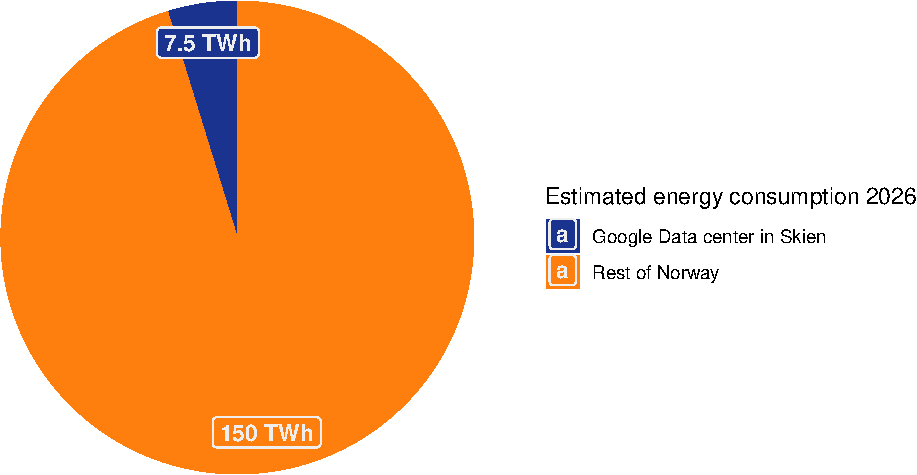
\includegraphics[width=0.8\linewidth]{thesis_files/figure-latex/skienvsnorway-1} 

}

\caption{Projected energy consumption in 2026: Skien data center and Norway.}\label{fig:skienvsnorway}
\end{figure}

\todo[inline=true]{Consider this feedback from Michael: Google also does not
make it rain more. If Google come and buys all the green energy in the area, it
will just mean that others will use more black energy. They don not build new
infrastructure. And this is only for Googles "usage". Not the users and network
infrastructure.}

The flipside of this, is that Google is commited to reach a net-zero
carbon footprint by 2030, and the data center in Skien is built to
reflect this. Google has been carbon neutral since 2007 and has matched
100\% of its annual electricity consumption with renewable energy since
2017 \citep{googleTrackingOurCarbonFree}. Norway's abundant hydropower,
rising wind power production, investment into solar energy and other
renewable energy sources make it an ideal location for building data
centers aiming to be powered by renewable energy
\citep{norwegian-energyElectricityProduction2023}.

Like Google, other major cloud providers have set ambitious targets for
renewable energy adoption and have invested in large-scale renewable
projects. Microsoft has committed to shifting to 100\% renewable energy
by 2025 for all its data centers, buildings and campuses, and to be
carbon \emph{negative} by 2030 \citep{smithMicrosoftWillBe2020}, while
Amazon has pledged to transition to 100\% renewable energy by 2030 for
its cloud subsidiary and to have a net-zero carbon footprint by 2040
\citep{amazonClimatePledge2019}. These efforts have contributed to
reducing greenhouse gas emissions in the cloud computing industry, but
this commitment is not universally adopted, and many data centers still
rely on electricity generated by fossil fuels, a leading contributor to
climate change \citep{mytton2020}.

\todo{Feedback fra ingvild: include that data centers also increase the demand
for power, so more power demand => more nature gets torn down to accomadate for
the increase in demand.}

Several factors make up the energy consumption required to service a
data center. One of these factors is cooling down the servers while
running, and a study from 2017 discovered that cooling accounted for
about 38\% of total energy consumption in data centers, ranging from
21\% to 61\% depending the effectiveness of the facility's heating,
ventilation, and air conditioning (HVAC) system
\citep{niReviewAirConditioning2017}.

One innovative example of attempting to mitigate the environmental
impact of cooling data centers can be found by data center providers
like DeepGreen\footnote{\url{https://deepgreen.energy/faqs/}}, who
submerge their servers into dielectric fluid, which gets warmed up by
the excess heat of the computers. This heat is then transferred to a
host's hot water system via a heat exchange and used for heating up
swimming pools in London. Another broad strategy cloud providers opt for
is the implementation of power management techniques, such as dynamic
voltage and frequency scaling (DVFS), which adjusts the power
consumption of servers based on workload demands
\citep{beloglazovEnergyawareResourceAllocation2012}.

Virtualization and resource pooling, two key components of cloud
computing, also contribute to energy efficiency. By consolidating
virtual machines onto shared physical servers, cloud providers are able
to improve resource utilization and reduce the energy consumption of
their data centers. \citep{beloglazovEnergyawareResourceAllocation2012}

\section{Virtualization and Virtual Machines}
\label{sect:virtual}

Virtualization is the process of creating a virtual version of a
physical resource such as an operating system, a server, a storage
device, or a network resource
\citep{chiuehSurveyVirtualizationTechnologies2005}. Virtualization allow
multiple virtual instances to share the underlying physical hardware,
enabling more efficient resource utilization and consolidation.

One of the most common forms of virtualization is the creation of
\ac{VMs}. \citet{barhamXenArtVirtualization2003} described that a
virtual machine is a software-based emulation of a physical computer
system, including its processor, memory, storage, and network
interfaces. Furthermore they describe that \ac{VMs} run on top of a
hypervisor, a software layer that manages and allocates the physical
hardware resources to the virtual machines.

\Cref{vm-figure} below illustrates virtual machines running in such an
environment.

\begin{figure}[H]
\centering
  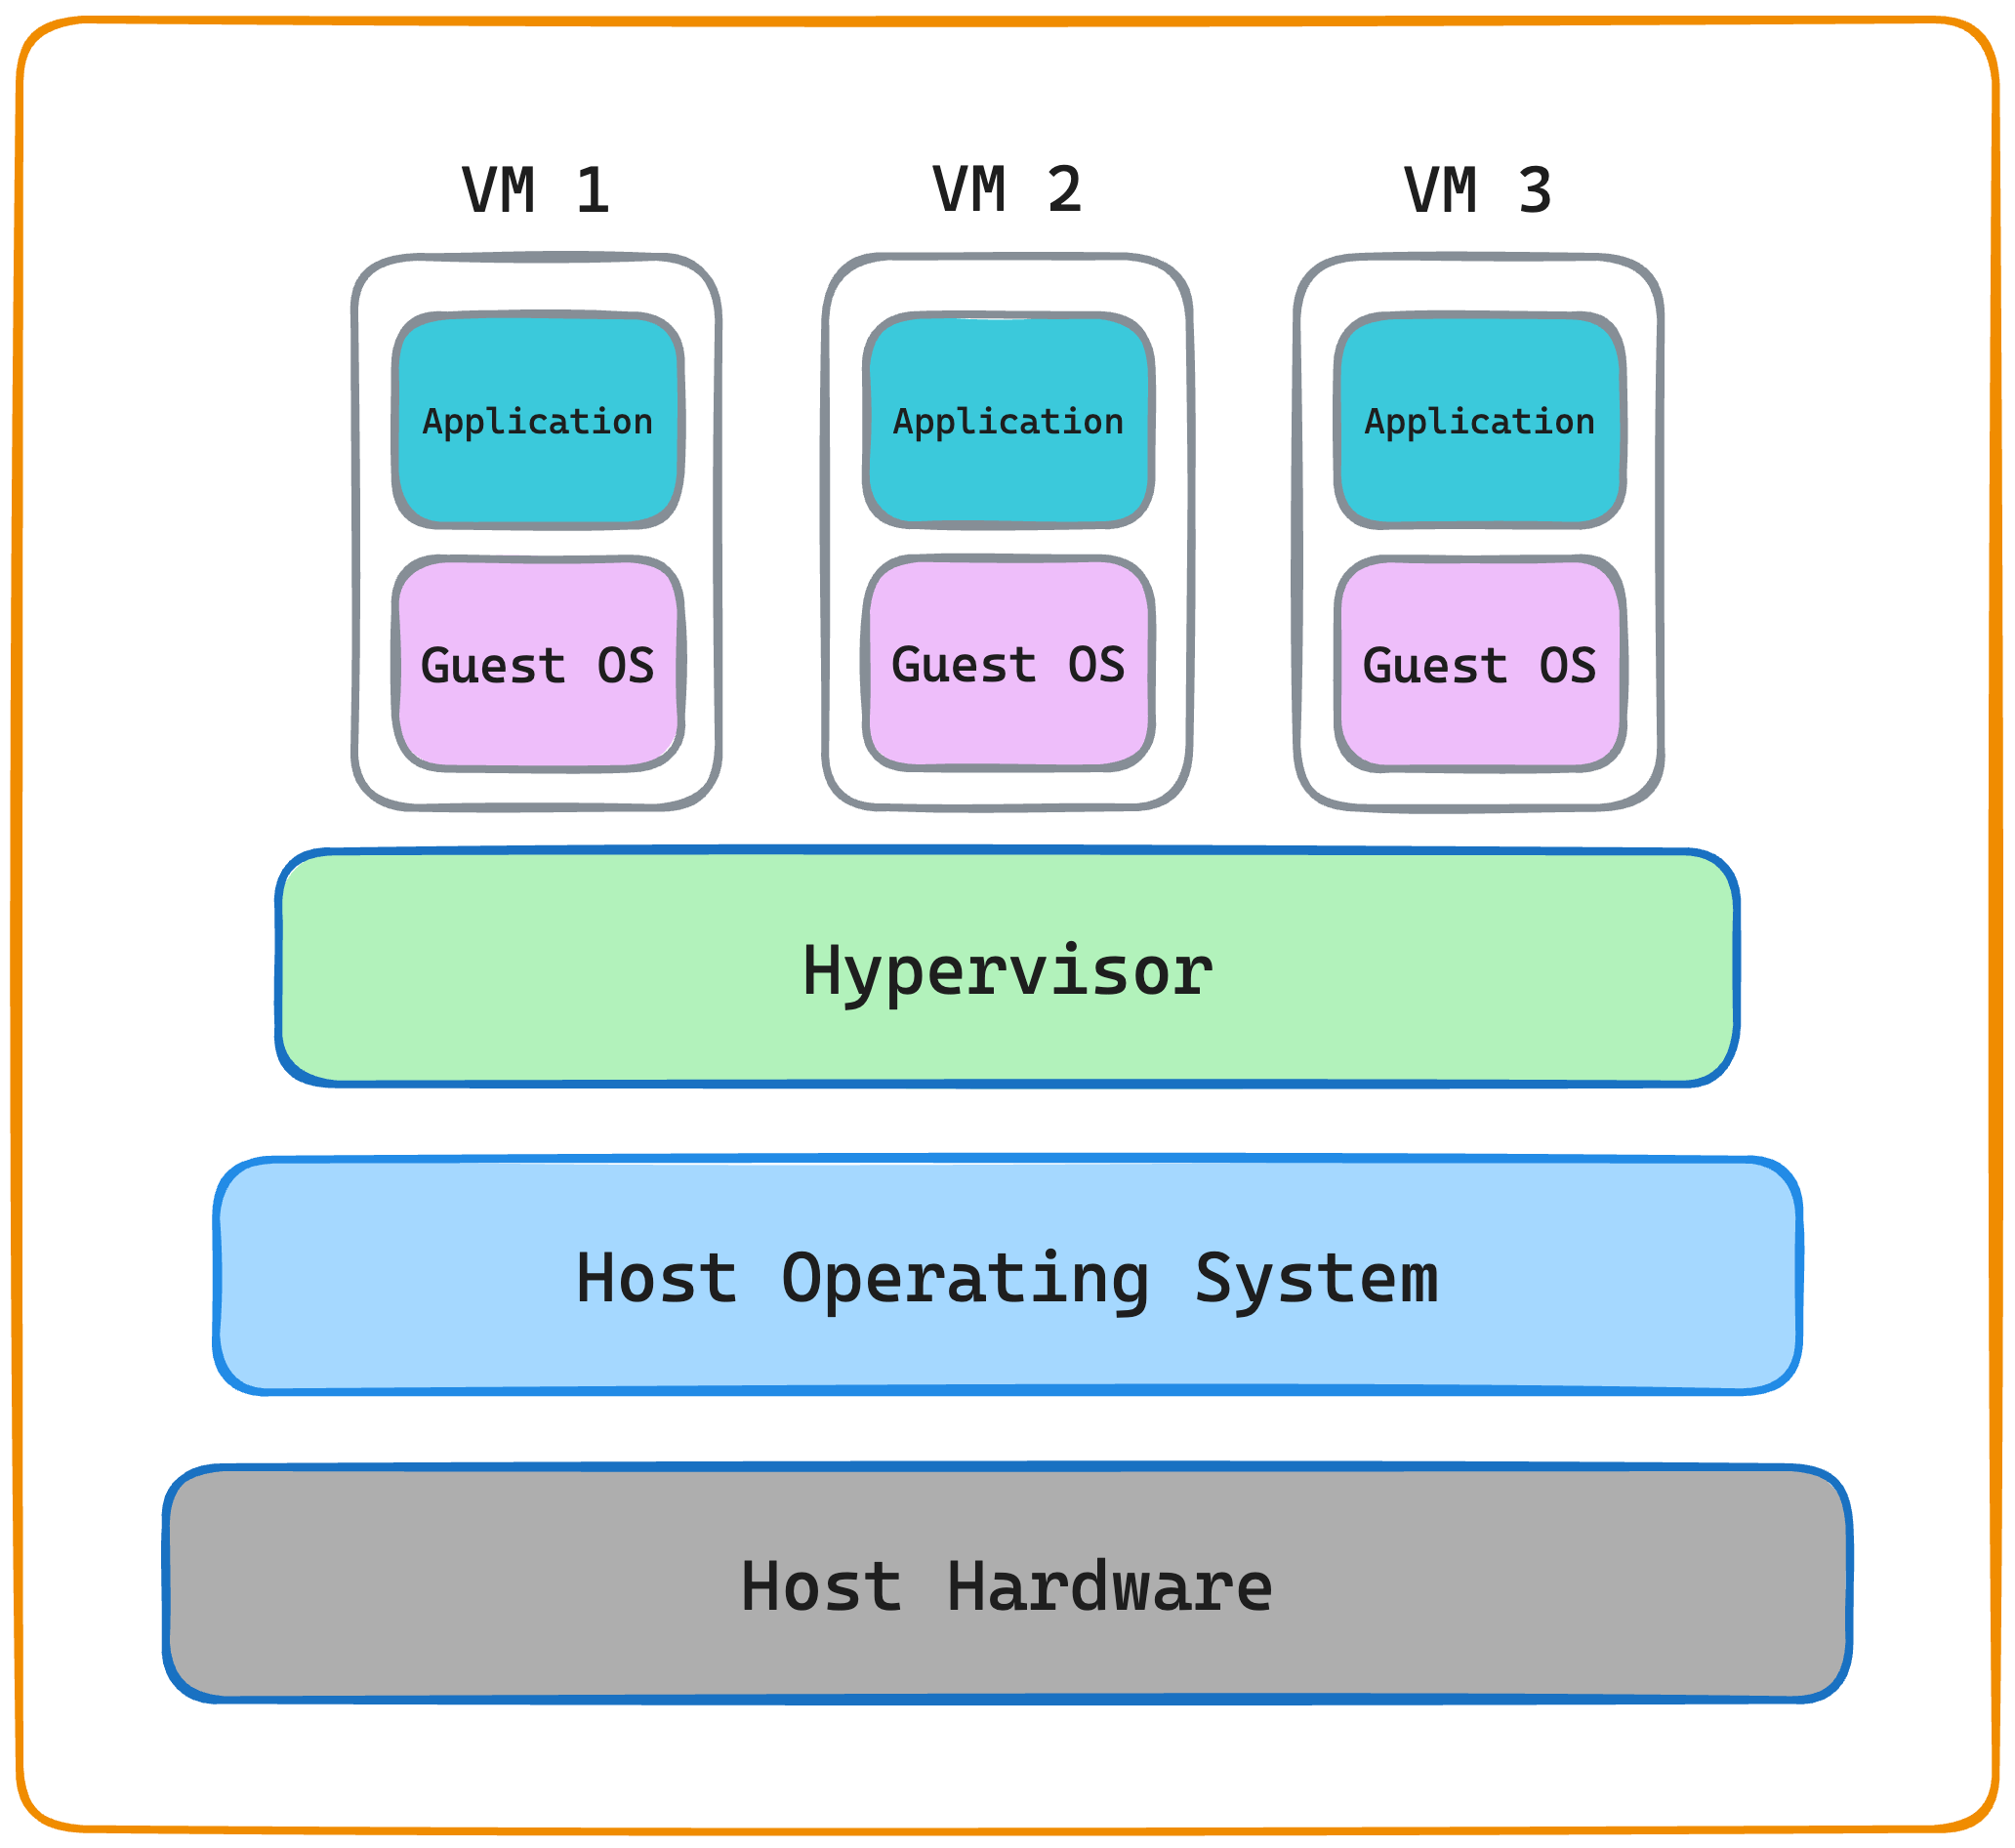
\includegraphics[width=0.7\columnwidth]{assets/3.2-vm-figure.png}
  \caption{Virtual machines running on top of Hypervisor on a computer.}
  \label{vm-figure}
\end{figure}

By running several virtual machines on the same physical server, data
centers can drastically decrease the number of physical machines
physical machines needed to operate, leading to a reduction in energy
consumption \citep{kaplanRevolutionizingDataCenter2008}.

\section{Containers and Container Orchestration}
\label{sect:containers}

While virtual machines provide isolation at the hardware level,
containers offer a more lightweight form of virtualization by isolating
applications at the operating system level
\citep{merkelDockerLightweightLinux2014}. Containers share the host
operating system's kernel, enabling them to be more lightweight and
efficient compared to traditional virtual machines. They can run
physical servers, as well as on \ac{VMs}
\citep{bernsteinContainersCloudLXC2014}.

\citet{merkelDockerLightweightLinux2014} also explains that containers
package an application and its dependencies into a single unit. This
includes libraries, configuration files and other necessary files. This
allows applications to be deployed consistently across different
environments, ensuring predictable behavior and reducing compatibility
issues \citep{sergeevDockerContainerPerformance2022}

By enabling more granular and efficient use of system resources,
containers contribute to lower energy usage compared to virtual machines
due to their lightweight nature and faster startup times
\citep{shirinbabPerformanceEvaluationContainers2020}. The adoption of
containerization technologies have been shown to optimize energy costs,
as containers allow for a higher density of applications running on the
same physical hardware without the overhead associated with full
virtualization
\citep{cuadrado-corderoComparativeExperimentalAnalysis2018}.

Docker is one of the most widely adopted container platforms, providing
tools for building, shipping, and running applications in containers
\citep{merkelDockerLightweightLinux2014}. Docker containers are based on
open standards and can run on various operating systems and cloud
platforms \citep{sergeevDockerContainerPerformance2022}.
\Cref{container-figure} below illustrates how containers run ontop of a
Docker Engine on a virtual or physical machine.

\begin{figure}[H]
\centering
  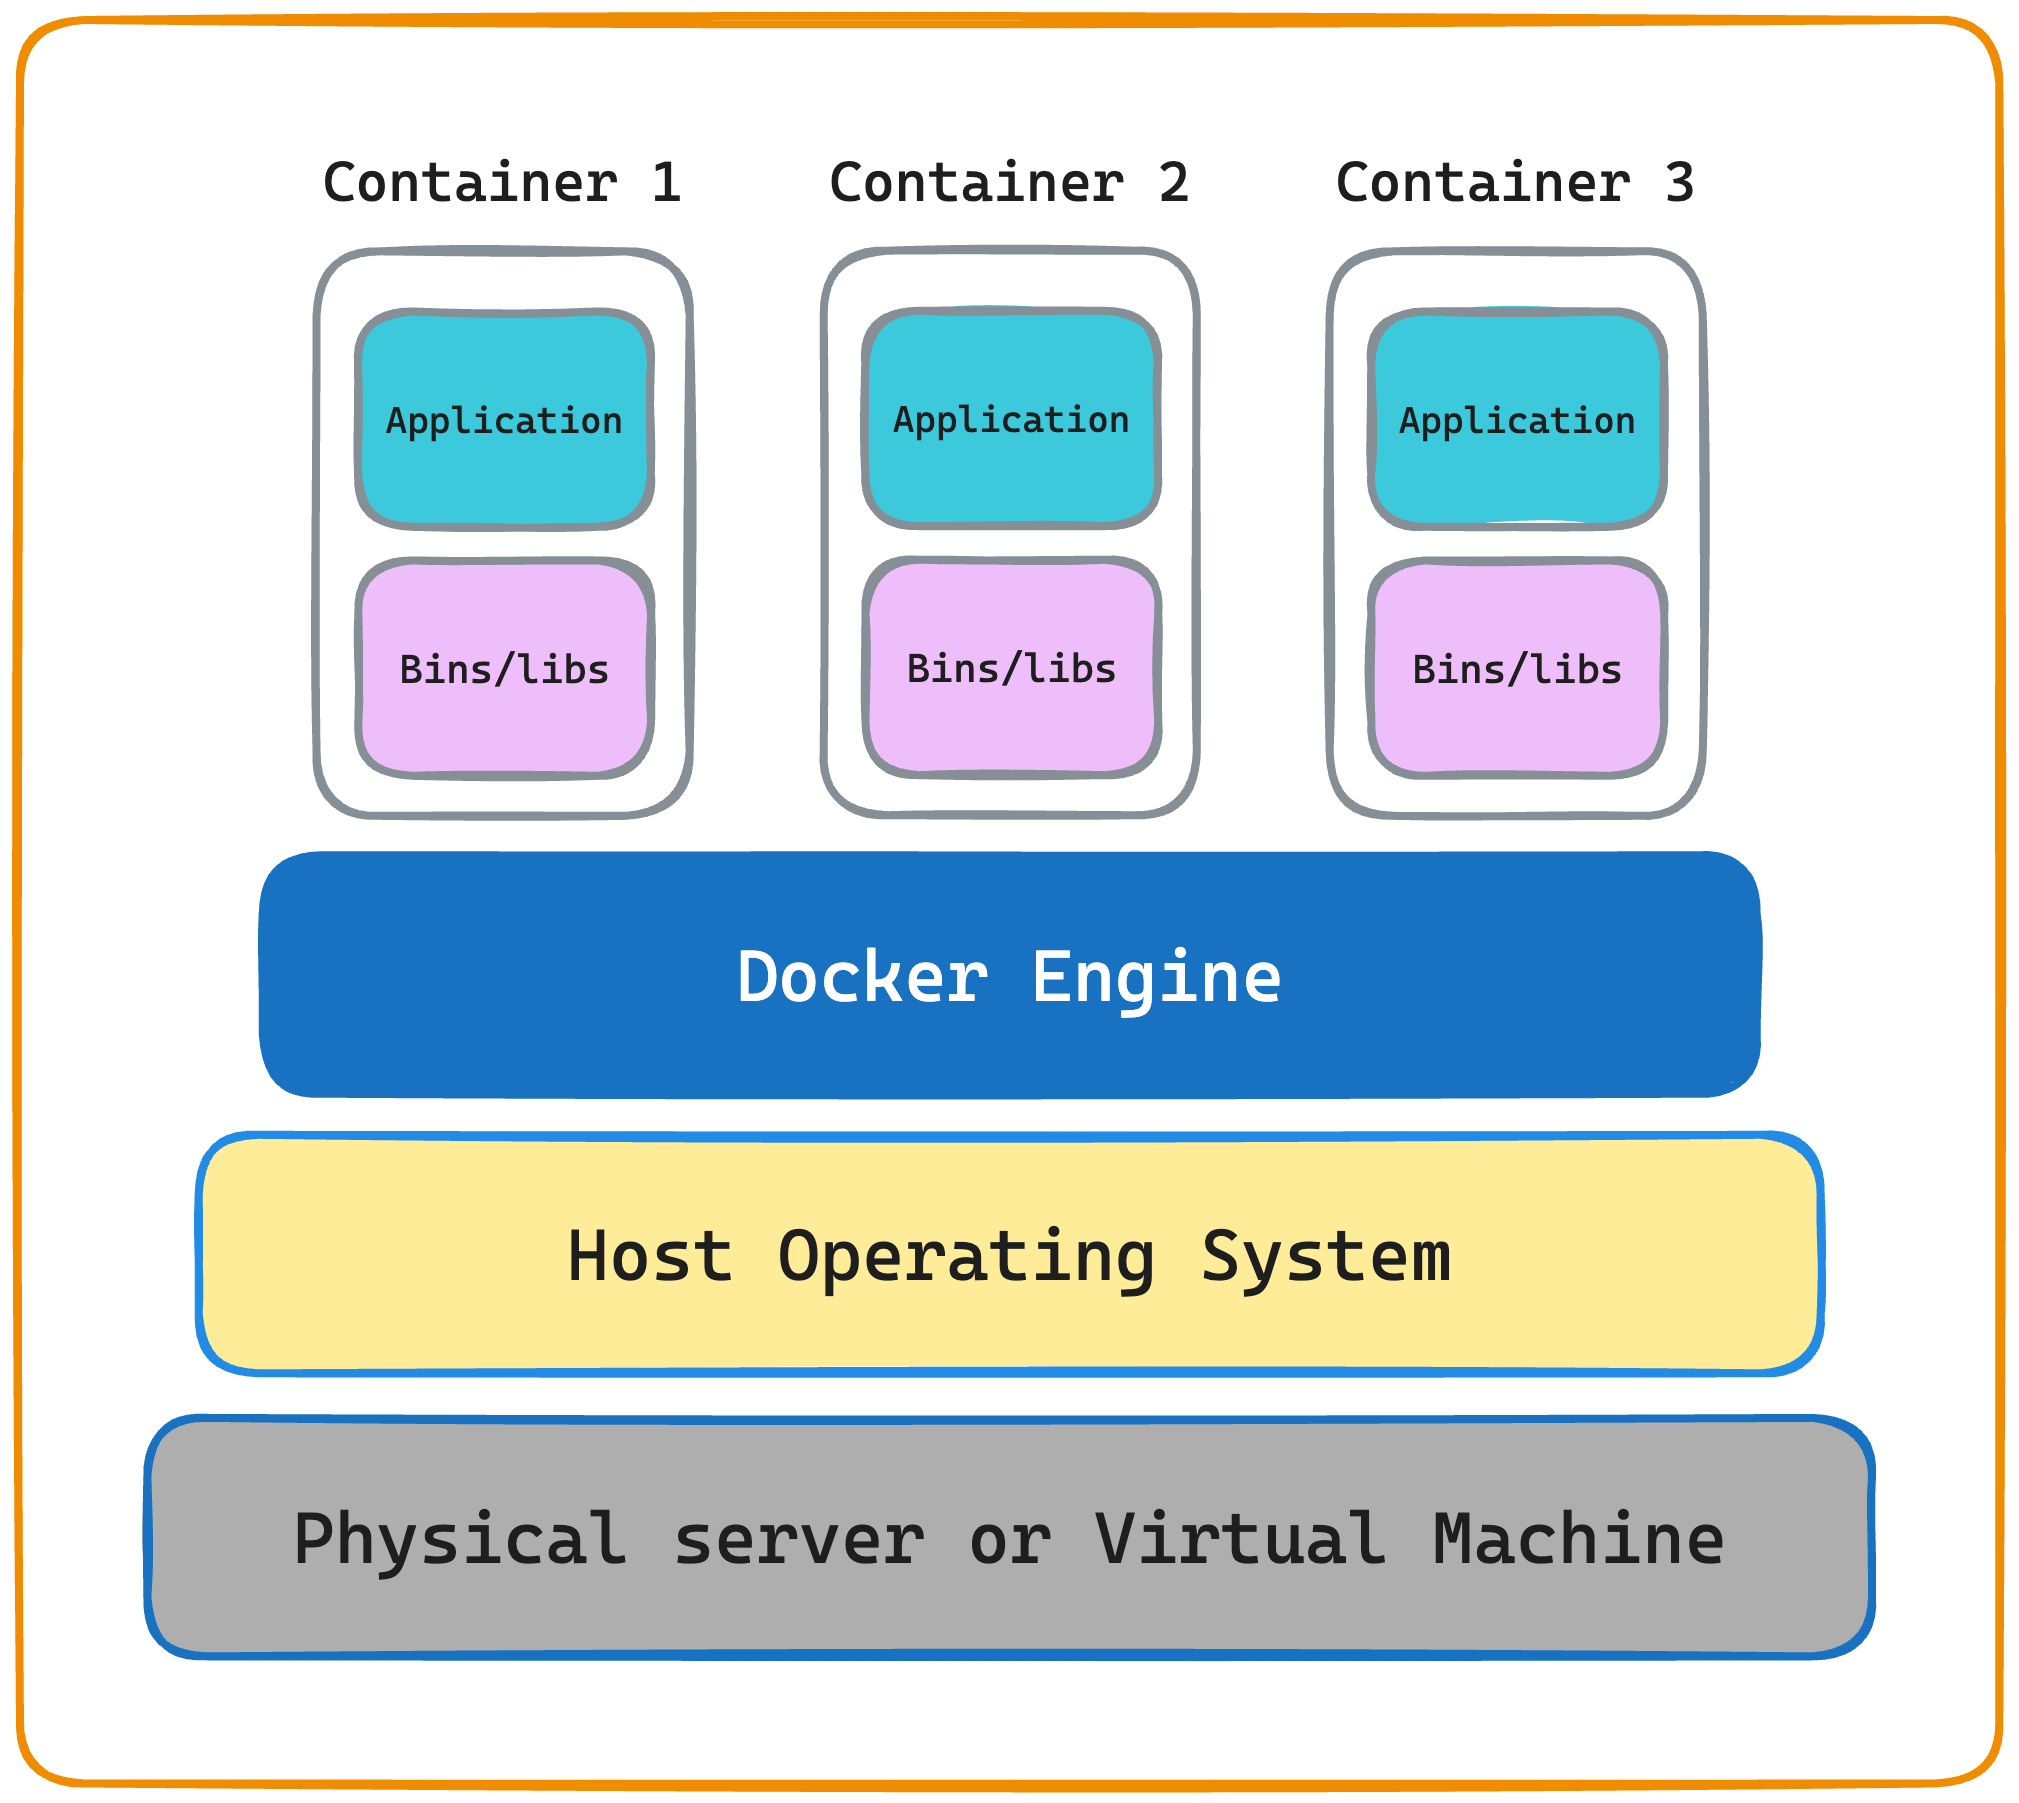
\includegraphics[width=0.7\columnwidth]{assets/3.3-container-figure.png}
  \caption{Containers running on the Docker Engine}
  \label{container-figure}
\end{figure}

As the number of containers in an environment grows, managing and
orchestrating them becomes increasingly complex. Container orchestration
tools, such as Kubernetes and Docker Swarm, help automate the
deployment, scaling, and management of containerized applications across
multiple hosts \citep{burnsBorgOmegaKubernetes2016}.

These tools provide features like:

\begin{enumerate}
\def\labelenumi{\arabic{enumi}.}
\tightlist
\item
  Automated deployment and scaling: Containers can be automatically
  provisioned, scaled up or down based on demand, and load-balanced
  across multiple hosts \citep{burnsBorgOmegaKubernetes2016}.
\item
  Self-healing and monitoring: Orchestration tools can monitor the
  health of containers and automatically restart or reschedule them in
  case of failures \citep{kubernetesKubernetes}.
\item
  Service discovery and load balancing: Applications running in
  containers can be easily discovered and accessed by other services,
  enabling microservice architectures \citep{kubernetesKubernetes}.
\end{enumerate}

Container orchestration has become an essential component of modern
cloud-native architectures, enabling efficient management and scaling of
containerized applications in dynamic environments.

\section{Serverless Computing}

Serverless computing has emerged as an alternative to traditional
infrastructure management approahces, such as managing physical servers
or building developer platforms as described in \Cref{sect:containers}
\citep{baldiniServerlessComputingCurrent2017}. In serverless computing,
the underlying infrastrucutre is abstracted away, allowing developers to
focus on writing code and deploying programs without the need to
provision or manage servers
\citep{baldiniServerlessComputingCurrent2017,robertsServerlessArchitectures2018}.
\citet{castroRiseServerlessComputing2019} defines serverless as such:

\begin{tcolorbox}[
  definitionstyle,
  title=Serverless definition,
]
Serverless computing is a platform that hides server usage from
developers and runs code on-demand automatically scale and billed only for the
code running. \\

\hfill \citep{castroRiseServerlessComputing2019}

\end{tcolorbox}

According to \citet{baldiniServerlessComputingCurrent2017}, in a
serverless model, the cloud provider is responsible for managing the
infrastructure, including resource allocation, scaling, and maintenance.
This approach enables more efficient resource utilization, as resources
are dynamically allocated based on demand. Furthermore, developers can
deploy containers or functions independently, promoting modularity and
scalability.

On top of this, severless computing offers several more benefits,
including:

\begin{enumerate}
\def\labelenumi{\arabic{enumi}.}
\tightlist
\item
  Reduced operational overhead: Developers do not need to manage servers
  or infrastructure, freeing up time and resources for application
  development \citep{baldiniServerlessComputingCurrent2017}.
\item
  Faster time-to-market: With serverless, developers can quickly deploy
  and iterate on functions without the need for time consuming
  infrastructure setup \citep{adzicServerlessComputingEconomic2017}.
\item
  Cost efficiency: Serverless platforms typically employ a pay-per-use
  pricing model, where users are charged based on the actual execution
  time and resources consumed by their applications
  \citep{eismannReviewServerlessUse2021}.
\end{enumerate}

However, serverless architectures also introduce certain challenges,
such as:

\begin{enumerate}
\def\labelenumi{\arabic{enumi}.}
\tightlist
\item
  Potential vendor lock-in: Serverless platforms may have
  provider-specific APIs and services, which can make it challenging to
  change providers or migrate applications
  \citep{gottliebServerlessDataLockin2018}.
\item
  Cold start latencies: Containers or functions that have not beeen
  invoked recently may experience longer startup times, cold starts,
  which can impact application performance
  \citep{golecColdStartLatency2023}.
\item
  Resource overhead and efficiency: Serverless platforms typically rely
  on containerization technologies, such as Docker, to encapsulate and
  isolate function executions. The use of containers can introduce
  resource overhead and impact the efficiency of serverless applications
  \citep{akkusSANDHighPerformanceServerless2018}.
\end{enumerate}

Examples of widely used platforms that build on the serverless model can
be found at the major cloud providers, like Google Cloud Run\footnote{\url{https://cloud.google.com/run}},
\ac{AWS} Fargate\footnote{\url{https://aws.amazon.com/fargate/}} and
Microsoft's \ac{ACI}\footnote{\url{https://azure.microsoft.com/en-us/products/container-instances}}.
These three example platforms allow developers to deploy containers onto
the cloud without worrying about orchestration behind the scenes.

\subsection{Functions-as-a-Service}

\ac{FaaS} is a cloud computing model, derived from serverless, that
allows developers to execute individual functions in response to events
or triggers without needing to manage the underlying infrastructure
\citep{sewakWinningEraServerless2018}.

Examples of these \ac{FaaS} platforms among the big three cloud
providers are; \ac{AWS} Lambda\footnote{\url{https://aws.amazon.com/lambda/}},
Google Cloud Functions\footnote{\url{https://cloud.google.com/functions}},
and Microsoft's Azure Functions\footnote{\url{https://azure.microsoft.com/en-us/products/functions}}.
On FaaS platforms like these, developers write and deploy small,
self-contained functions that perform specific tasks. These functions
are typically stateless and can be written in various programming
languages supported by the FaaS provider
\citep{baldiniServerlessComputingCurrent2017}.

When a function is triggered, the FaaS platform automatically allocates
the necessary resources to execute the function, such as CPU, memory,
and network bandwidth. The platform also handles the scaling of the
function based on the incoming requests, ensuring that the function can
handle varying workloads by itself
\citep{mcgrathServerlessComputingDesign2017}.

FaaS platforms often utilize container technology, like Docker, to
provide an isolated environment for each function execution. Containers
offer several benefits, such as fast startup times, efficient resource
utilization, and the ability to package functions with their
dependencies \citep{vaneykServerlessMorePaaS2018}. However, the use of
containers in FaaS also introduce some challenges including, cold start
latency and the overhead associated with container initialization and
management \citep{wangPeekingCurtainsServerless2018}.

Cold start latency refers to the time it takes for a FaaS platform to
provision a new container instance when a function is invoked after a
period of inactivity. This latency can be significant, especially for
applications with strict performance requirements
\citep{wangPeekingCurtainsServerless2018}. The limitations of containers
in FaaS environments have led to the exploration of alternative
approaches, such as using \ac{Wasm} and \{WASI\}. As Solomon Hykes, the
creator of Docker, stated:

\begin{displayquote}
\textit{ ``If WASM+WASI existed in 2008, we wouldn't have needed to create Docker.
That's how important it is. WebAssembly on the server is the future of cloud
computing. A standardized system interface was the missing link. Let's hope WASI
is up to the task.`` \citep{hykesOne2019} }
\end{displayquote}

This statement highlights the potential of \ac{Wasm} and \ac{WASI} to
face the challenges with containers in FaaS and to provide a more
efficient and platform-agnostic approach to serverless computing, a
potential explored and supported by
\citet{kjorveziroskiEvaluatingWebAssemblyOrchestrated2022}.

\section{WebAssembly and WASI}
\label{sect:wasmwasi}

WebAssembly, commonly referred to as Wasm, is a modern binary
instruction format that has risen to prominence as a versatile
technology across a diverse amount of computing environments,
originating in the web browser. This section introduces the project that
WebAssembly evolved from - \emph{asm.js} - and illustrate how
WebAssembly lets developers write programs in a high-level language and
run them across a multitude of platforms.

\subsection{asm.js}
\label{subsect:asm}

Mozilla released the first version of asm.js in 2013, and it was
designed be a subset of JavaScript, allowing web applications written in
other languages than JavaScript, such as C or C++, to run in the
browser. The intention of asm.js was to enable web applications to run
at performance closer to native code than applications written in
standard JavaScript. A simplified flow for how source code written in
C/C++ is compiled to bytecode that can be executed in the browser can be
found in figure \ref{fig:asm-figure} below.

\begin{figure}[H]
\centering
  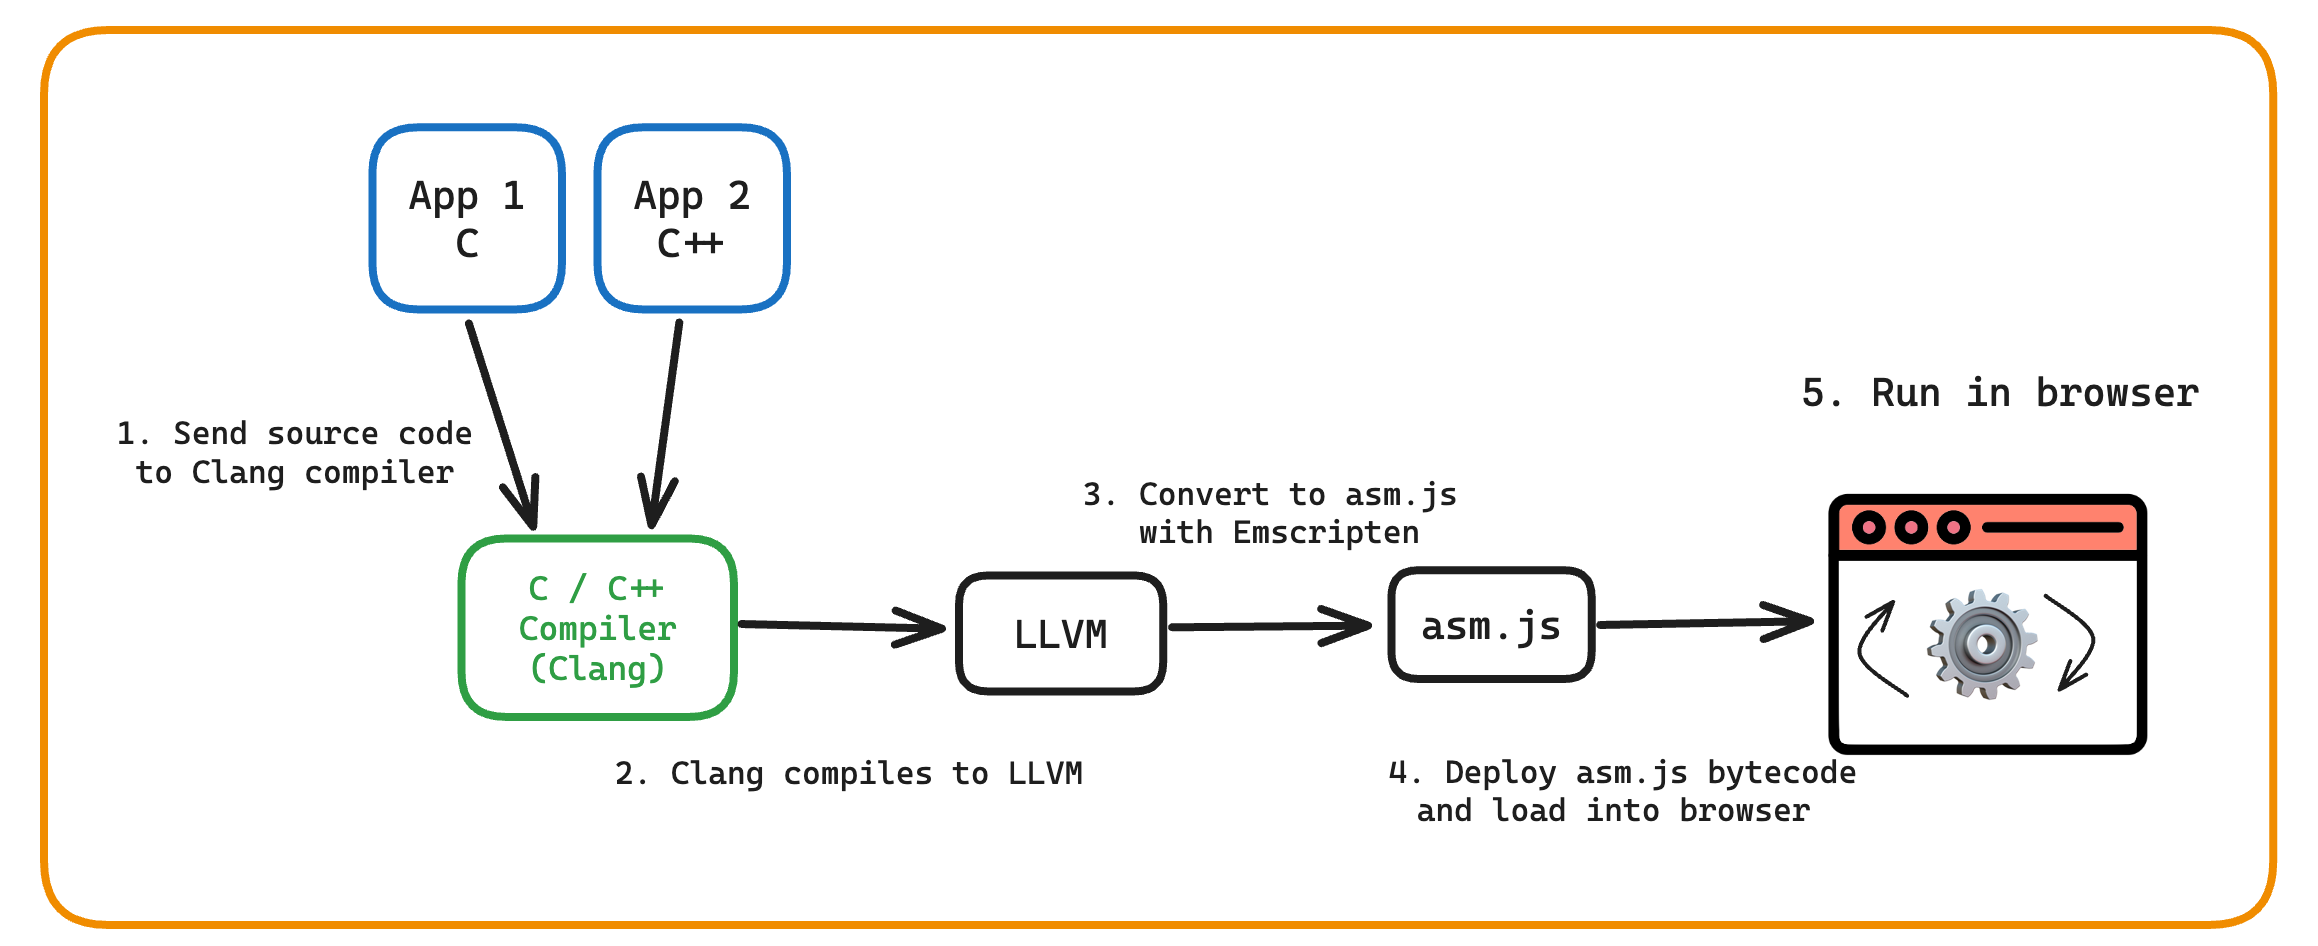
\includegraphics{assets/asm.js-figure.png}
\caption{Source code in C/C++ compiled to asm.js and run in browser}\label{fig:asm-figure}
\end{figure}

While asm.js was a great leap forward, being a subset of JavaScript
limited its scope, leading to its deprecation in 2017 and the
development of a more efficient and portable format
\citep{webassembly.orgFAQWebAssembly}.

\subsection{WebAssembly}

The team at Mozilla built upon the lessons learned from asm.js and went
on to develop WebAssembly, launching the first public version in 2017.
WebAssembly is a low-level code format designed to serve as a
compilation target for high-level programming languages
\citep{haasBringingWebSpeed2017}. It is a binary format that gets
executed by a stack-based virtual machine, comparable to how Java
bytecode runs on the \ac{JVM} \citep{haasBringingWebSpeed2017}. In
\Cref{fig:wasm-browser} below, a simplified flow for compiling web
applications written in different languages can be compiled and run
inside a web browser.

\begin{figure}[H]
\centering
  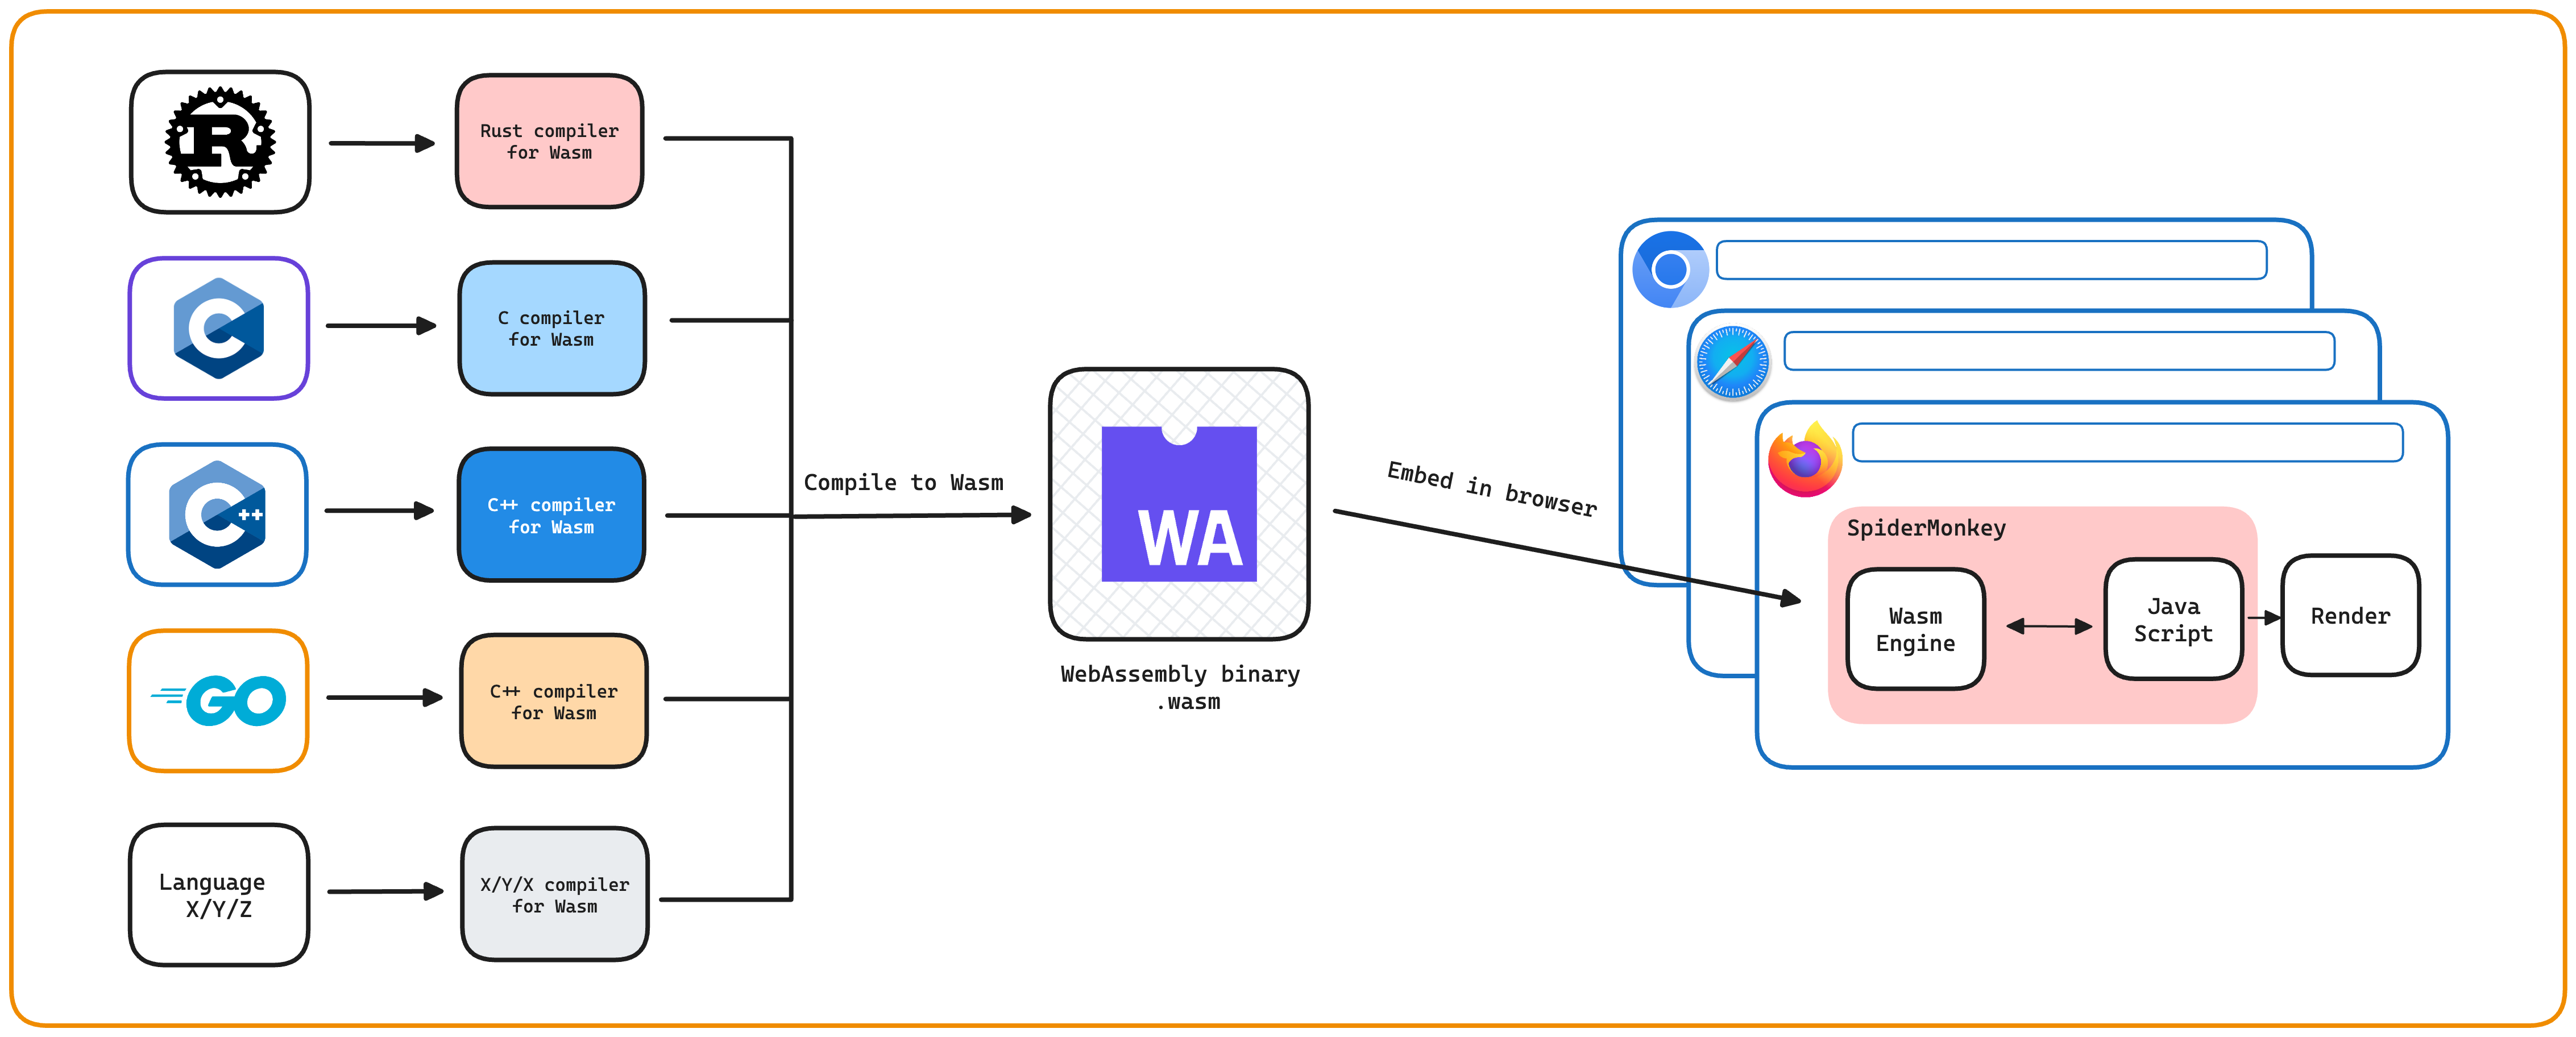
\includegraphics{assets/wasm-browser.png}
  \caption{Source code compiled to WebAssembly and embedded in browser}
  \label{fig:wasm-browser}
\end{figure}

According to \citet{haasBringingWebSpeed2017}, some key features that
the team behind \ac{Wasm} sought out to implement were:

\begin{table}[ht]
\centering
\caption{WebAssembly features}
\begin{tabular}{@{}p{0.3\linewidth}@{\hskip\tabcolsep}p{0.6\linewidth}@{}}
\toprule
\textbf{Feature} & \textbf{Description} \\
\midrule

\rowcolor{green!10} Portability & Wasm can run on different hardware and
operating systems due to its hardware-independent design and sandboxed
execution environment. \\

High Performance & Wasm aims to achieve near-native performance by leveraging
hardware capabilities and ahead-of-time compilation. \\

\rowcolor{green!10} Security & Wasm modules run in a sandboxed environment,
isolated from the host system, with strict memory and control flow limits,
mitigating security vulnerabilities. \\

Modular design & As an open standard with a modular design, Wasm can be
extended and integrated with various programming languages and tools, enabling
broad applications beyond web browsers. \\

\rowcolor{green!10} Efficient compression & Wasm's binary format is designed for
efficient compression, reducing code size and improving download times,
especially on resource-constrained devices. \\

\bottomrule
\end{tabular}
\label{table:wasm_benefits}
\end{table}

By addressing performance, security and portability concerns, \ac{Wasm}
offers an alternative to traditional approaches for running untrusted
code on the web and in other computing environments, such as cloud and
edge computing \citep{haasBringingWebSpeed2017}.

\subsection{WebAssembly System Interface}

While \ac{Wasm} was initially designed to run in web browsers, its
potential for use in other environments, such as cloud and edge
compuitng, led to the development of the WebAssembly System Interface.
\ac{WASI} is a modular system interface that provides a standardized set
of functions for interacting with the host operating system, enabling
\ac{Wasm} modules to run outside of web browsers \citep{WASIDev}.

\ac{WASI} defines a set of APIs for performing tasks like file system
operations, networking, and other system-level operations, allowing
\ac{Wasm} modules to be portable across different platforms and
environments \citep{WASIDev}. Its first iteration aimed to be implement
as many POXIS-like features as possible, but has since extended beyond
this and in their latest Preview 2, they have implemented support for
websockets and HTTP interfaces \citep{WASIPreview2README}.

\begin{figure}[H]
\centering
  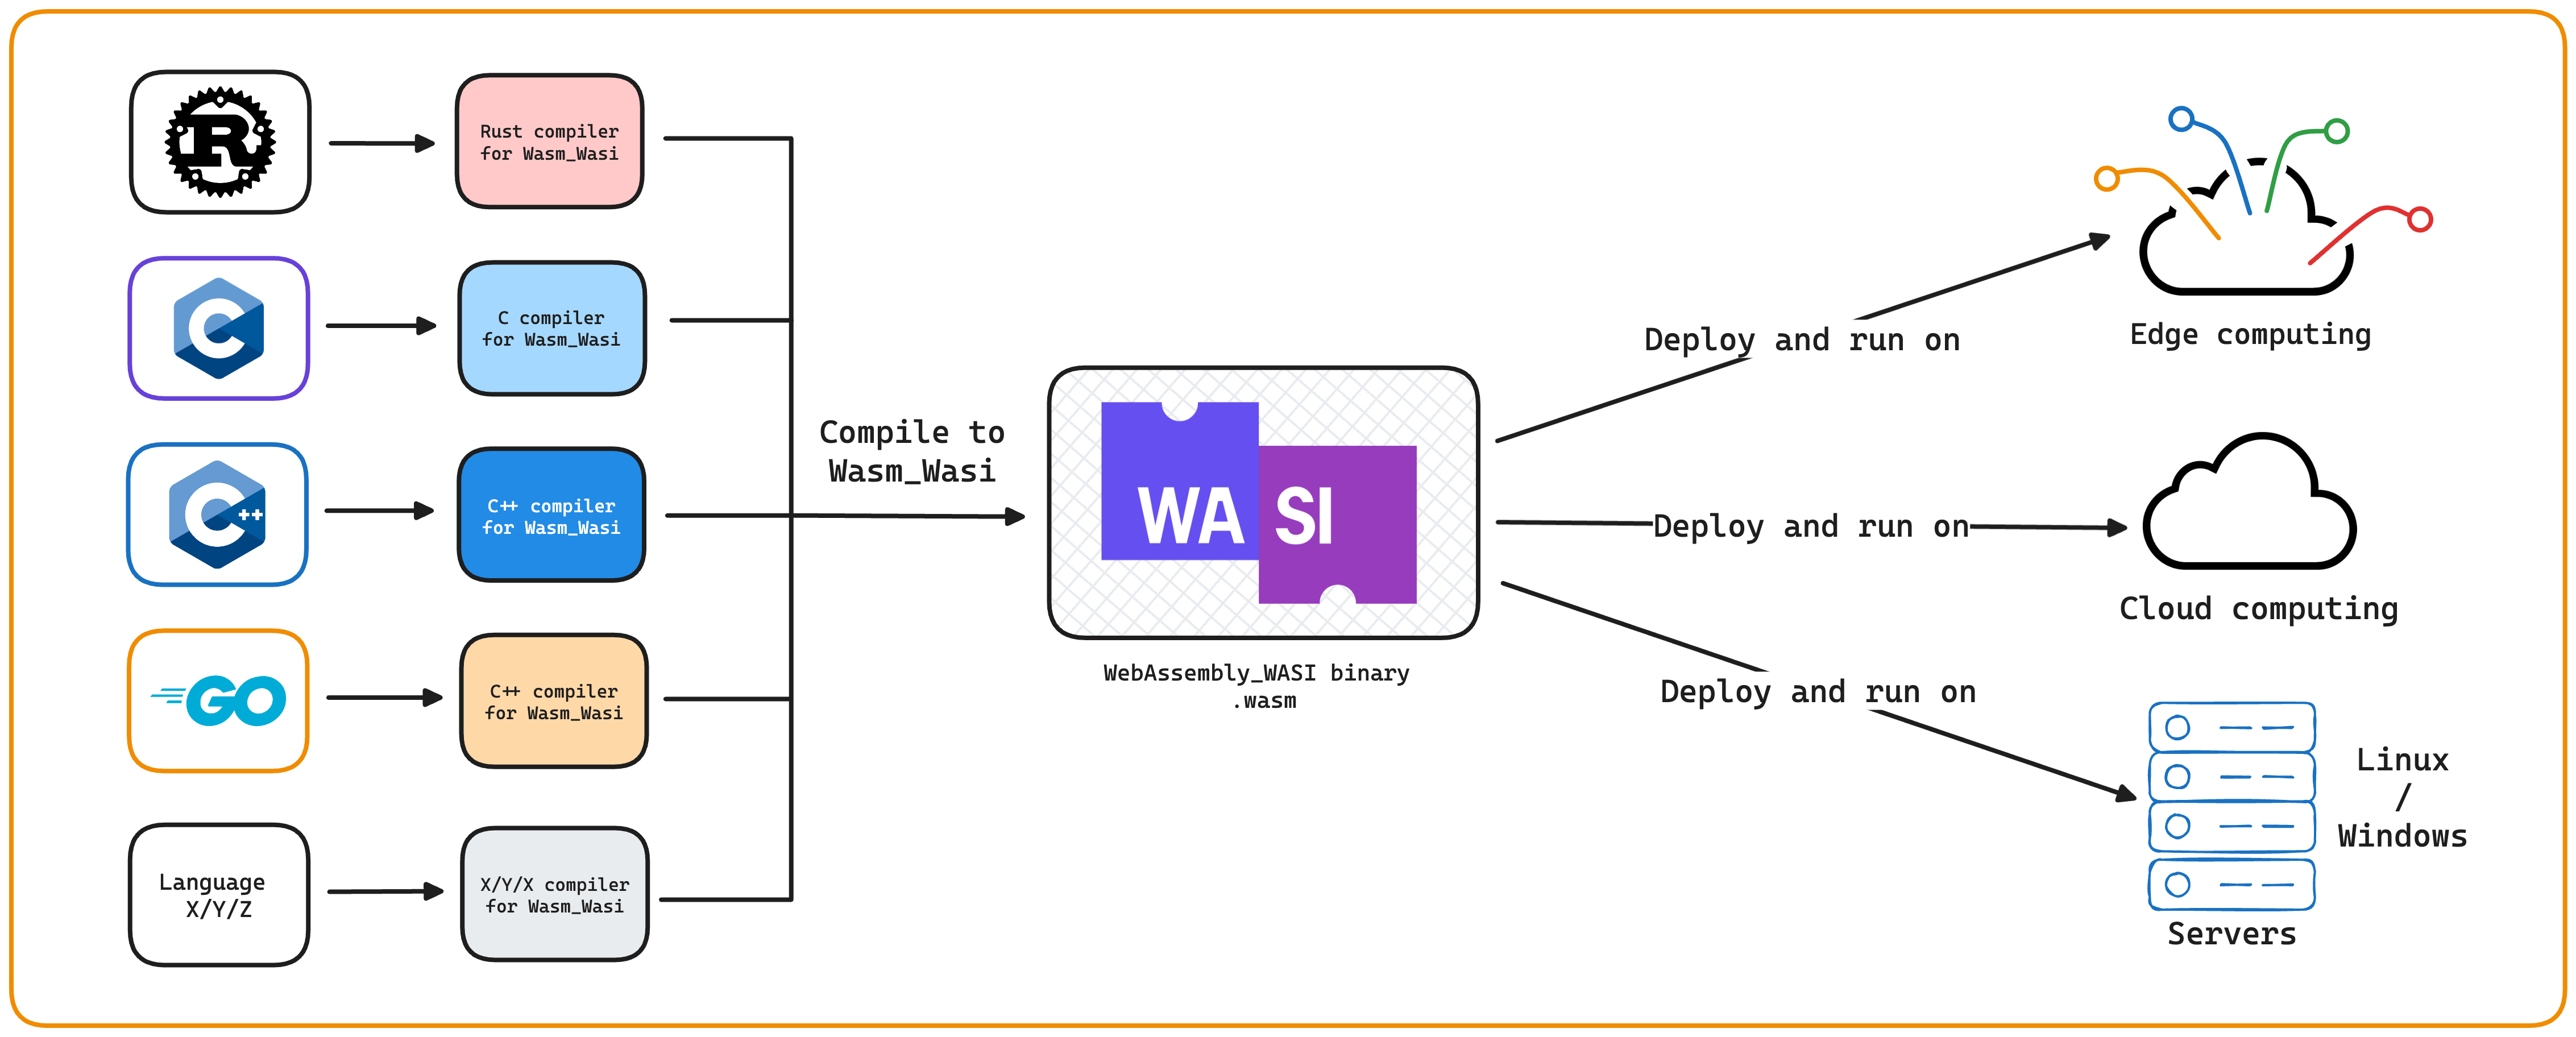
\includegraphics{assets/3-wasi-figure.png}
  \caption{Source code compiled to wasm\_wasi32 and deployed on platforms that support running the binaries.}
  \label{fig:wasm-wasi}
\end{figure}

\subsection{WebAssembly Runtimes}
\label{sect:wasm_runtimes}

WebAssembly modules cannot run independently; they require a runtime
environment to interpret and execute them. Several WebAssembly runtimes
have been developed to support the execution of WebAssembly modules in
different environments, such as Wasmtime, Wasmer, and WasmEdge
\citep{zhang2024}.

\citet{zhang2024} explains that these runtimes provide a secure and
efficient execution environment for WebAssembly modules, enabling them
to run on a wide range of platforms, including cloud servers, edge
devices, and even embedded systems. They explain that some runtimes
offer features like \ac{AOT} compilation, which can further improve the
performance of WebAssembly modules. \Cref{fig:wasm-runtimes} below
illustrates how code written in a programming languages with support for
compiling to \ac{Wasm} can run cross-platform.

\begin{figure}[H]
\centering
  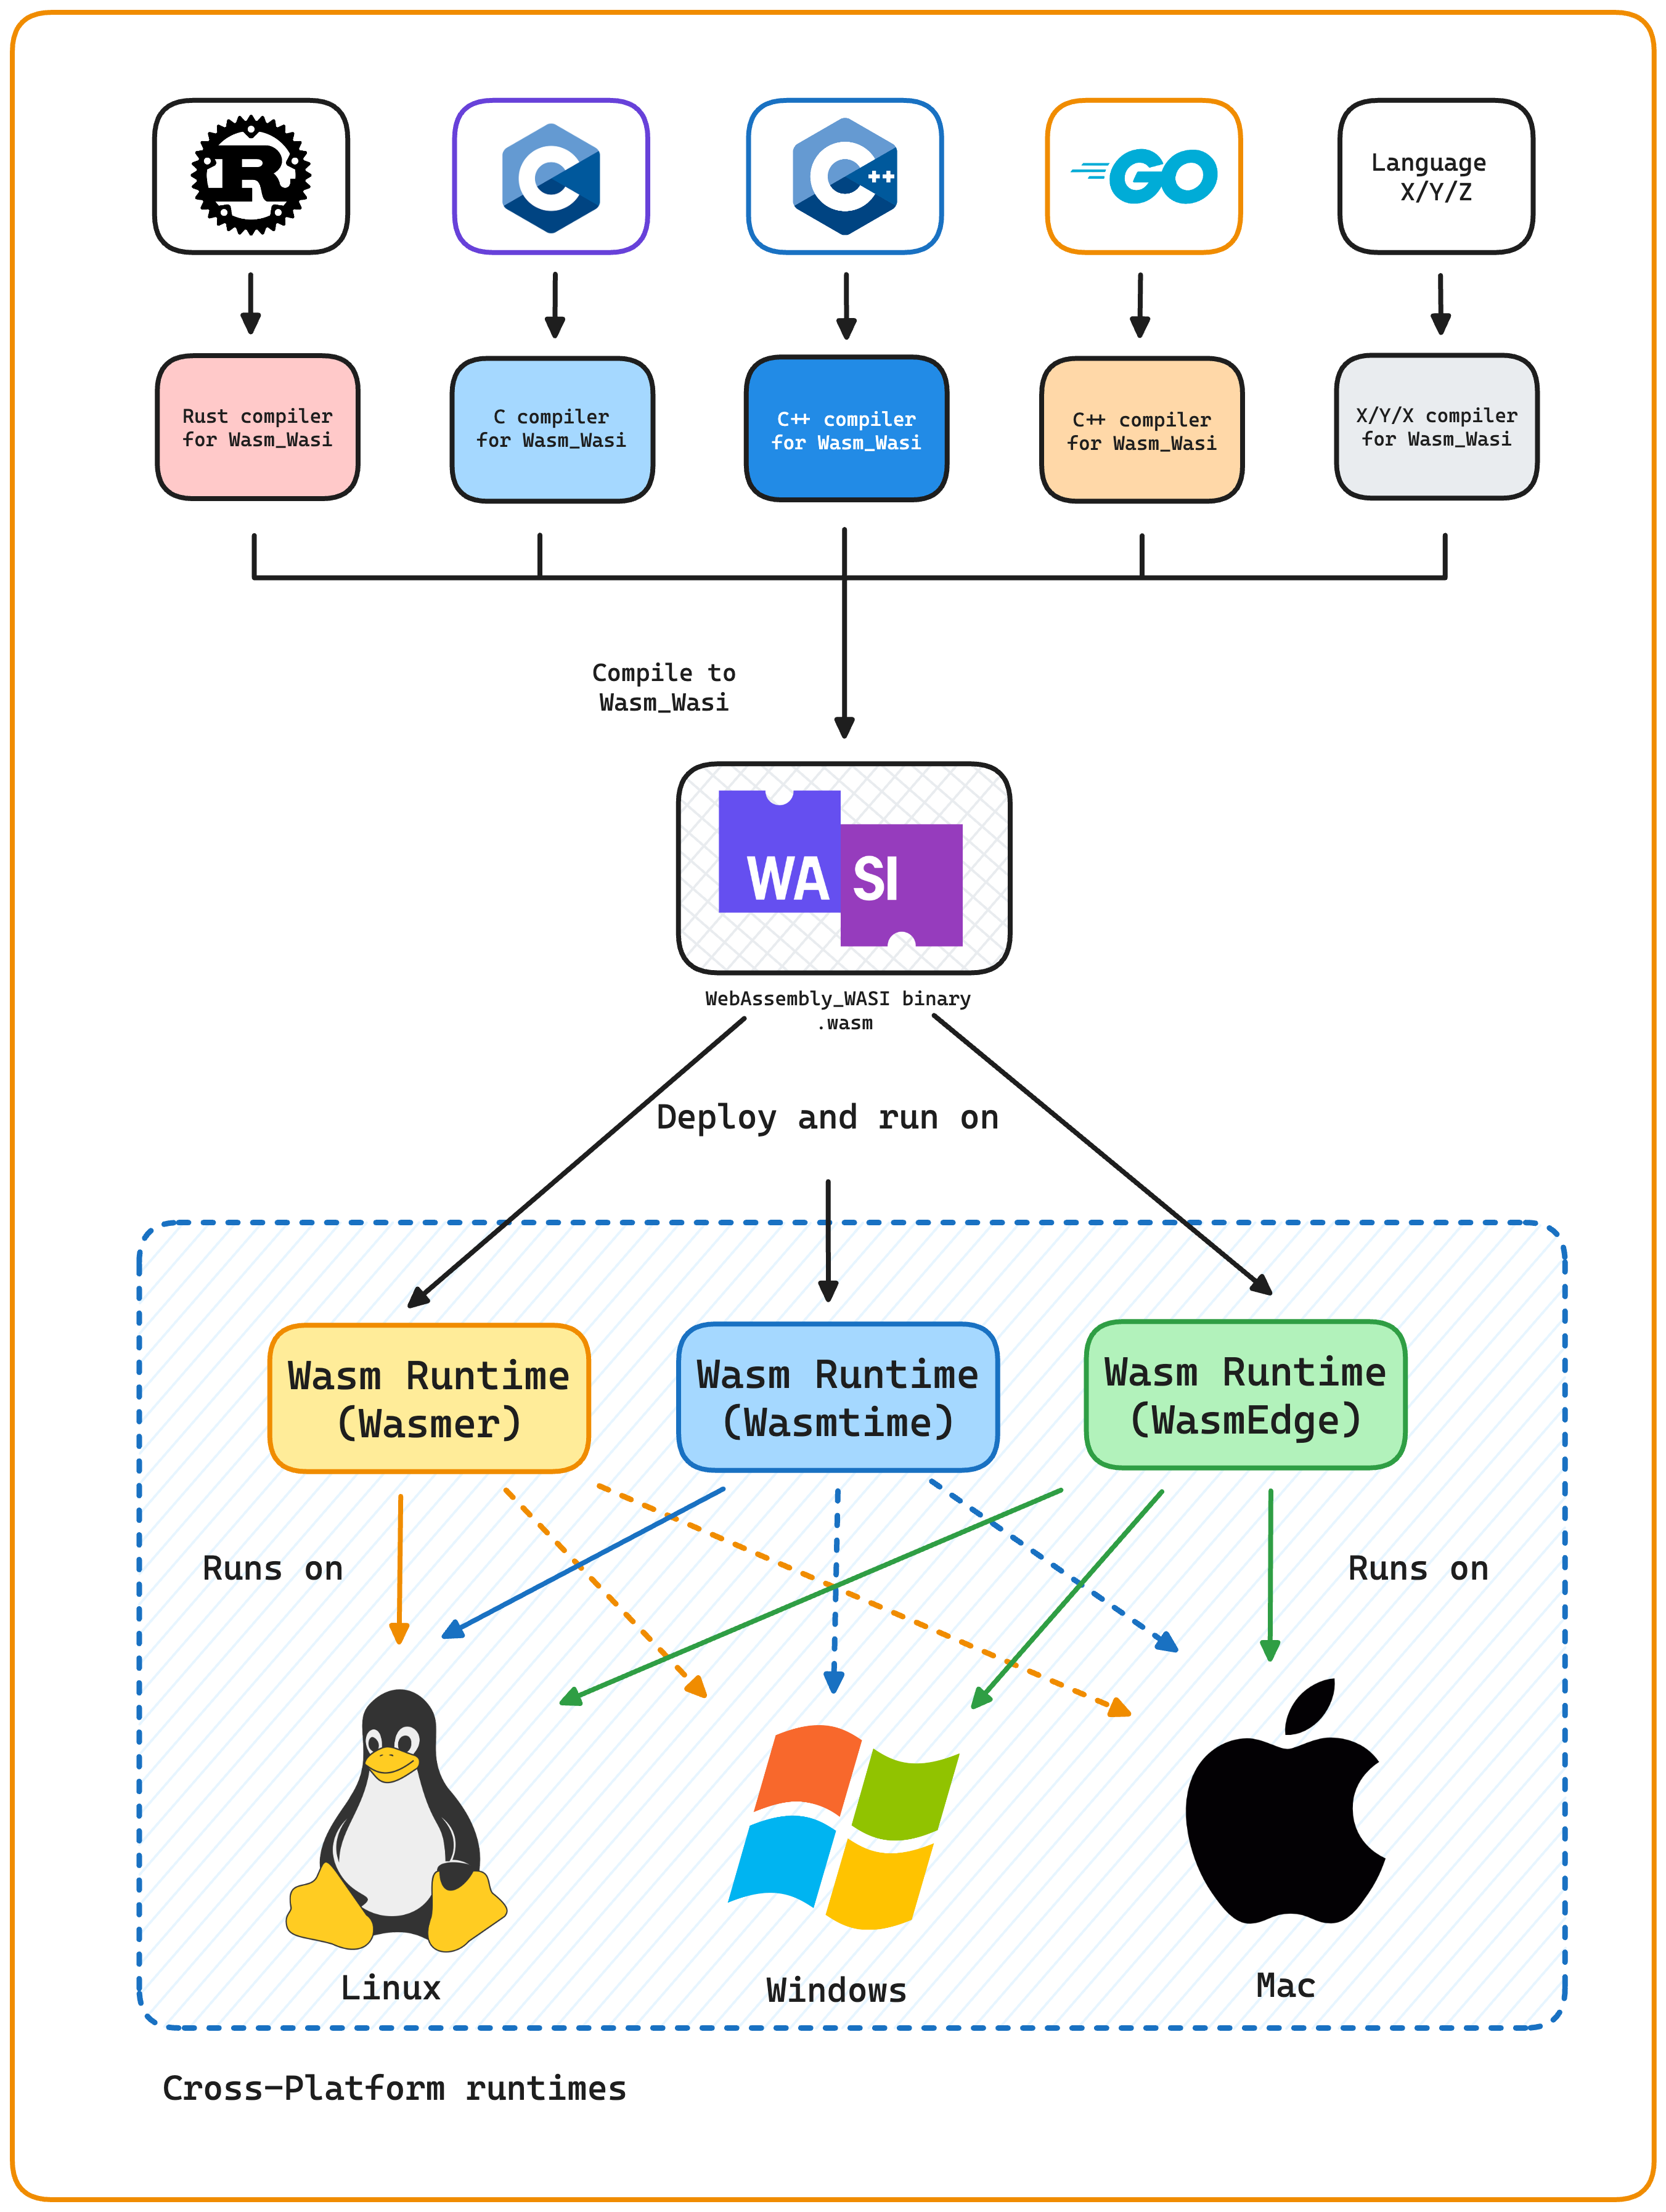
\includegraphics[width=0.7\columnwidth]{assets/3-wasm-runtime.png}
  \caption{Source code compiled to wasm\_wasi32 that can run anywhere
a WebAssembly runtime can be installed.}
  \label{fig:wasm-runtimes}
\end{figure}

The combination of WebAssembly, WASI, and efficient runtimes has sparked
interest in using WebAssembly as an alternative to traditional
containerization technologies, such as Docker, in cloud-native and
serverless environments \citep{shillakerFaasmLightweightIsolation2020a,
sebrechtsAdaptingKubernetesControllers2022}.

\section{Energy Monitoring}
\label{sect:energy_monitoring}

Monitoring and measuring energy consumption can be useful for
understanding and optimizing the energy efficiency of cloud computing
environments. Energy measurements provide insights into the impact of
different technologies, architectures, and workloads on overall energy
usage
\citep{shehabiUnitedStatesData2016, al-fuqahaInternetThingsSurvey2015}.

Several protocols and techniques have been explored to collect and
analyze energy consumption data, and this thesis will explore some of
these. These protocols enable the transmission of energy data, which can
be used for optimizing energy efficiency
\citep{al-fuqahaInternetThingsSurvey2015}.

\subsection{MQTT}

The \ac{MQTT} protocol is a lightweight and efficient protocol that has
been used for energy monitoring. In an \ac{MQTT} setup, a broker server
acts as an intermediary, facilitating communication between devices and
servers. This enables efficient data exchange between publishers and
subscribers \citep{al-fuqahaInternetThingsSurvey2015}. (See
\Cref{fig:mqtt-model.png}).

\begin{figure}[H]
\centering
  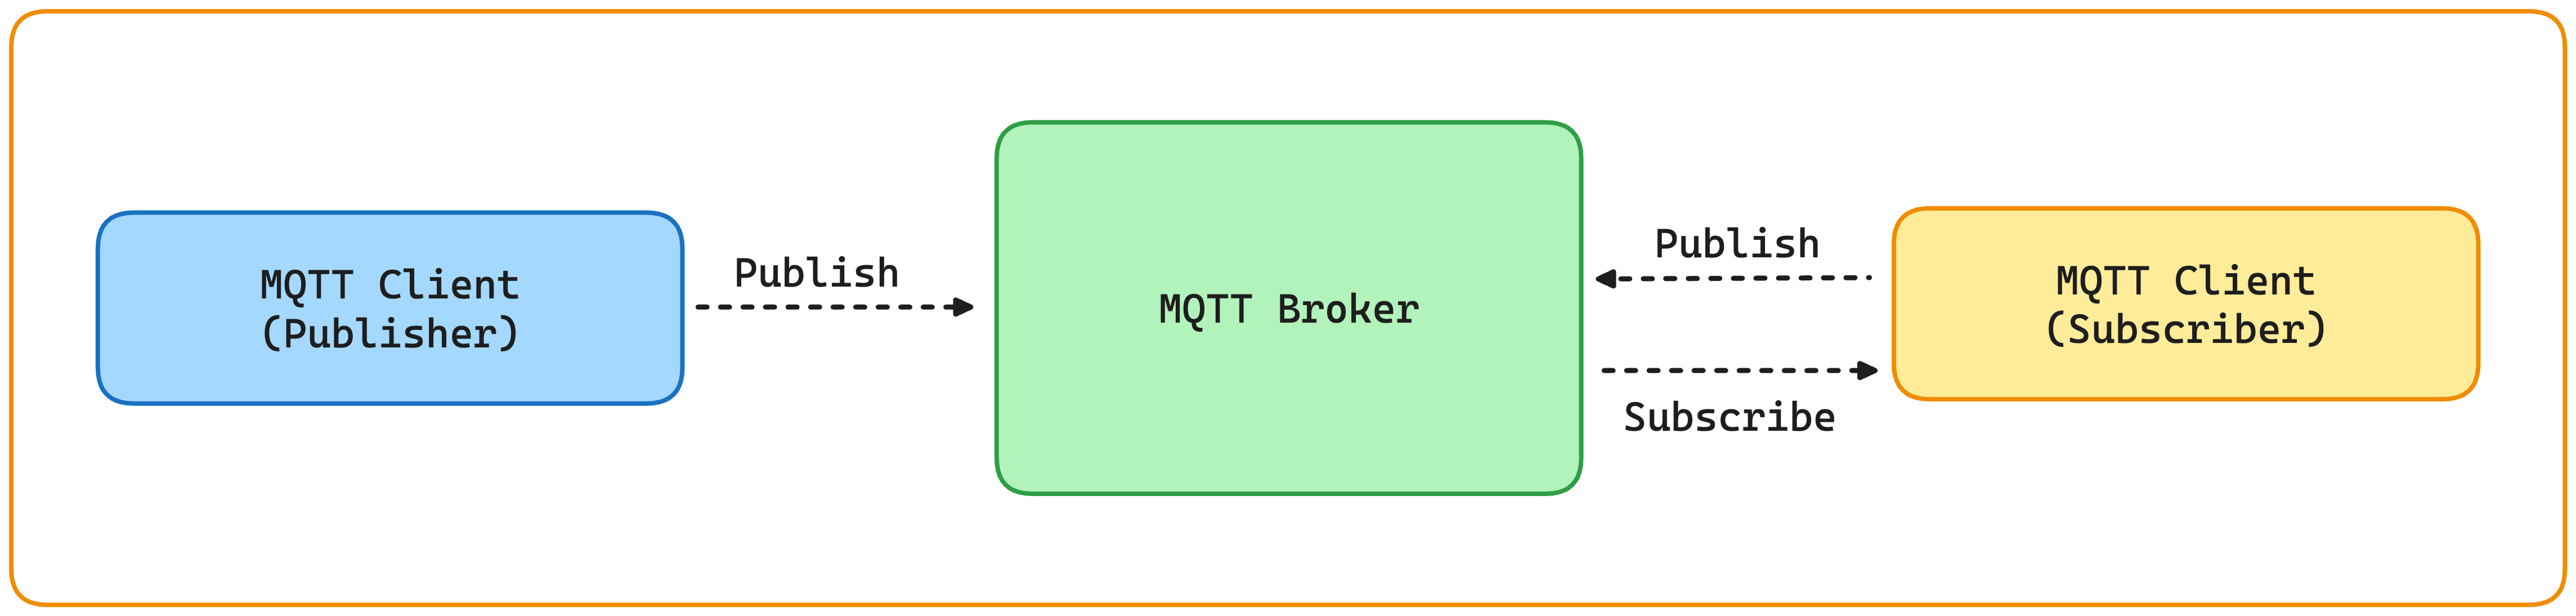
\includegraphics{assets/3-mqtt-pubsub.png}
  \caption{PubSub model of the \ac{MQTT} protocol.}
  \label{fig:mqtt-model.png}
\end{figure}

\subsection{Z-Wave}

Z-Wave is a wireless communication protocol designed for home automation
and energy management. It has been used in research studies to develop
energy monitoring systems for residential buildings, enabling monitoring
and control of energy consumption
\citep{al-fuqahaInternetThingsSurvey2015}.

\subsection{Aeotec Smart Switch}

The Aeotec Smart Switch 6 is a power switch that is primarily used for
home automation. It allows its users to integrate with it through a
Aeotec Z-Stick what communicates with the switch through Z-wave. A
supporting library; zwave-js-ui\footnote{\url{https://github.com/zwave-js/zwave-js-ui}},
which can be setup as a Docker container on a computer, can read energy
measurements from the Smart Switch at a given interval and publish the
values on a \ac{MQTT}-topic. This is in turn picked up by the \ac{MQTT}
broker and published to its subscribers. This switch supports reporting
measurements at an interval of 1 second \citep{aeotecAeotecSmartSwitch}.

\begin{figure}[H]
\centering
  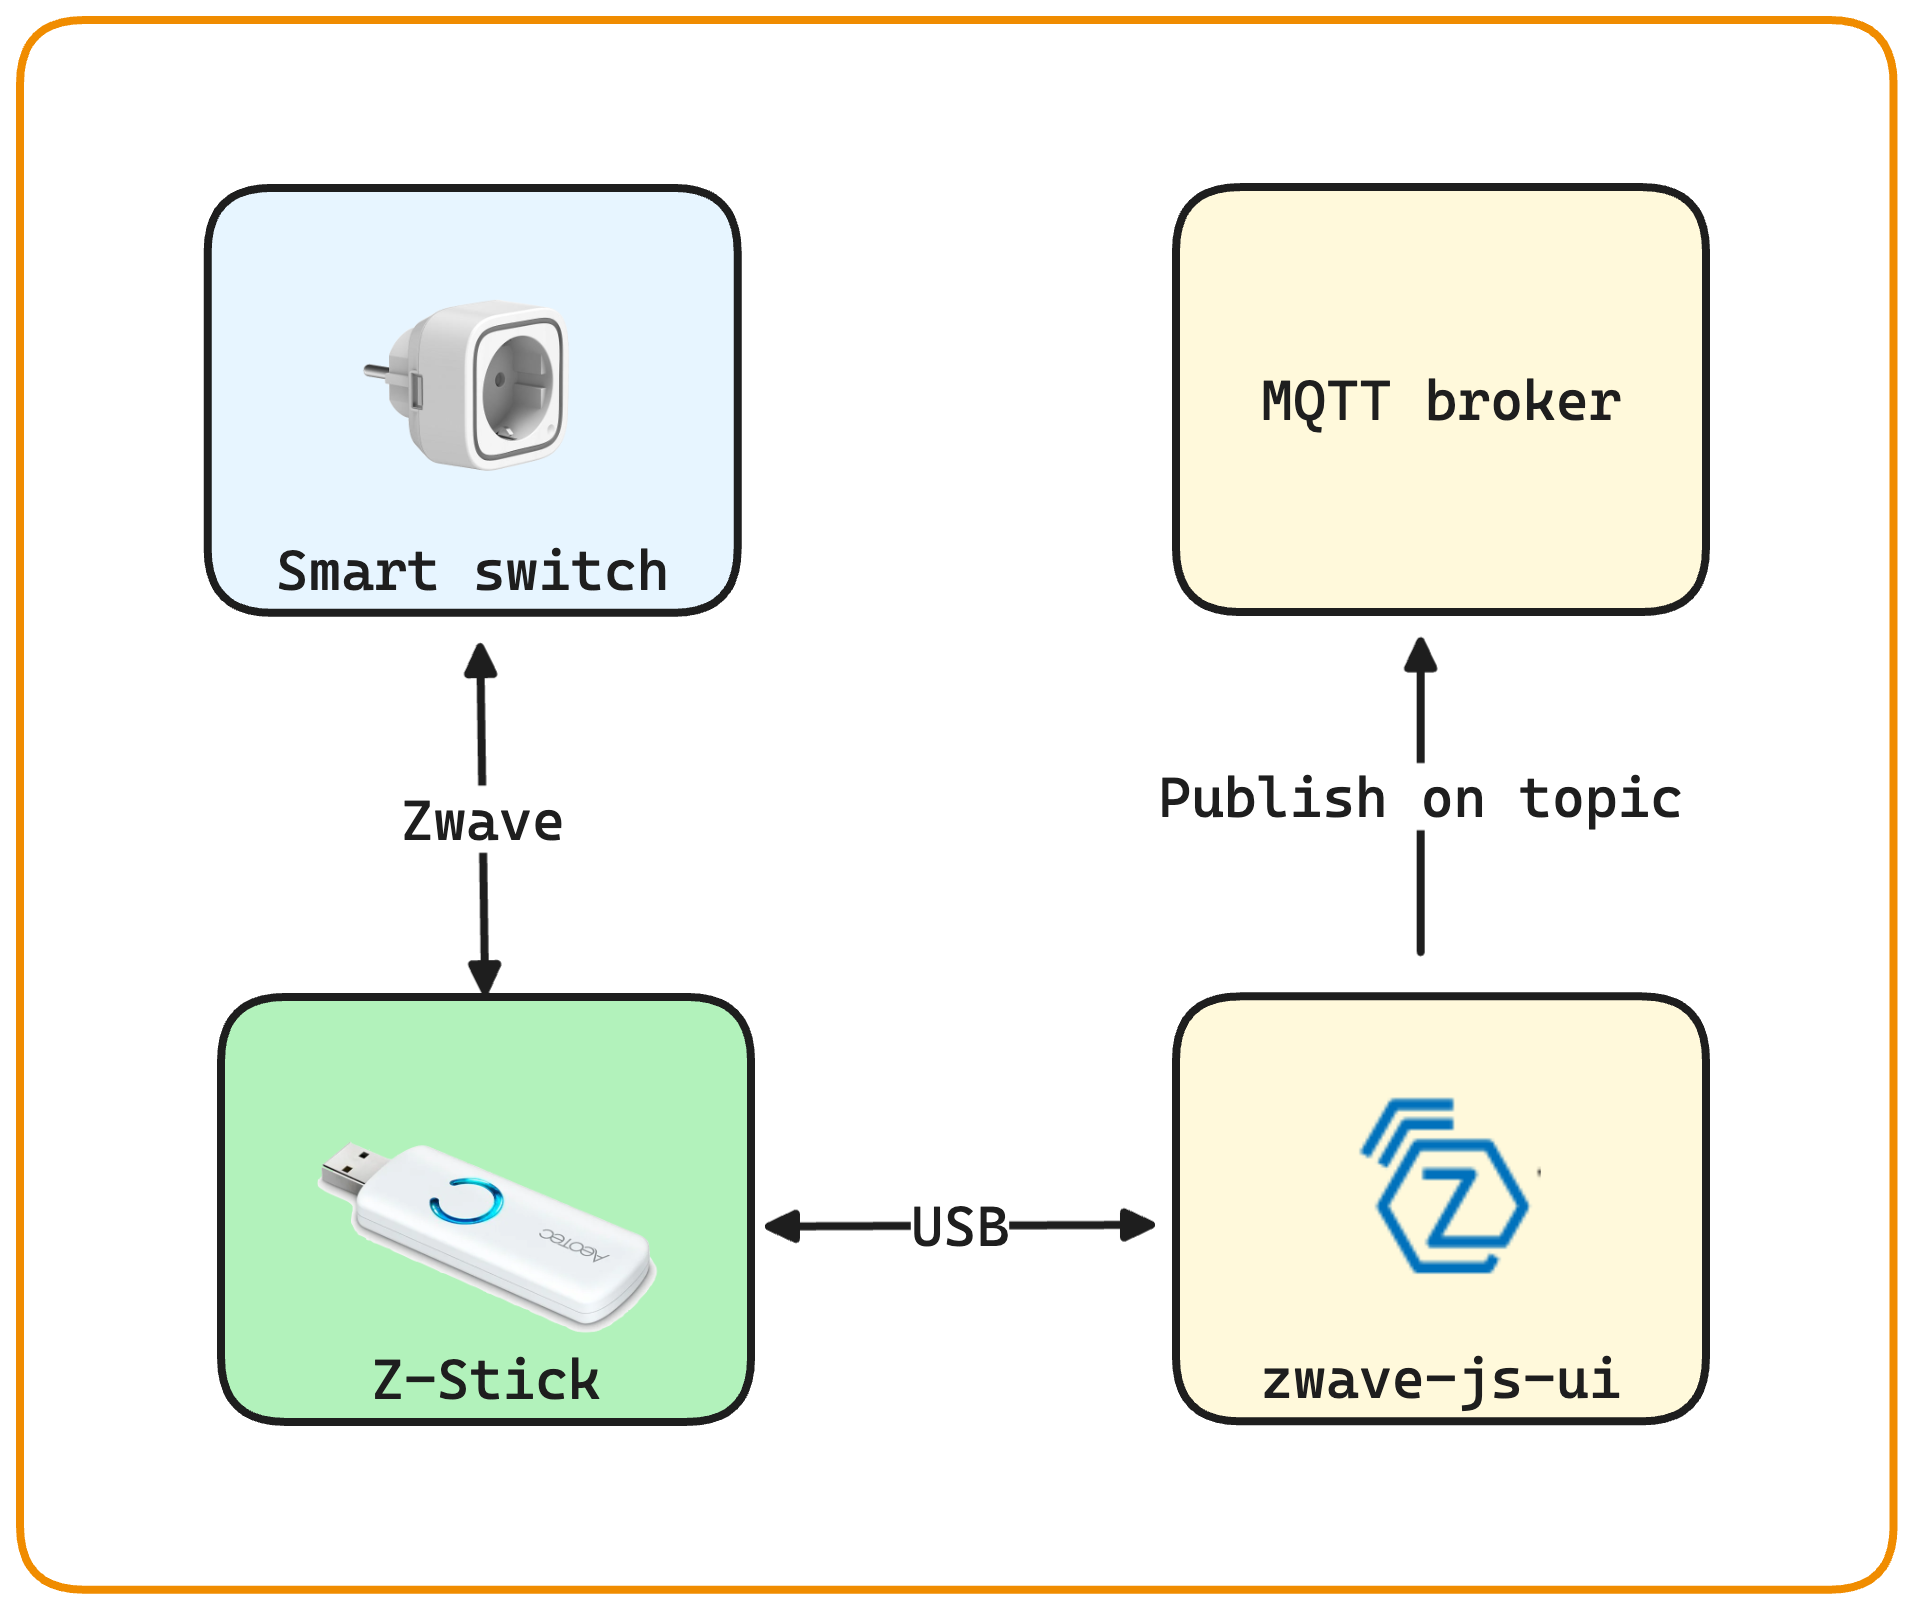
\includegraphics[width=0.7\columnwidth]{assets/3-smart-switch.png}
  \caption{Smart Switch 6 communicating with zwave-js-ui through Aeotec Smart Stick }
  \label{fig:modbus-tcp-gude}
\end{figure}

\subsection{Modbus TCP}

An alternative to reading energy measurements through a pub-sub model
with \ac{MQTT}, is to utilize the Modbus TCP protocol. Modbus TCP is a
widely adopted industrial communication protocol for exchanging data
between devices and control systems. It has been used to develop energy
monitoring and auditing systems for industrial applications,
facilitating energy audits and energy-saving strategies
\citep{tongStudyEthernetCommunication2015}. It communicates with TCP/IP
packets, and an illustration on how a client-server request and response
could look like can be found in \Cref{fig:modbus-tcp}.

\begin{figure}[H]
\centering
  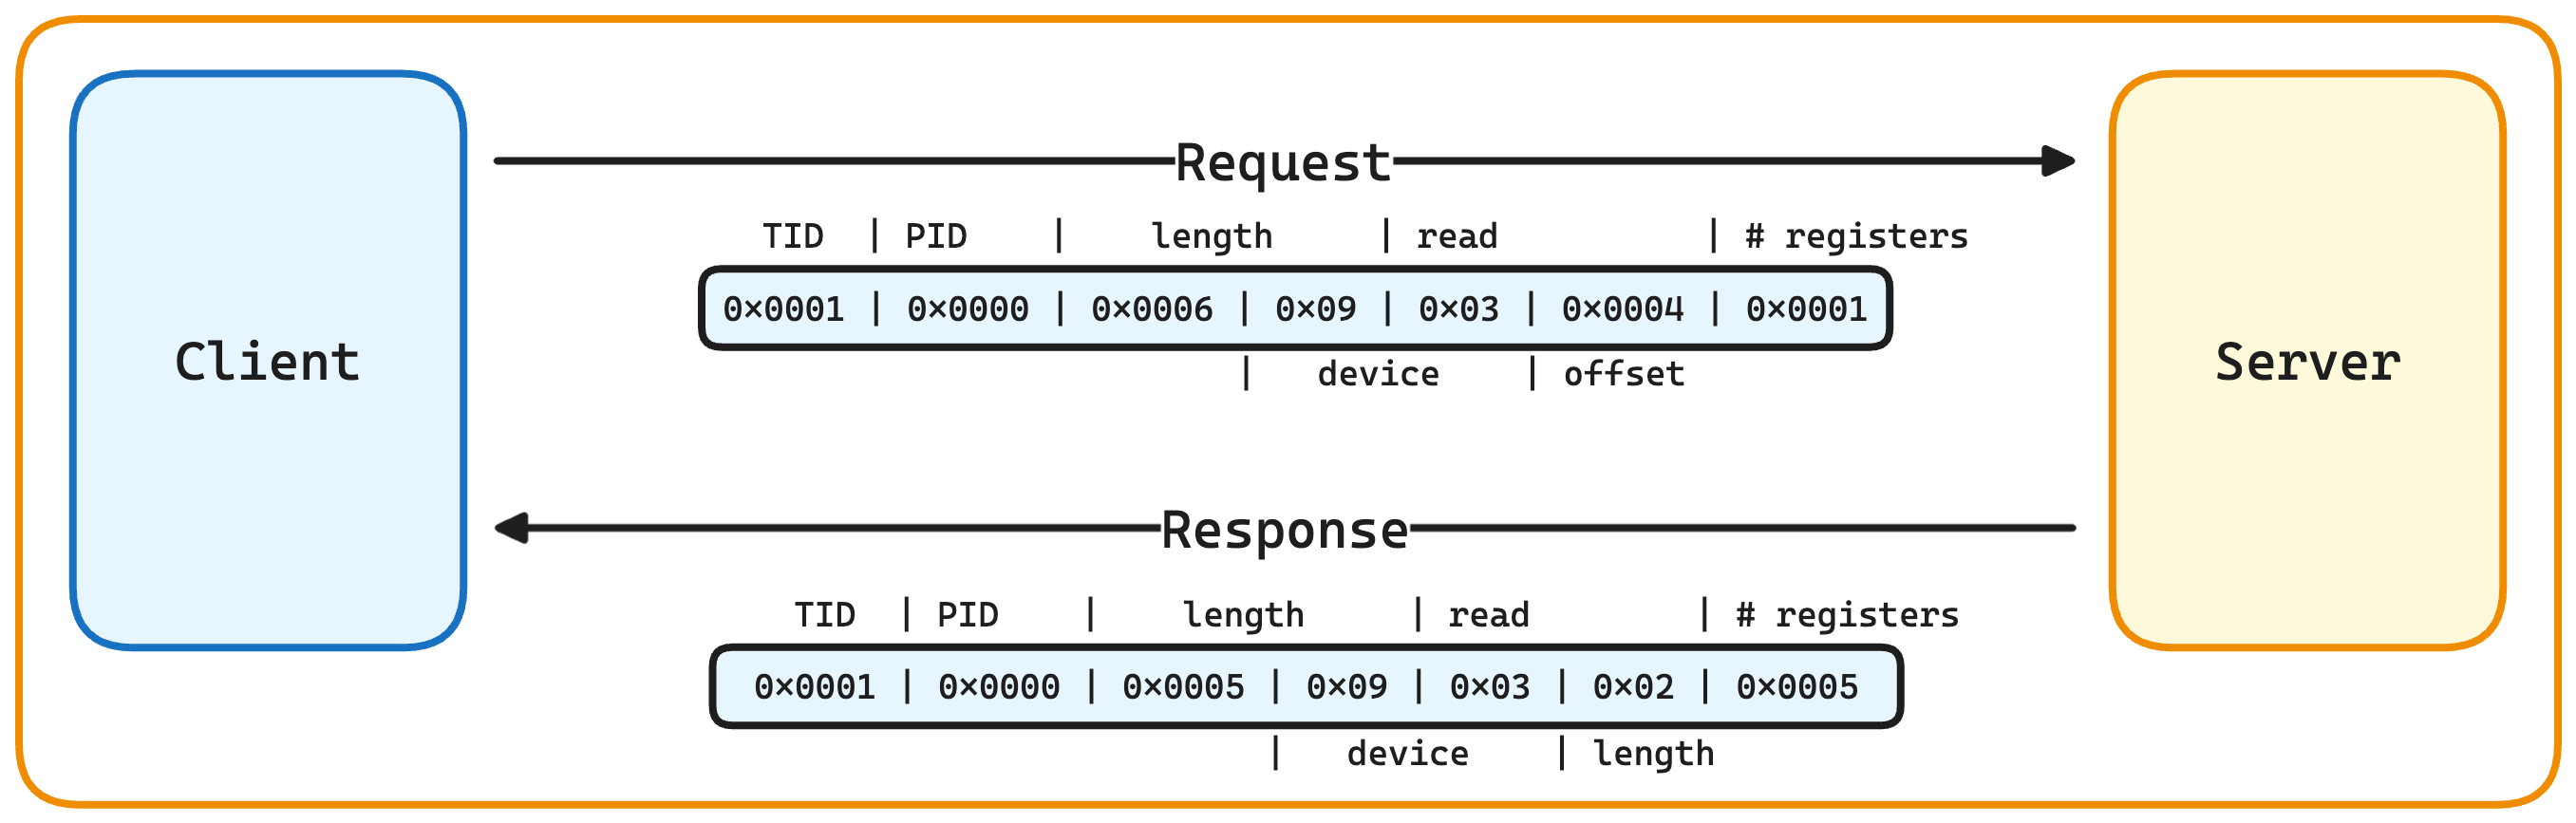
\includegraphics{assets/3-modbus-tcp.png}
  \caption{TCP/IP package exchange between a client and a server over Modbus
TCP.}
  \label{fig:modbus-tcp}
\end{figure}

\subsection{Gude Expert Power Control 1105}

The Gude Expert Power Control 1105 is a switched PDU with an integrated
current metering and monitoring that supports communicating over TCP/IP.
It is effectively a light weight server that can measure energy,
current, power factor, phase angle, voltage, and active / apparent /
reactive power. To read these measurements, the PDU supports a handful
of interfaces, such as REST API, HTTPS, SNMP, Telnet, \ac{MQTT} and
Modbus TCP \citep{gmbhExpertPowerControl2023}. In
\Cref{fig:gude-control} below, a simplified setup with the Gude acting
as the server for communicating over Modbus TCP is shown.

\begin{figure}[H]
\centering
  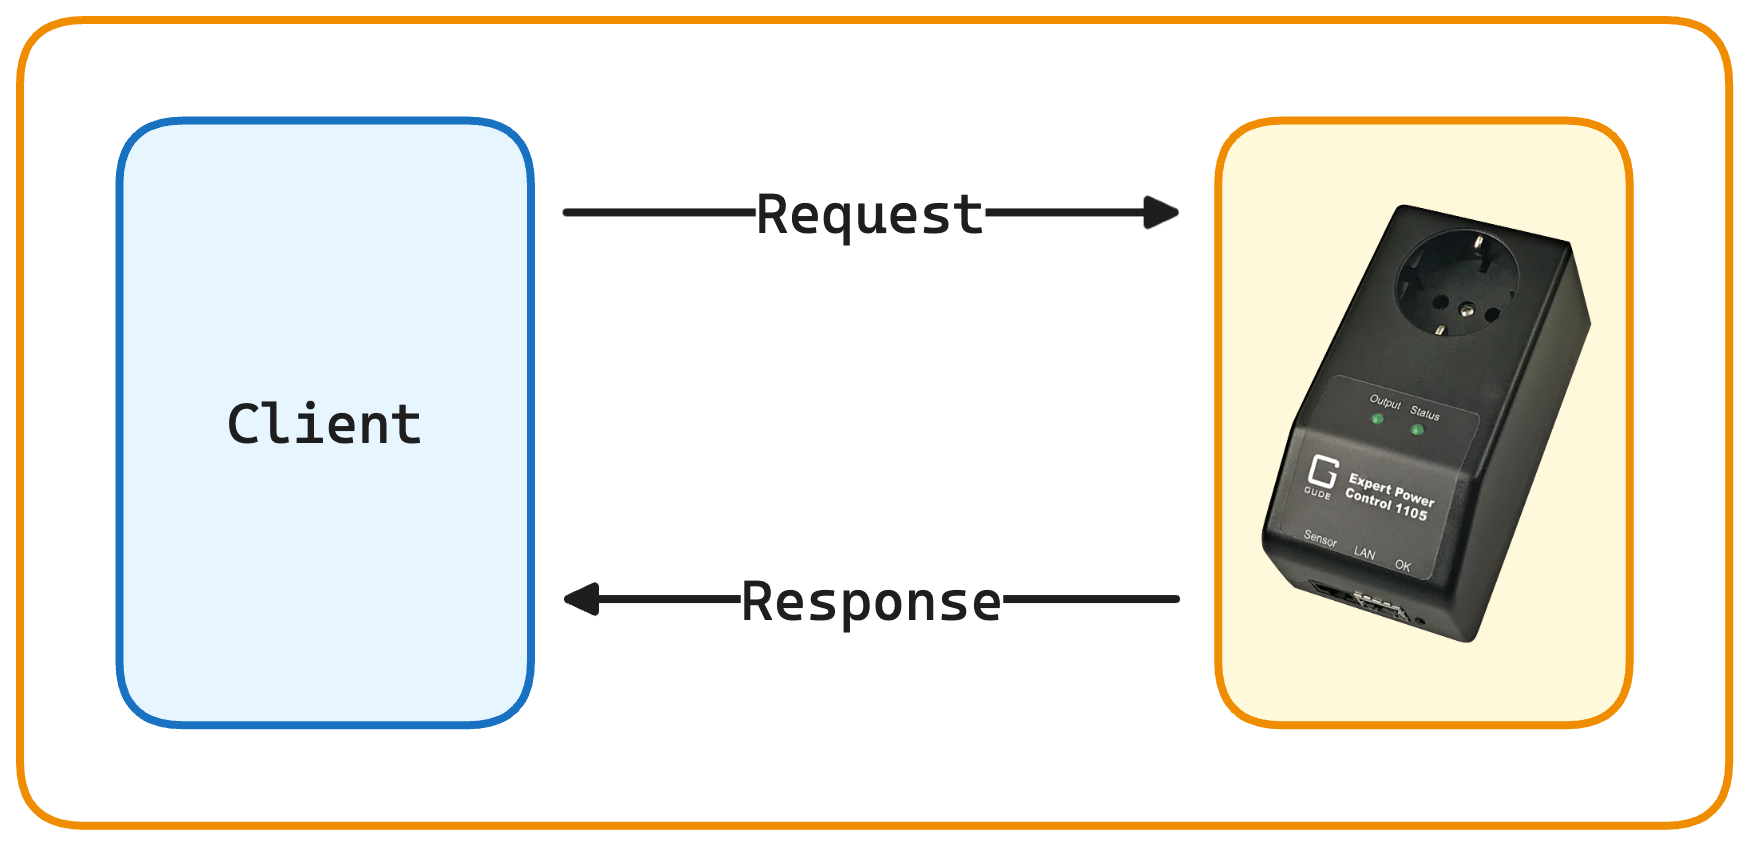
\includegraphics[width=0.7\columnwidth]{assets/3-modbus-gude.png}
  \caption{Client communicating with Gude over Modbus TCP.}
  \label{fig:gude-control}
\end{figure}

This device can measure a lot of different sensor, including current,
voltage, power draw and power factor. Voltage is the amount of volts the
system has access to, typically 240V in Norway on alternate current
(AC). The current is the amount of electricity measured in ampere that
the system is consuming. Power draw is a product of current and voltage,
\(P = U \times I)\), while Power factor is a factor between 0 to 1 that
describes the amount of power consumed that is spent on actual usage.
For example, a power factor of 0.5 means that 50\% of the power consumed
in a circuit goes to waste. Most data centers aim to get as close to a
power factor 1 as possible, to ensure the energy they pay for is spent
on actual computation \citep{rasmussenImpactLeadingPower2020}.

\part{Project}

\chapter{Methodology} 
\label{chap:method}

To reiterate, the goal of this thesis is to investigate the two problem
statements presented in \Cref{sect:problems}. We are going to develop a
FaaS prototype, named Nebula, which we are going to use for conducting
experiments to see if the claim that \ac{Wasm} modules offer a more
efficient way to develop and deploy our cloud native applications holds
true. On this platform we are going to deploy functions written in Rust
that are either compiled to \ac{Wasm} modules or compiled to Rust
binaries that get packaged into a Docker image.

This chapter will present the intended methodology on how we will
conduct our experimental research method. We will employ an experimental
research method, where we will build a prototype, perform experiments on
it in a controlled environment, collect measurements and compare the
results.

\section{Experimental Framework}
\label{sect:exp_frame}

The main focus of this thesis is to build a prototype and perform
experiments on it, to measure the capabilities of \ac{Wasm} modules as a
model for deploying and running cloud applications. An experimental
approach was chosen to test the problem statements, as we can have
controlled manipulation of variables, measure the outcomes, and compare
directly between two deployment environments; \ac{Wasm} modules and
Docker containers.

We will perform a series of controlled experiments designed to measure
startup latencies (cold start), total runtime, and energy consumption
for each invocation of a function. This allows for a precise evaluation
of how \ac{Wasm} modules compare against traditional container-based
deployments in the context of cloud-native applications.

To capture energy measurements, we will need to use hardware locally
that we can control. For this we will look at the protocols mentioned in
\Cref{sect:energy_monitoring}, and use a Raspberry Pi as our local
deployment environment. We will also capture startup and runtime data on
these invocations, but not many cloud applications today are deployed on
Raspberry Pi's, so we will also need to deploy Nebula on a more typical
setup.

\subsection{Prototyping}
\label{sect:prototyping}

The prototype we are going to build for this project will be named
Nebula, named after the celestial phenomenon that can be observed in the
form of a giant cloud out in space. On Nebula we will develop a way to
deploy and invoke functions in the form of \ac{Wasm} modules or as spun
up Docker containers. To perform the desired experiments, the prototype
will need to be able to deploy to both a Raspberry Pi 4b, and on a
typical machine hosted on the cloud. For this, we will be using
\ac{NREC} \todo{add citation/link}, a IaaS platform available to
students, where we can spin up a Debian virtual machine and set up a
service on a public IP address.

\subsubsection{Hardware specifications}
\label{sect:hardware_spec}

Experiments will be performed on two types of hardware:

\begin{enumerate}
\def\labelenumi{\arabic{enumi}.}
\item
  Raspberry Pi: A small \ac{SBC}s with an ARM64 architecture that can
  run flavors of Linux. This device will be used to measure energy
  consumption relative to function invocations, which it is well suited
  for, as it consumes small amounts of energy by itself, making it ideal
  for comparing power consumption under load
  \citep{bekarooPowerConsumptionRaspberry2016}.
\item
  Virtual Machine: A Debian-based VM running on an \ac{IaaS} platform
  (e.g., \ac{NREC}), to measure performance relative to how a typical
  cloud native application would perform.
\end{enumerate}

\newpage
\subsubsection{Nebula Requirements}
\label{sect:nebula_req}

Based on this, we can summarize what we need Nebula to be able to meet
these requirements.

\begin{table}[!ht]
\centering
\caption{Nebula requirements}
\begin{tabular}{@{}p{0.3\linewidth}@{\hskip\tabcolsep}p{0.6\linewidth}@{}}
\toprule
\textbf{Requirement} & \textbf{Description} \\
\midrule

\rowcolor{green!10} Function deployment & We should be able to deploy functions
to Nebula. \\

Function execution & The prototype should execute functions in response to user
invocations, either as \ac{Wasm} modules or as Docker containers.  \\

\rowcolor{blue!10} Measurement \parbox{0.9\linewidth}{capabilities} & The prototype should be able
to collect data for startup latencies, total runtime, and energy consumption for
each function invocation. \\

Portability & The prototype should be deployable on both a
Raspberry Pi for local testing and measurement, and on a Debian virtual machine
hosted on an IaaS platform (e.g., \ac{NREC}) for a more typical cloud setup. \\

\rowcolor{orange!10} Performance & The prototype should be built in such a
manner that it presents little overhead when running our functions, isolating
the resulting efficiency and energy readings to each function invocation. \\

\bottomrule
\end{tabular}
\label{table:nebula_requirements}
\end{table}

\subsection{Controlled Experimentation}
\label{sect:controleld_experimentation}

Controlled experimentation will be an important aspect of this research,
as it let us isolate and study the effects of the deployment environment
on performance and energy consumption. Various factors, such as input
parameters for the benchmark functions and hardware configurations, will
be controlled or kept constant across experiments to minimize the
influence of external factors and increase the validity and reliability
of the results.

To experiment on Nebula, we will craft a set of benchmark functions. As
the input value to these functions scale up, the computational load on
the server will increase, letting us measure the execution time across
different workloads.

\subsection{Benchmarking}
\label{sect:benchmark}

Benchmarking will be employed as a research method to evaluate the
performance of different configurations. Benchmark functions
representing various computational workloads will be implemented and
executed on both environments.

\subsection{Benchmark Functions}
\label{sect:bench_funct}

A total of four benchmarking functions will be selected for testing,
representing various computational workloads. These functions will be
written in Rust and compiled to both \ac{Wasm} modules and Rust binaries
packaged in Docker images. The selection of these functions is based on
their computational intensity and their ability to stress the CPU.

The functions we will implement are:

\begin{enumerate}
\def\labelenumi{\arabic{enumi}.}
\tightlist
\item
  \emph{Fibonacci}: This function calculates the \emph{nth} Fibonacci
  number in the sequence, following the formula:
  \(F_n = F_{n-1} + F_{n-2}\).
\item
  \emph{Exponential}: This function calculates the value of Euler's
  number raised to the nth power, following the formula: \(F_n = e^n\).
  This benchmark tests the performance of the prototype in handling
  intesive floating-point calculations.
\item
  \emph{Factorial}: This function calculates the sum of the factorial of
  \emph{n}, following the formula: \(n! = \prod_{k=1}^n k\).
\item
  \emph{Prime number}: This function finds the nth prime number. While
  it is harder to represent this in a mathematical formula, a
  brute-force approach will be used to stress the CPU and emulate a more
  typical scenario. The function will loop through a range of numbers (0
  through \(2^{64} - 1\)), check if the number is a prime number, and
  append prime numbers to a list until the nth prime number is found.
\end{enumerate}

By implementing, deploying and executing these functions as both
\ac{Wasm} modules and Docker containers, the research aims to provide a
thorough evaluation of the performance and efficiency of each
environment.

\subsection{Measurement and Data Collection}
\label{sect:measure_data_collect}

To quantify the efficiency and energy consumption associated with
function invocations on each environment, measurement techniques will be
employed. We will deploy Nebula, along with the \ac{Wasm} modules and
Docker images, to our target computers. For measuring startup and
runtimes of each function like a typical setup, we will deploy Nebula
and the functions to a virtual machine running Debian on \ac{NREC}.
While a Raspberry Pi 4 will serve as our deployment target for measuring
startup latencies and runtimes of a device more akin to embedded
systems, but more importantly, allowing us to measure energy consumption
on a controlled device.

The Raspberry Pi will be connected to a power supply that can report
energy readings, enabling the collection of energy consumption data
during function execution. See \Cref{fig:benchmark-setup} below for a
rough sketch on how we will set up benchmarking and energy measurements
for our experiments.

\begin{figure}[H]
\centering
  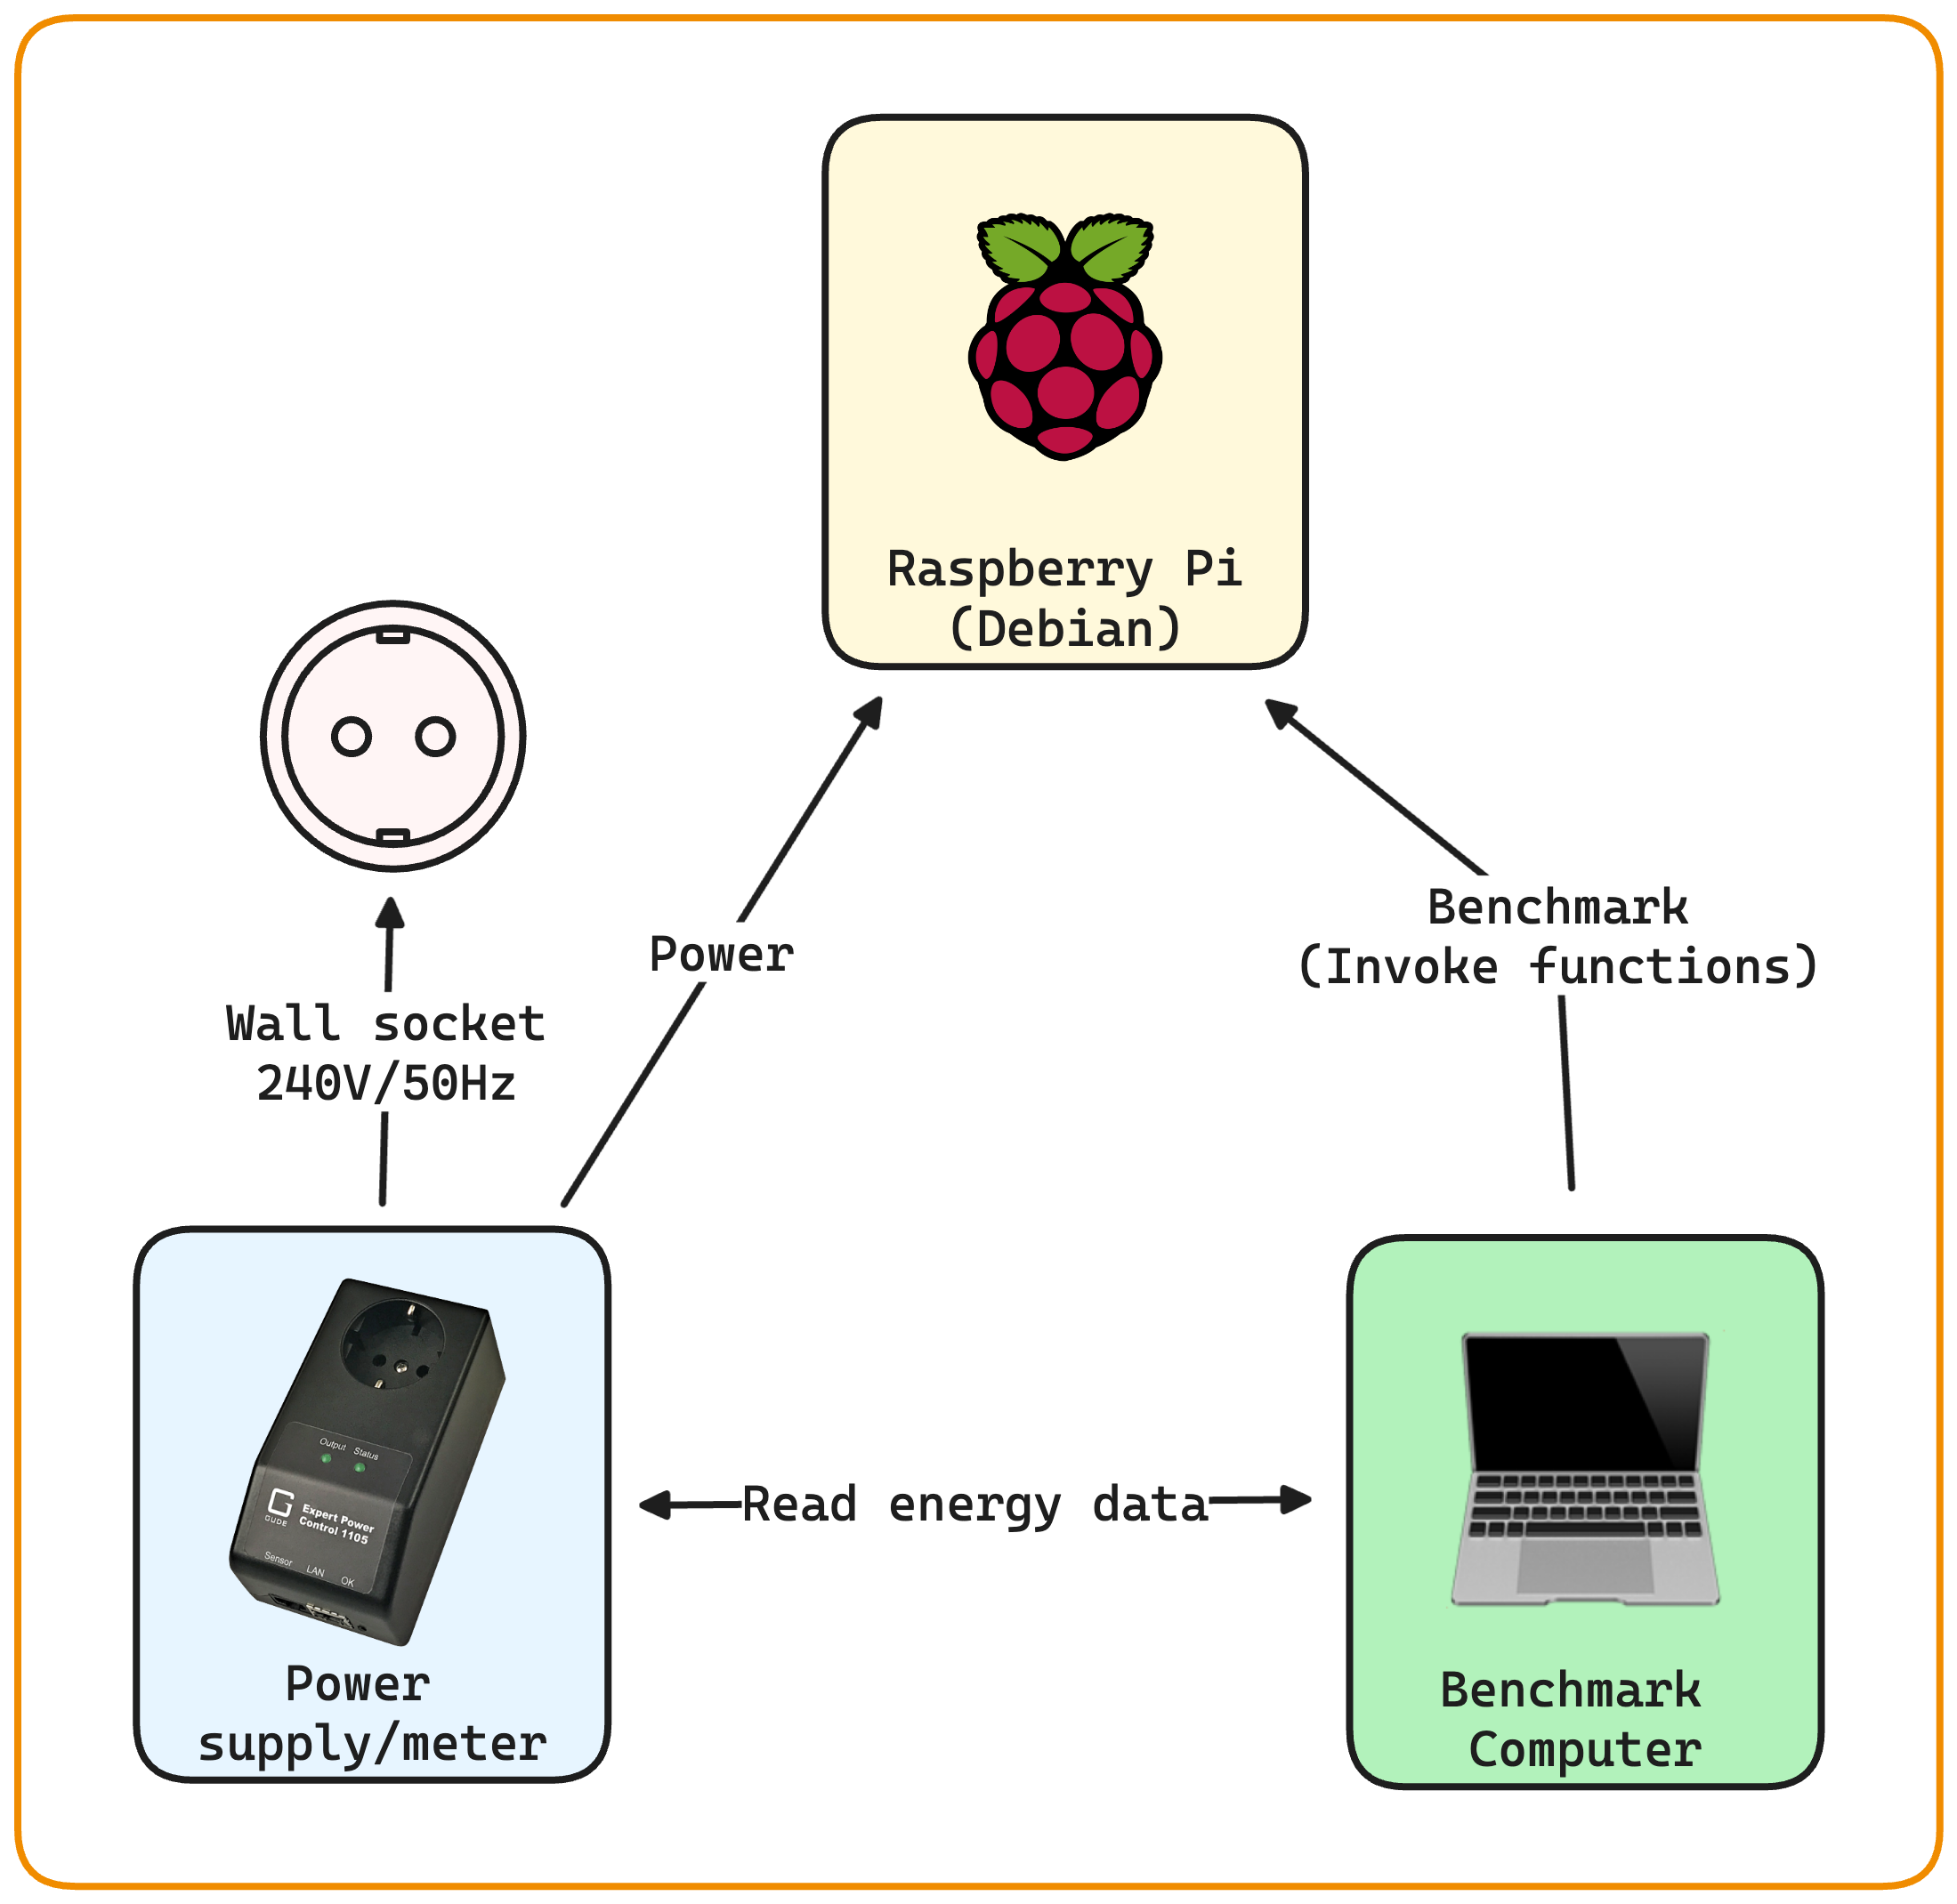
\includegraphics[width=0.7\columnwidth]{assets/4-benchmark-setup.png}
  \caption{Reading energy consumption of our Raspberry Pi.}
  \label{fig:benchmark-setup}
\end{figure}

Throughout the experiments, we will collect various data points to
evaluate the performance and energy efficiency of both \ac{Wasm} modules
and Docker containers.

To isolate how much power our functions invoke on top of the idle load
of the underlying system that hosts Nebula, we will also benchmark a
baseline power level, to measure how much power Nebula consumes while
idle. Any power consumed above this should then reflect how much power
each function invokes when called.

The following measurements will be recorded on both hardware
configurations:

\begin{itemize}
\item
  Startup latency / Cold start: For each function invocation, the time
  taken from the intial request is received until the function start
  executing will be measured. This startup latency, known as cold start,
  is a critical metric for evaluating the responsiveness and scalability
  of serverless function deployments.
\item
  Total runtime: The total execution time of each function will be
  measured, from the same time we start measuring cold start until the
  function returns the result will be measured. This metric will let us
  compare the computational efficiency of each environment under
  different workloads.
\end{itemize}

Additionally, the following measurements will be gathered on the
Raspberry Pi system system, as shown in \Cref{fig:benchmark-setup}:

\begin{itemize}
\item
  Power consumption: During the function execution on the Raspberry Pi,
  we will measure the power the server consumes at regular intervals. To
  get a more accurate reading, we will measure the current (\emph{I}) in
  \emph{mA} and the power factor (\emph{PF}), while assuming the voltage
  (\emph{U}) is a constant 240V. Using these numbers we will calculate
  the power with the following equation: \[P = U \times I \times
  PF\] Two sets of power consumption data will be collected.

  \begin{itemize}
  \tightlist
  \item
    Average Power: The average power consumption of the Raspberry Pi
    device, including any background processes, including Nebula, or
    idle draw, while invoking a function. This will be an estimation
    based on energy readings measured during the lifetime of each
    function, and calculating the average of these. We will turn off
    wifi, bluetooth and hdmi on our device to minimize external factors
    that typically draw extra power.
  \end{itemize}
\item
  Energy Consumption: Based on the power consumption measurements and
  the total runtime durations, the energy consumption for each function
  invocation will be calculated. We will calculate the energy
  consumption with the following formula:
  \[E_{\text{Wh}} = P_W \times t_h\] Two sets of energy consumption
  values will be derived:

  \begin{itemize}
  \tightlist
  \item
    Energy consumption: The total energy in \emph{Wh} consumed of the
    entire Raspberry Pi device during function execution.
  \end{itemize}
\end{itemize}

This data will then be saved in a JSON format and used for analysis.

\subsection{Data Analysis}
\label{sect:data_anal}

The collected data on startup latency, total runtime, power load and
energy consumption will be analyzed using statistical techniques to
identify patterns, trends, and potential correlations. Visualization
techniques, including line graphs, scatter plots, and bar charts, will
be used to present the data effectively and make it easy to interpret
the data. These visual representations will make it easier for us to
identify relationships between the metrics, such as impact of input size
on runtime and energy consumption.

\subsection{Comparative Analysis}
\label{sect:comp_anal}

A comparative analysis will be performed to evaluate the differences in
performance and energy efficiency between Wasm modules and Docker
containers. The following comparisons will be made:

\begin{itemize}
\item
  Startup latency: The startup times (cold starts) of Wasm modules and
  Docker containers will be compared across various input sizes to
  assess the responsiveness and scalability of each deployment method.
\item
  Total runtime: The total execution times of functions deployed as Wasm
  modules and Docker containers will be compared to evaluate their
  computational efficiency under different workloads.
\item
  Power load: The average power loads during function execution will be
  compared between Wasm modules and Docker containers to identify
  potential differences in power requirements.
\item
  Energy consumption: The estimated energy consumption for each function
  invocation will be compared across Wasm modules and Docker containers
  to evaluate their relative energy efficiency.
\end{itemize}

\subsection{Reliability and Validity}

To ensure the reliability and validity of the results we will take some
measures. Controlled experimentation will be employed, where our
experiments will be conducted in a controlled environment with variables
such as hardware configurations and input parameters kept constant
across runs. This minimizes the influence of external factors on the
results.

We will replicate each experiment multiple times to ensure the
consistency and reproducibility of the findings. The data collection
process will be automated using a benchmarking utility to minimize human
error and ensure consistent measurement techniques across all
experiments.

The results obtained from this research will be compared with findings
from existing studies in the field to help validate the observations
made in this study.

By implementing controlled experimentation, replication, automation, and
comparison with existing research, the reliability and validity of the
experimental results will be enhanced. Implementing these measures will
increase our credibility and validity of our findings from this study.

\newpage

\chapter{Designing Nebula}
\label{chap:design}

\setlength\epigraphwidth{.4\textwidth} 
\epigraph{\itshape 
The most dangerous phrase in the language is ``We have always done it this way''
}{---Grace Hopper}

Based on the requirements outlined in \Cref{sect:requirements}, we will
design a prototype named Nebula, which is a serverless \ac{FaaS}
platform capable of executing deployed functions as both \ac{Wasm}
modules and Docker containers. The primary goal of Nebula is to serve as
an experimental testbed for evaluating the performance and energy
efficiency of \ac{Wasm} modules to traditional container-based
deployments in the context of cloud-native applications. On top of this,
we will need supporting infrastructure and utilities for benchmarking
our prototype.

\section{Prototype Scope and Objectives}
\label{sect:prototype_scope}

While popular serverless platforms offered by major cloud providers are
typically closed-source, meaning how the work behind the scenes is hard
to evaluate from the outside, this prototype focuses on the aspect of
function deployment and execution of \ac{FaaS}. This controlled approach
lets us concentrate on an evaluation of deploying and runnings functions
as \ac{Wasm} modules versus Docker containers.

As a student thesis project, the prototype's scope is inherently
limited. We are not going to implement features such as automatic
scaling, distributed function deployments, authentication and
authorization, integrations with file systems and databases, and more.
However, this focused design is intentional, as we want to minimize
other factors, and rather hone in on a controlled comparison between the
two deployment methods.

\newpage

\section{System Architecture}

We will design Nebula to be a \ac{FaaS} platform that lets us execute
functions deployed as both \ac{Wasm} modules and Docker containers. The
system architecture will consist of several key components that work
together to facilitate the development, deploymend, and execution of
functions, as well as the benchmarking and evaluation of their
performance and energy efficiency.

\begin{enumerate}
\def\labelenumi{\arabic{enumi}.}
\item
  \emph{Nebula core}: The central component of the prototype,
  responsible for handling incoming requests from users, spinning up
  deployed functions, and executing them. Nebula will support both
  \ac{Wasm} modules and Docker containers, providing an interface for
  interacting with the deployed functions.
\item
  \emph{Function development and deployment}: A separate environment
  where example functions can be developed, either compiled to \ac{Wasm}
  modules or packaged into Docker images, and then uploaded to Nebula.
\item
  \emph{Infrastructure}: Two environments will be used for performing
  the experiments: a Raspberry Pi, a low-power ARM-based \ac{SBC}
  serving as the deployment target for measuring energy, and a
  Debian-based virtual machine hosted on an \ac{IaaS} platform to
  simulate a typical cloud-native application deployment environment.
\item
  \emph{Energy measurement setup}: A power supply capale of reporting
  energy readings will be used to supply the Raspberry Pi with power,
  allowing the collection of energy consumption data during function
  execution.
\item
  \emph{Benchmarking utility}: A separate benchmarking application for
  performing our experiments. We will develop this to let us create a
  benchmark suite that can be reused and test a variety of variables.
  This utility will be responsible for reading energy measurements from
  our power supply, and consolidate energy readings with function
  executions.
\end{enumerate}

\Cref{fig:system-design} illustrates the overall architecture of our
Nebula prototype system, including benchmarking and energy measurements
for our experiments.

\begin{figure}[H]
\centering
  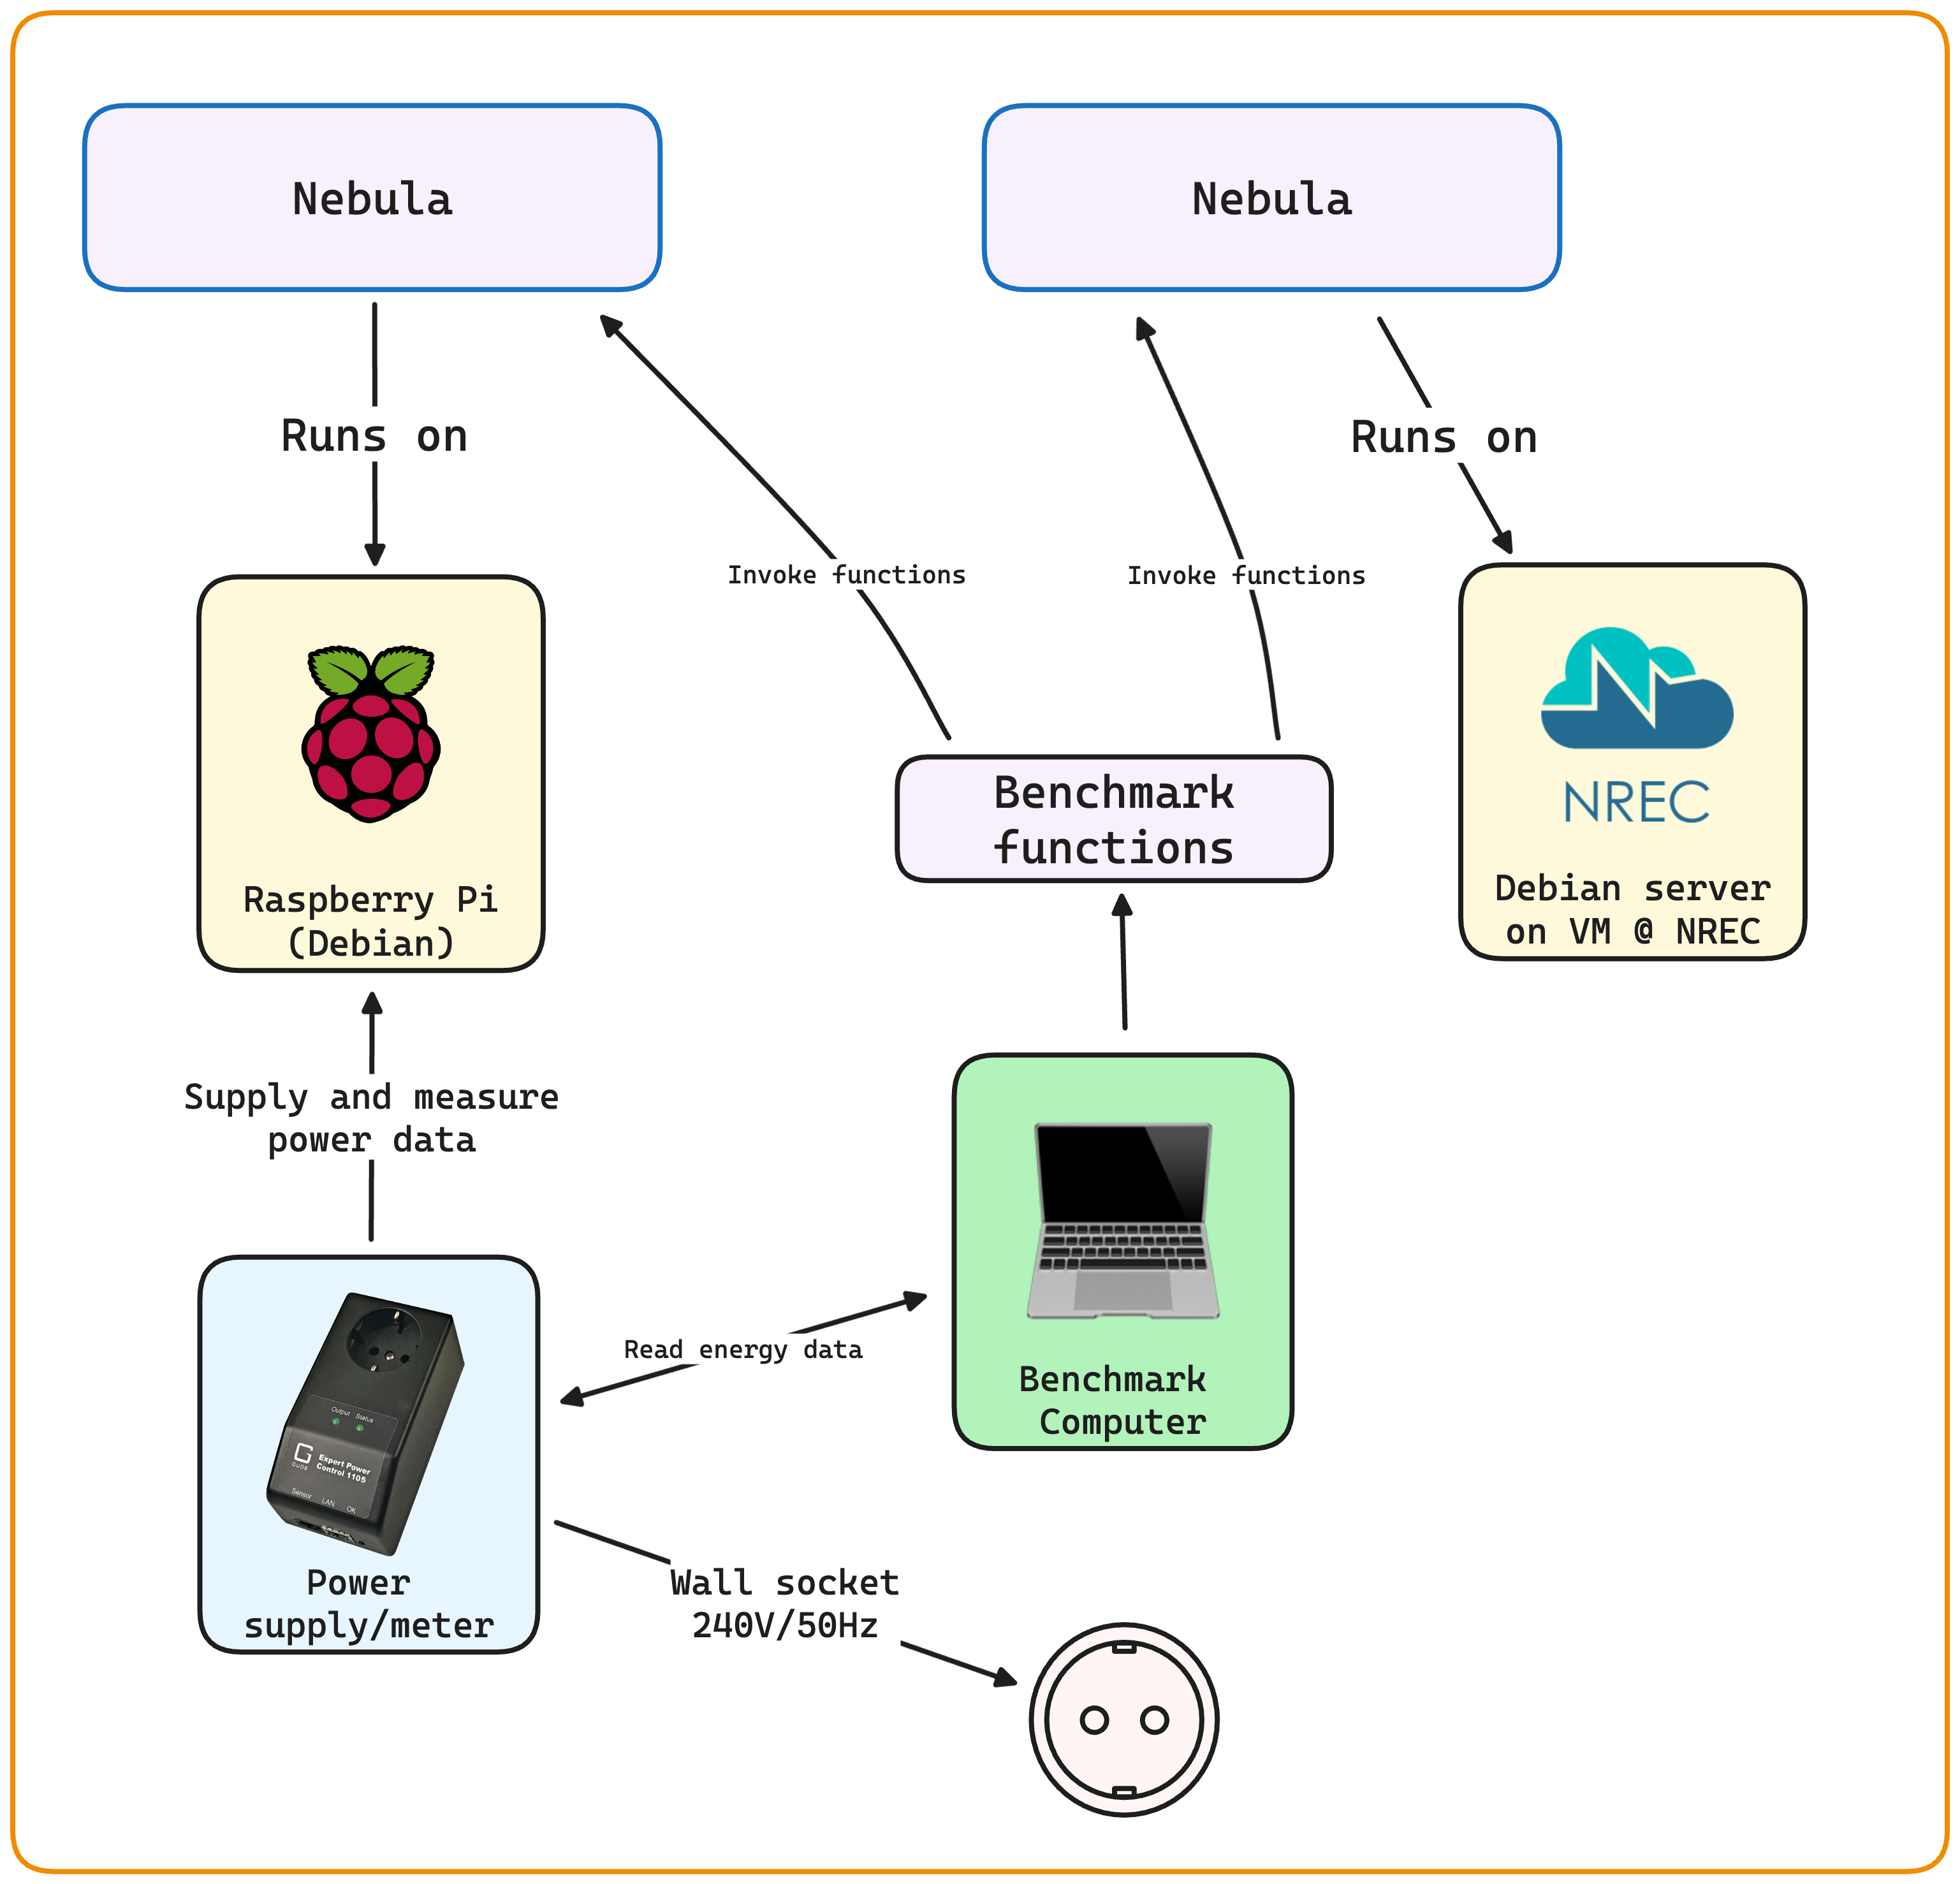
\includegraphics[width=0.7\columnwidth]{assets/5-overall-system-design.png}
  \caption{Overall architecture of our prototype system.}
  \label{fig:system-design}
\end{figure}

\section{Nebula}

Nebula will serve as the core component of the prototype. It will handle
incoming requests, manage the lifecycle of deployed functions, execute
them, and measure startup and runtimes of each execution. We will
develop an interface for users to interact with the deployed functions,
either as \ac{Wasm} modules or Docker containers.

Nebula's function execution process will involve several steps, as
illustrated in \Cref{fig:function-execution-design}. When a user invokes
a function through the interface, Nebula receives the request and routes
it to the corresponding function based on the specified deployment
method. Nebula will then start the function, execute it with the
provided input data, and return the result back to the user.

\begin{figure}[H]
\centering
  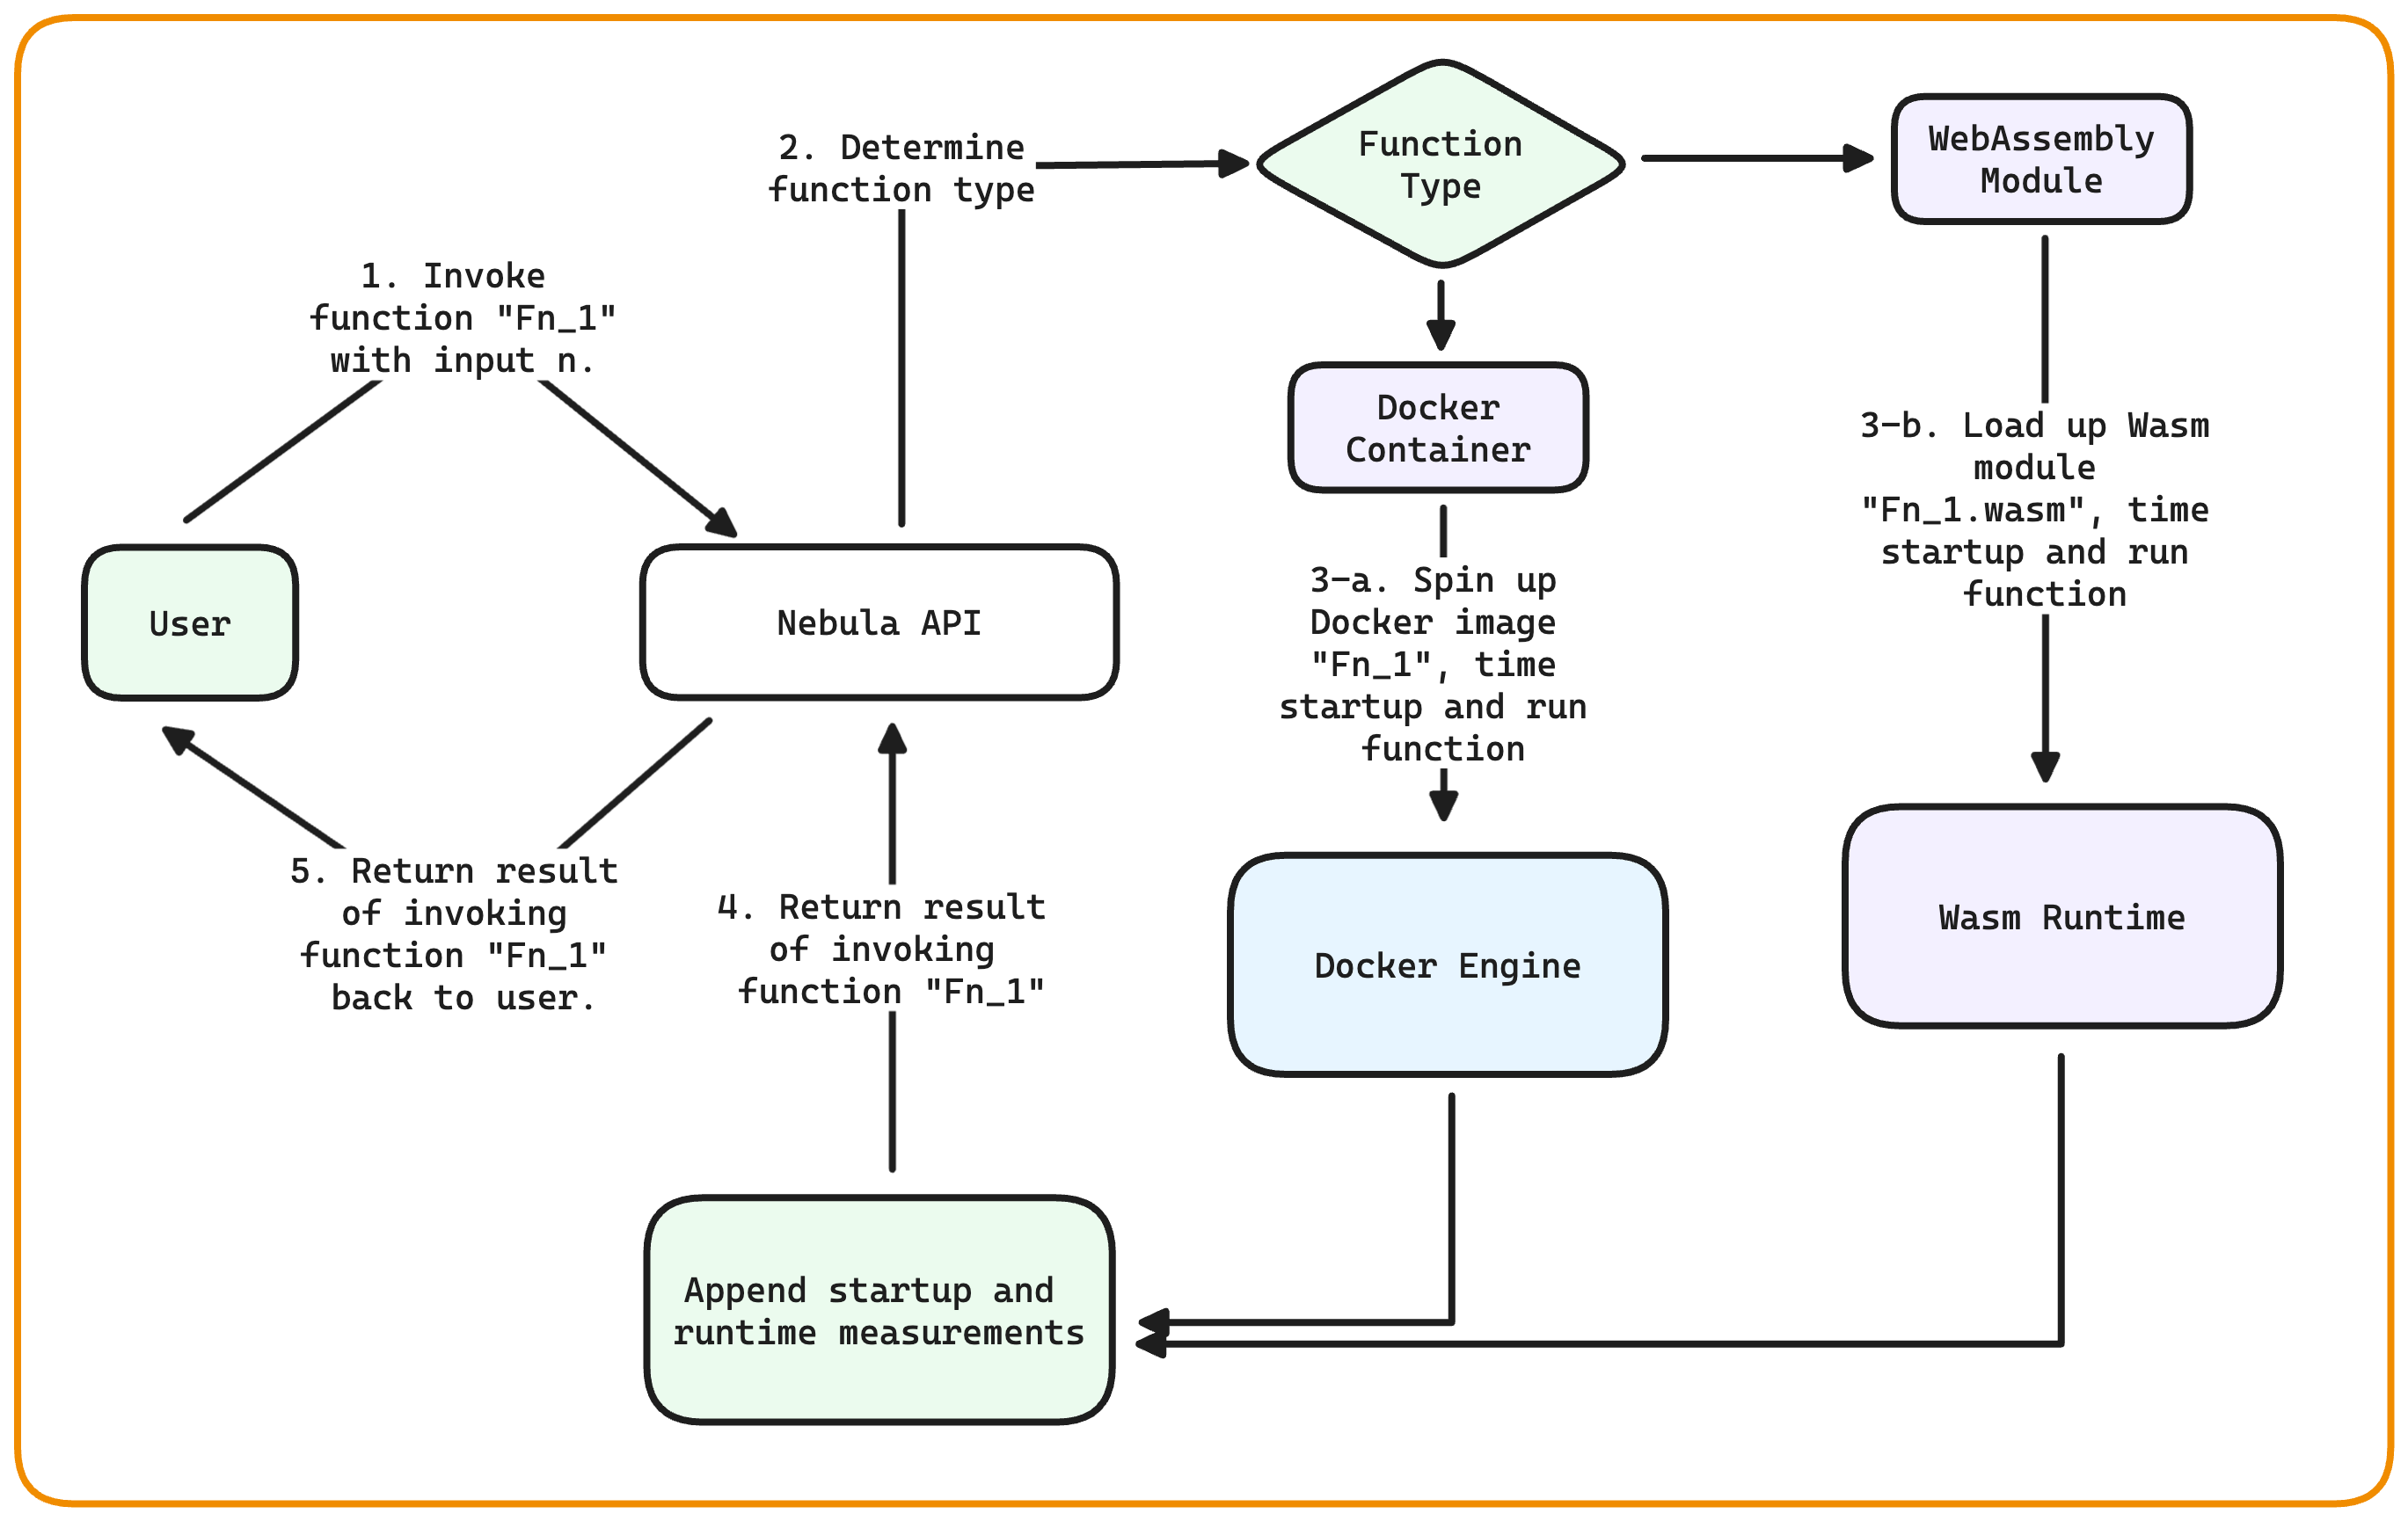
\includegraphics{assets/5-nebula-function-execution.png}
  \caption{Flow of a user invoking a function on Nebula.}
  \label{fig:function-exeuction-design}
\end{figure}

This function execution process will also include collecting metrics for
each function invocation. We will start a timer at the start of our
function execution that first times when our function is loaded into
memory and starts executing, and then takes the time again at the end of
the function. These metrics will be added to our function response and
provide accurate measurements on how fast our functions start up and how
much time is attributed to the function running itself.

\subsection{Function Packaging and Deployment}

Functions deployed to Nebula will either be in the form of a \ac{Wasm}
module binary file, or as a Docker image that is uploaded to the server
and loaded into the servers image repository. The packaging process will
involve compiling the source code to \ac{Wasm} module binaries, or
creating a Docker image with the use of a Docker file that describes its
layers.

Our server will provide a way to let users upload their functions to the
system. The deployment process will handle the necessary steps to make
the functions available for invocation, such as storing the \ac{Wasm}
modules or Docker image, and preparing them for invocation.
\todo{rephrase this mess}

\subsection{Function Execution}

To run functions we will need to provide the proper environments they
can run inside of. For \ac{Wasm} modules, we will need a way to include
a \ac{Wasm} runtime, as mentioned in \Cref{sect:wasm_runtimes}, which
will let us run our functions in a sandboxed environment. The runtime
will handle the loading and instantiation of the modules.

For Docker containers, we will use the containerization capabilities of
Docker. Each function will run in its own isolated container, with the
Docker Engine runtime managing its startup and shutdown.

For both methods, we will need a way to pass the users input to the
function as a parameter and receive the result of each function
invocation. The chosen way to pass input and receive output should be
the same for each environment, to ensure controlled experimentation.

\subsection{Interface}

To serve as an interface for the user to invoke our functions, we will
also develop a web server that will expose end points that our users can
communicate with over HTTP in a REST-ful manner. In other word, we are
going to develop a web server that exposes a REST API, where users can
send requests that result in function invocation based on the request
body.

\section{Infrastructure}

The Nebula prototype will be deployed on two different environments to
evaluate its performance and energy efficiency:

\begin{itemize}
\item
  Raspberry Pi: A low-power, ARM-based \ac{SBC} will serve as the
  deployment target for measuring energy consumption during function
  execution. The Raspberry Pi will run Nebula and the deployed
  functions, and it will be connected to the energy measurement setup to
  collect power consumption data.
\item
  Virtual Machine: A Debian-based virtual machine hosted on an \ac{IaaS}
  platform will be used to simulate a typical cloud-native application
  deployment environment. Nebula will be deployed on this virtual
  machine, and the functions will be executed in this environment to
  assess their performance in a cloud-like setting.
\end{itemize}

\section{Energy Measurements}

To measure the energy consumption of our functions executed on the
Raspberry Pi, a power supply capable of reporting energy readings will
be used. The Raspberry Pi will be connected to the power supply and
provide energy readings continually over the lifetime of our benchmarks.
In \Cref{sect:energy_monitoring} a couple of devices and protocols were
presented that will be relevant for our system. We will attempt to set
up energy measurements with each configuration, and see which best
matches our desired outcome.

The collected energy measurements data will be stored in a fitting data
format and parsed for analysis and comparison between \ac{Wasm} modules
and Docker containers.

\section{Benchmarking utility}

We want to minimize the amount of computing power attributed to our
prototype as much as possible. With the exception of invoking the
functions from a client, we want to isolate the computing power used to
run our functions as much as possible. Because of this, we will use a
separate computer for performing benchmarking. While there exists tools
out there that could help us achieve parts of this, a custom application
will be built that can both interface with the server through the REST
API, and interface with the power supply over a chosen protocol.

The utility will be responsible for invoking the functions deployed on
Nebula, both as \ac{Wasm} modules and Docker containers, and collect our
metrics. The collected data will be stored and organized in a JSON
format, and then analysed using the statistical techniques mentioned in
\Cref{sect:data_anal}.

\section{Experiment Design}

To evaluate the performance and energy efficiency of \ac{Wasm} modules
compared to Docker containers, we will perform a series of experiments
on our prototype. The experiments, as described in \{sect:experiments\},
will focus on measuring startup times, runtimes, power measurements and
calculate the resulting energy consumption. Each experiment will involve
deploying the same function as both a \ac{Wasm} module and as a Docker
container on Nebula. The functions will be invoked using the
benchmarking utility, which will collect the relevant metrics for
analysis.

The experiments will be performed on both the Raspberry Pi and the
virtual machine environments to assess the performance in different
deployment scenarios. The Raspberry Pi setup will additionally give us
insights into the energy consumption of our functions, while the virtual
machine will represent a cloud-native deployment environment, with a
more powerful CPU and more memory, like we would expect of our cloud
servers.

The data we end up with from the experiments will be analyzed and
compared to evaluate the performance and energy efficiency of \ac{Wasm}
modules versus Docker containers. We will perform multiple invocations
of the same set of independent variables; function, module type and
input, and derive median, mean and average of each invocation to
strengthen our findings.

Finally, the results of our experiments will be visualized and
discussed, relating the findings to the problem statements posed for
this thesis. Here we will highlight the potential benefits and
trade-offs of using \ac{Wasm} modules for serverless function deployment
compared to traditional Docker containers, if the hypothesis we set out
to explore ends up holding true.

\chapter{Implementing Nebula}
\label{chap:implement}

\epigraph{\itshape  
Talk is cheap. Show me the code.
}{---Linus Torvalds, creator of Linux}

As mentioned in the acknowledgments at the start of this thesis, the
idea for this project came from a podcast episode where the CEO of
Fermyon, Matt Butcher, told the journey of how they ended up developing
their cloud platform as a way to offer a \ac{FaaS} powered by \ac{Wasm}
modules. They have built a cloud application platform for
\ac{Wasm}-based serverless functions named Fermyon Cloud, which is
supported by their developer framework, Spin. Spin is a framework for
building \ac{Wasm}-based functions that can be deployed on their cloud,
and this setup acts as an inspiration for the prototype we are going to
build. Both of these projects are open-sourced and available on Github,
so we can take a look at how they've implemented their services to run
\ac{Wasm} modules in a serverless environment.

In this chapter, the code snipets are presented in a condensed form,
focusing on the parts relevant to our experiments. There is also an
interactive GUI built with HTMX and Askama HTML templating which the
user can use to manually interact with each deployed function, but this
aspect is more a novelty for manual testing, rather than a feature that
supports this thesis. A lot of the source code will not be shown, we are
going to focus on the code that lets us run functions as either
\ac{Wasm} modules or Docker containers.

\section{Choosing a Tech Stack}
\label{sect:tech_stack}

The programming language Rust was chosen to build our prototype. This
choice was driven by Rust's strong relationship with \ac{Wasm} and its
suitability for building efficient and scalable applications. Developed
by Mozilla Research, the same company that developed \ac{Wasm}, Rust
emphasizes memory safety, concurrency, and parallelism while combining
high performance with strong safety guarantees. Its syntax is somewhat
similar to TypeScript, allowing developers write low level programs in a
high-level manner

\subsection{Rust and WebAssembly}

Rust's close relationship with \ac{Wasm} stems from their shared origin
at Mozilla Research, where both technologies stems from. Rust's
ecosystem offers a wide range of crates (Rust's naming convention for
libraries) for various \ac{Wasm} runtimes, enabling us to ship the
entire Wasm runtime required for running our Wasm modules as part of the
web server itself. This approach eliminates the need to install a
separate runtime on our server, simplifying the prototype development.

\subsection{Wasmtime}

For our \ac{Wasm} runtime, we opted for Wasmtime\footnote{\url{https://wasmtime.dev/}}.
Wasmtime offers seamless integration with Rust through the official
wasmtime crate and provides portability across platforms, including ARM
for our Raspberry Pi deployment. The choice for Wasmtime was inspired by
Fermyon's choice to build their platform on it. A viable alternative is
Wasmer\footnote{\url{https://wasmer.io/}}, which can also be installed
as a crate and shipped with a Rust application.

\subsection{Docker Environment}

For our Docker environment, we installed Docker Desktop on both our
development computer and each deployment target. Docker Desktop supports
Debian on ARM64 for our Raspberry Pi deployment. It also supports Debian
on amd for our virtual machine. We implemented a Rust function to spin
up a command for running our Docker images during execution.

\section{Nebula Core}

In this section we will describe how we built the core of Nebula, with
the following components:

\begin{enumerate}
\def\labelenumi{\arabic{enumi}.}
\item
  \textbf{Web Server}: A RESTful API server written in Rust andand
  utilities used by both the web server and function runners. built
  using the Actix Web framework, responsible for receiving function
  invocation requests and managing the execution of functions, serving
  as the interface for our users.
\item
  \textbf{Function Runners}: Separate modules for executing functions
  deployed as Wasm modules or Docker containers, encapsulating the logic
  for invoking and managing the respective execution environments.
\item
  \textbf{Shared Library}: A common library containing shared types the
  function runners.
\end{enumerate}

\subsection{Building the Web Server}

The web server serves as the entry point for Nebula, exposing a RESTful
API for function invocation requests. We built it using the Actix Web
framework, which leverages the asynchronous Rust runtime Tokio for
handling concurrent requests.

\inputminted{rust}{assets/code/web_server.rs}

The main entry point defines a router with a single POST endpoint
\texttt{/invoke\_function}, which is bound to the
\texttt{call\_function} handler. This handler function determines the
requested function type (Wasm or Docker) and routes the request to the
corresponding function runner module.

\section{Calling Functions}

To handle function invocation requests, Nebula defines a set of types to
represent the request parameters, function results, and associated
metrics. This is stored in the shared library and lets us reuse the same
types for our runner functions and the web server implentation.

\inputminted{rust}{assets/code/nebula_types.rs}

The \texttt{call\_function} handler function is responsible for
dispatching the request to the appropriate function runner based on the
requested function type.

\inputminted{rust}{assets/code/call_function.rs}

The function runners for Wasm modules and Docker containers are
implemented in separate modules within the shared library. This
separation of concerns makes it easier to maintain and possibly extend
the codebase later, in case anyone wants to build upon this project in
the future.

\subsection{Executing \ac{Wasm} Modules}

The \texttt{run\_wasm} function is responsible for executing a Wasm
module based on the provided input and module path. We are using the
Wasmtime crate, the official Rust library for executing Wasm modules,
and the wasmtime-wasi crate for providing a WebAssembly System Interface
(WASI) implementation, which lets us pass input as stdin to our
functions.

\inputminted{rust}{assets/code/wasm_runner.rs}

The key steps involved in executing a Wasm module are:

\begin{enumerate}
\def\labelenumi{\arabic{enumi}.}
\tightlist
\item
  Initialize the Wasmtime engine and linker.
\item
  Set up the WASI context, including stdin and stdout pipes for passing
  input and receiving output.
\item
  Load the correct Wasm module from the provided path. This path is
  determined in the \texttt{call\_function} and lets our runner know
  where our .wasm binary files are stored on our server. In our case
  it's in \texttt{/root/modules/wasm/}.
\item
  Instantiate the module and execute the modules default function, which
  corresponds to each functions main function, which we will show later.
\item
  Capture the output from stdout and return it as the function result.
\end{enumerate}

Throughout the execution process, we collect startup and runtime metrics
which are included in the returned \texttt{FunctionResult} struct. As we
will see in \Cref{chap:results}, our \ac{Wasm} modules startup

\subsection{Executing Docker Containers}
\label{sect:execute_docker}

The \texttt{run\_docker} function is responsible for executing a
function deployed as a Docker container. It spawns a new Docker
container based on the provided image and function name, passing the
input data as stdin.

\inputminted{rust}{assets/code/docker_runner.rs}

The key steps involved in executing a Docker container are:

\begin{enumerate}
\def\labelenumi{\arabic{enumi}.}
\tightlist
\item
  Start up a Command process, from Rust's standard library, which spawns
  a \texttt{docker\ run} command that we provide with image name and
  append stdin and stdout processes.
\item
  Time the moment the container spawns, this will be compared against
  the time timed inside container, to get an accurate cold start time.
\item
  Write input to the stdin, which the function that is packaged inside
  our container is waiting on.
\item
  Wait for function inside the Docker container to execute and write out
  the result as stdout.
\item
  Parse output from the Docker container with a helper function, which
  comes in the form of a tuple of (result,
  micro\_seconds\_since\_epoch). We will use the second item in this
  tuple pair for determining the actual startup time of our function,
  which when the Docker container starts executing.
\end{enumerate}

Similar to the \ac{Wasm} module execution, we collect relevant metrics
for startup and runtime of our functions invoked as Docker containers.

\subsection{Challenges and Insights} 
\label{sect:6-challenge_insights}

During the implementation of Nebula's core functionality, several
challenges were encountered that required creative problem-solving and
valuable insights from experts from the \ac{Wasm} community.

Initially, passing input data to Wasm modules proved challenging due to
the need for shared memory and exported functions. This issue was
resolved by leaning into the the POSIX-like behavior of WASI and provide
input via stdin and output to be captured from stdout, similar to
traditional command-line programs. As
\citet{malmgrenGettingDataOut2022a} suggested in their helpful article,
using this feature of WASI provided a simpler approach for handling
input and output in our Wasm module execution model. This approach was
also implemented for passing input and output to and from our Docker
containers, and while using stdin and stdout should incur some cost in
terms of our metrics, this cost applies to both deployment methods,
ensuring a fair assessment.

Another challenge arose when timing the startup of Docker containers.
The first iteration involved defining a startup\_time variable
immediately after spawning the Command process. However, this naive
implementation resulted in misleading ``cold start'' times of
practically zero seconds, which would have invalidated our hypothesis.
Fortunately, a former colleague, Roger Slaaen, suggested timing the
startup at the moment the Docker images start running. This proved to be
the key for solving this challenge as this accurately captures the cold
start of our Docker-based functions when the container are loaded and
start running.

Finally, the first implementation of the \ac{Wasm} module execution had
longer cold start times than expected, despite maintaining a fast
runtime. While attending the WasmIO conference in 2024, I met Syrus
Akbary, the founder of Wasmer, whom I showed my prototype to and
mentioned my cold start issue.

Akbary, who works on the core of Wasmer runtime, shared key insights
into how a runtime prepares a \ac{Wasm} module for execution. The long
startup latency turned out to be caused by a naive understanding of how
the modules should be loaded, and with the first iteration, Wasmtime had
to load ``raw'' Wasm binary files. To execute our modules on the
runtime, we have to compile raw binary files into a binary file that
Wasmtime can understand. This step was crucial in unlocking the
perfomance we will explore in \Cref{chap:results}. This method was
backed by the employees at Fermyon, who were also attending the same
conference, and shared that their framework Spin does the same thing
while building \ac{Wasm} modules for their platform. The code that
implements this feature is as follows:

\inputminted{rust}{assets/code/serialize_wasm.rs}

The steps involved in serializing our modules are:

\begin{enumerate}
\def\labelenumi{\arabic{enumi}.}
\tightlist
\item
  Get a list of all the \ac{Wasm} modules present in our deployment
  folder.
\item
  Instantiate the same kind of Wasmtime engine that we use in our
  function execution function.
\item
  Loop through all the deployed modules in our folder.
\item
  Load the raw \ac{Wasm} binary and compile into a \texttt{Module} which
  Wasmtime can run on its engine. Then serialize the resulting compiled
  binary represented by bytecode.
\item
  Write the resulting bytecode into a file that we store in a separate
  folder from our deployment storage.
\end{enumerate}

This sequence precompiles our raw \ac{Wasm} binaries into bytecode we
can load and execute upon request. The code for loading the binaries can
be seen here:

\inputminted{rust}{assets/code/load_wasm.rs}

Here we load the requested precompiled and serialized \ac{Wasm} binary
from our file system and deserialize it into a \ac{Wasm} module we can
run on Wasmtime. This function is called on each invocation of our
\ac{Wasm} modules. It is important to note the presence of an unsafe
code block surrounding the \texttt{Module::deserialize} function. As
Rust is a statically typed program, we have to provide the types for our
code ahead of time, before compilation, and even if we are ``pretty
sure'' that we know what the contents of our module\_bytes are, we can
not be entirely sure, so we have to opt out of Rust's safety in this
case. This is not a crucial downside for our experiments, but hopefully
something that can be changed in a later version of Wasmtime, in order
to minimize the risk of this potential insecurity.

The resulting application built from this source is now ready to execute
functions as either \ac{Wasm} modules or Docker containers. However, to
achieve this, we need to implement our environment for developing and
deploying these functions.

\section{Function Development and Deployment}

Now that we have a web server that we can start on our deployment
targets, we are going to need some functions that we can deploy and run
on Nebula. For thatj we are going to develop the functions described in
\Cref{sect:bench_funct} in Rust and set up a way to package our
functions in a way that we can spin them up and conduct the experiments
we have planned.

\subsection{Development Environment}

For our development environment, we are going to set up some parts:

\begin{itemize}
\tightlist
\item
  A shared library: We are relying on stdin and stdout to pass input and
  output from our functions, and ideally we won't have to implement that
  individually for each of our functions. Therefore we are going to
  build a shared library that exposes functions for reading from stdin
  and printing to stdout.
\item
  Timing docker cold start: In this library we will also implement a
  helper function for getting the actual time of cold start for our
  Docker containers.
\item
  A Make file and Dockerfile: for streamlining the build and deployment
  of our functions to our target.
\end{itemize}

\subsection{Shared Library}

We have three goals with our shared library code. First we need a single
way to run our functions that wraps our example functions with reading
from stdin and writing to stdout. Secondly, we want a way to time the
actual startup times of our docker containers. Finally we will write a
Dockerfile that we will use to build your Rust functions into Docker
images and a Makefile we can use to run to streamline the build and
deploy of each function with ease.

The pipeline we want to support is:

\inputminted[firstline=6, lastline=9]{bash}{assets/code/commands.sh}

To achieve this pipeline we will implement the following:

\inputminted{rust}{assets/code/shared_lib.rs}

In this library we have exposed a \texttt{run\_function} wrapper that we
will import into the code for each of our benchmark functions. For each
of our functions we want to start with timing the start of our function,
if it is Docker. If it is not, the timestamp will be empty and not
returned to Nebula. In hindsight, we could have measured the start time
in the same way for our \ac{Wasm} modules, but some manual testing
revelead a negligble difference, which shouldn't have any major impact
on our results.

After timing the start of the function, we read from the stdin, run the
function with the input value of type T (generic type, which can change
depending on our functions). Then we print the result to stdout, either
as a pair of \texttt{result\ \textbar{}\ timestamp}, or just the result.

Then we had to specify a Dockerfile that our Docker build process will
read from that describes how our functions are to be packaged into a
Docker image. When we build with this Dockerfile, we also provide the
target architecture we want our Docker container to run on. For our
\ac{NREC} deployment, we will target linux/amd64 and for the Raspberry
Pi, we will target linux/arm64.

\inputminted{toml}{assets/code/Dockerfile}

In this Dockerfile, we use the official Docker image for Rust as the
build layer. Then we copy over the required images into this layer,
build our functions with the release flag (ensuring best performance),
and flag that we want to print the timestamp for these Docker functions
through a feature flag.

Then we use a smaller debian:bullseye-slim image as a target for our
final Docker image as we do not need the entire Rust toolchain installed
in our final image to run our functions as Rust binaries.

Finally, we define a simple run.sh script, which is identical for every
function, as shown here:

\inputminted[firstline=2, lastline=4]{bash}{assets/code/commands.sh}

This serves as the script that we run when we invoke our Docker
functions as described in \Cref{sect:execute_docker}, invoking the main
function of our benchmark functions.

Finally, we created a \texttt{Makefile} to streamline the commands
required for building and deploying our functions, following the process
described earlier.

While explaining the code for this file is not crucial for our research,
\Cref{fig:build_deploy_function} illustrates the flow it follows.

\begin{figure}[H]
\centering
  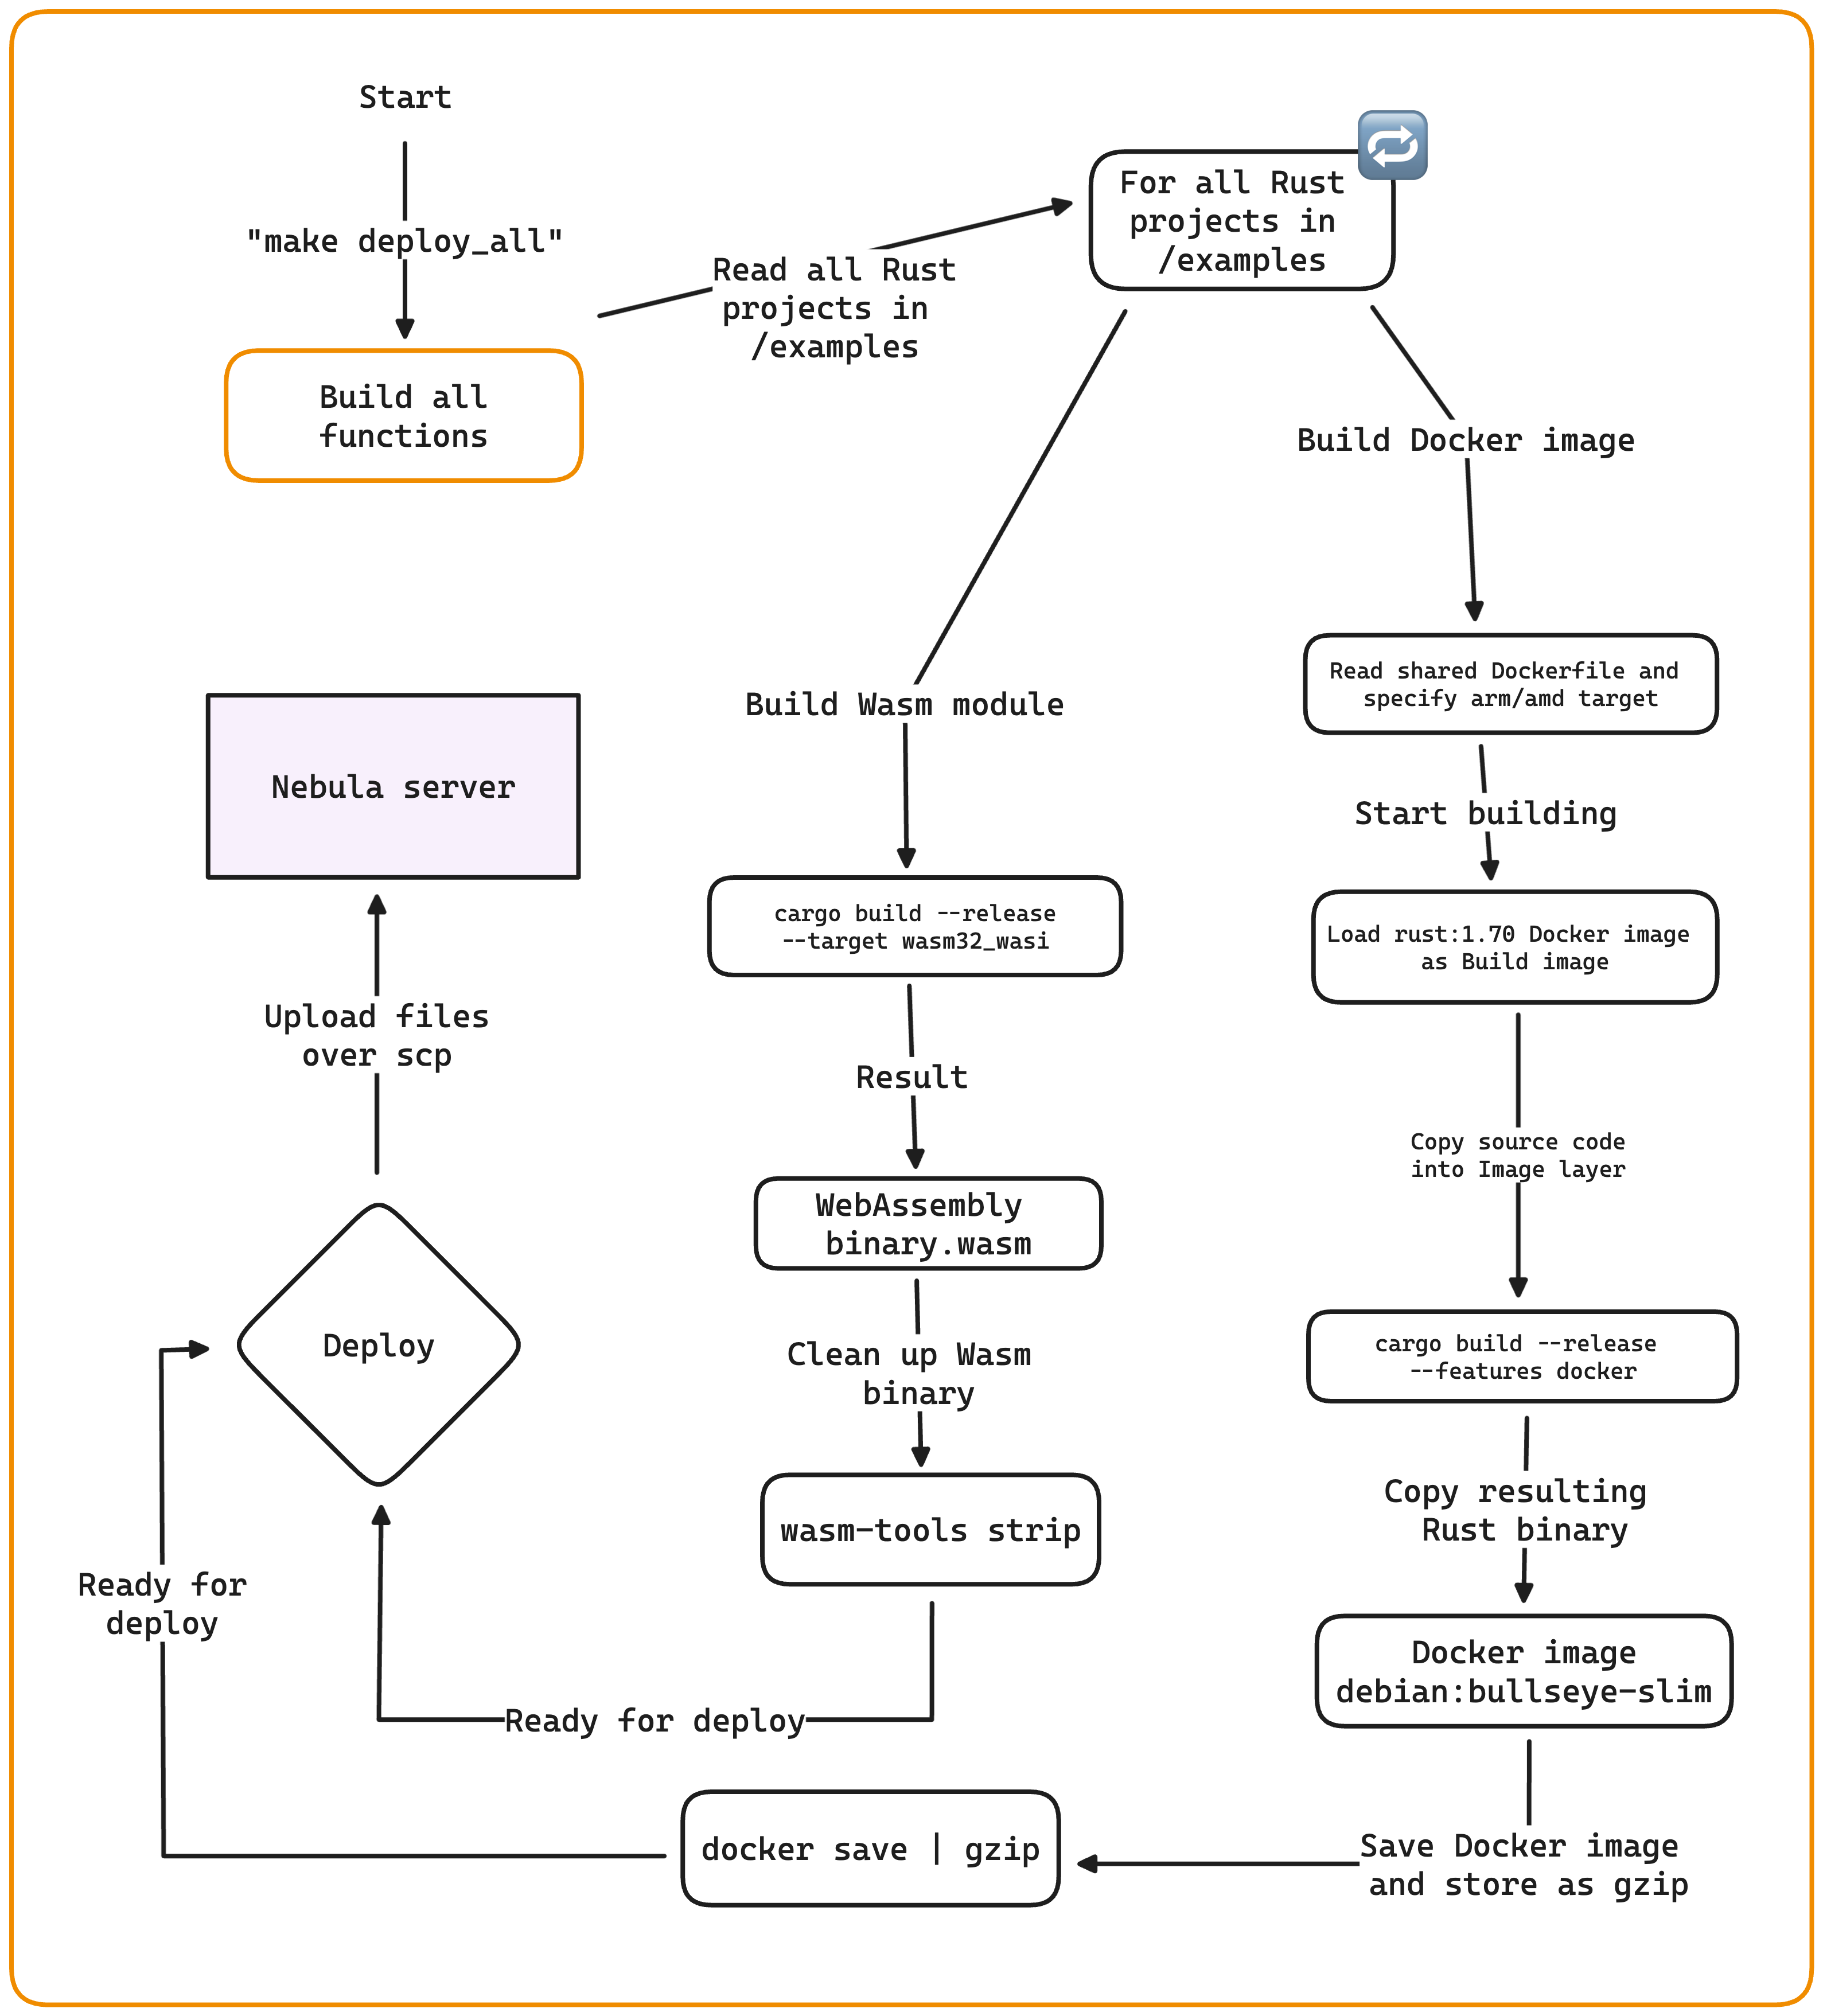
\includegraphics{assets/6-build_deploy_functions.png}
  \caption{Streamlined flow of building and deploying functions.}
  \label{fig:build_deploy_function}
\end{figure}

One thing to note in this flow, is the step \emph{wasm-tools strip}.
\emph{wasm-tools} is a CLI tool maintained by the Bytecode Alliance that
includes a series of tools we can use to manipulate our \ac{Wasm}
modules. Compiling a Rust program to \ac{Wasm} includes some unnecessary
sections that we can strip away. The \ac{Wasm} binaries we built for our
experiments resulted in \textasciitilde2Mb in size. Using this tool lets
us cut this down to \textasciitilde200Kb instead, while still
maintaining its function. More on that in our \Cref{chap:results}.

\subsection{Implementing a Benchmark Function}

Now that we have set up an environment for building and deploying
functions to Nebula, we can look at how we developed the benchmark
functions themselves. We will implement the recursive Fibonacci function
in this section.

\inputminted{rust}{assets/code/fib-recursive.rs}

Our shared library handles the core functionality. As described in
\Cref{sect:challenges}, we treat our functions as normal programs, which
we do by running them by invoking their main function. In this main
function we determine if the function will be compiled to a \ac{Wasm}
module or a Docker container based on the \texttt{-\/-features\ docker}
flag we pass in our build command. (See
\Cref{fig:build_deploy_function})

Then we implement the \texttt{fib} function which takes in what number
in the Fibonacci sequence we're interested in, which we have implemented
recursively, and pass this into our \texttt{run\_function} wrapper from
our shared library.

With that in place, we just need to set up our deployment targets - the
Raspberry Pi and the Debian-based virtual machine on \ac{NREC}.

\section{Deployment Setup}

For our research we have decided to set up Nebula both on a Raspberry Pi
running Debian on an ARM-based CPU, and on a virtual machine running on
\ac{NREC}, with gives us an AMD-based virtual CPU.

\subsection{Raspberry Pi Setup}

The Raspberry Pi, a low-cost and energy-efficient \ac{SBC}, was chosen
as one of our deployment targets to measure power consumption of our
function executions. The model we chose was the Raspberry Pi 4 Model B,
with 4GB of RAM, running the lite version of the Raspberry Pi OS, which
is built on top of Debian.

\subsubsection{Hardware Setup}

\begin{enumerate}
\def\labelenumi{\arabic{enumi}.}
\tightlist
\item
  Use the Raspberry Pi image tool for installing Raspberry Pi OS (lite,
  without desktop). Configure the OS with:
\item
  Wifi credentials, if not using ethernet.
\item
  SSH key, created with ssh-keygen, used to authenticate when connecting
  to device through SSH. This is also useful for uploading our files
  through scp.
\item
  Insert the microSD into the device and connect it to power, which
  boots it up.
\item
  If device connects to internet, it will be discoverable as
  \texttt{raspberrypi.local}, which can be used instead of its
  IP-address.
\end{enumerate}

\subsection{Virtual Machine Setup (\ac{NREC})}

For our experiments, we chose \ac{NREC} as our \ac{IaaS} platform for
hosting our virtual machine and benchmark a more typical deployment
environment. To use this service, we had to contact the administration
and verify that we were a student at the University of Oslo.

Once inside the \ac{NREC} platform, we can launch an instance of our
virtual machine, following their guide\todo{add guide?} for doing so.
For our experiments we chose the pre-configured flavor of
\texttt{m1.medium}, which gives us 1 virtual CPU, 4GB of RAM and 20GB
storage space. The virtual machine was built with the base image of
Debian 12. After this is set up, we can ssh into the server with a
ssh-key we provided during setup.

\begin{figure}[H]
\centering
  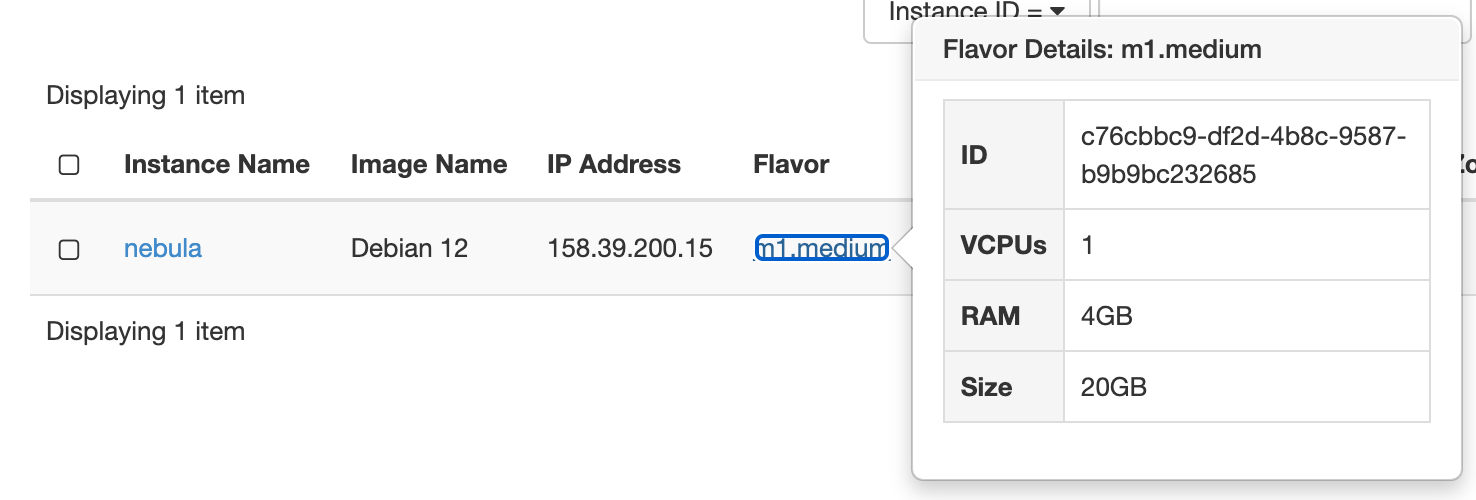
\includegraphics{assets/6-nrec_nebula}
  \caption{Our virtual machine configured on \ac{NREC}.}
  \label{fig:nrec_nebula}
\end{figure}

\subsection{Software Setup}

As both our setups are running a flavor of Debian, setting up the
software required to run our experiments are identical.

\begin{itemize}
\tightlist
\item
  First we update the package lists and upgrade pre-installed packages
  on our server:
\end{itemize}

\inputminted[firstline=12, lastline=13]{shell}{assets/code/commands.sh}

\begin{itemize}
\tightlist
\item
  Then we install Docker Engine following their official guide from
  their manual\footnote{\url{https://docs.docker.com/engine/install/debian/}}.
\end{itemize}

At this point, we are ready to deploy Nebula to each server and deploy
our functions.

\subsection{Tying It All Together}

Once we have install the required software on our servers, we can start
to deploy our Nebula web server and upload our \ac{Wasm} modules and
Docker images.

In our main project folder, we build Nebula using the cargo build
command. We add the flag \texttt{-\/-release}, which optimizes the
binary for production, and the flag
\texttt{-\/-target\ \textless{}target-arch\textgreater{}}, which
cross-compiles Nebula to the target architecture. Our prototype was
developed on a M2-based Macbook pro, so the default build target is not
supported on our target platforms. Cross-compiling works fine, but the
easiest and fastest way to build Nebula is to do it on the target
architecture itself.

For the Raspberry Pi, this was done by cloning the Github repository
with the source code onto the device, and building it from there. For
the \ac{NREC} implementation, a Github action was implemented for
building the application on a Linux VM as part of their CI/CD service.
This is not a crucial detail for our research, but valuable for anyone
who would want to recreate the experiment and expand upon it.

Finally, we build and deploy our functions as described in
\Cref{sect:shared_lib}, and upload our \ac{Wasm} binaries and our
gzipped Docker images to each server. Part of deploying the Docker
images is loading them into the local Docker image list, done with the
command \texttt{docker\ load\ -i\ /path/to/image.tar.gz}. When we start
our server we call the \texttt{serialize\_wasm()} function and serialize
our \ac{Wasm} modules into byte\_code that we can load and run on
Wasmtime. With all this in place, we can now perform our experiments.

\section{Benchmarking}
\label{sect:impl_bench}

Now that we have our Nebula \ac{FaaS} prototype up and running on both
our Raspberry Pi and virtual machine on \ac{NREC}, we can start
implementing the benchmarking utility that will be used to conduct the
experiments and collect our data. While there exist tools out there for
performing experiments like this, the setup we have implemented would be
difficult to cover with an already existing tool. Because of this, we
will develop a custom benchmark utility in Rust, which will let us
collect the data we're interested in.

For our experiments we will need to implement two core functionalities.
First, we need to implement a function that loops through a pre-defined
set of input values for each function and perform POST requests to
Nebula, storing the function results on our computer. We also need a
function for measuring power measurements while performing our POST
requests to Nebula on our Raspberry Pi.

\subsection{Stress-Testing Nebula}

To benchmark Nebula's cold starts and runtime efficiencies, we will need
to perform a range of POST requests with the intent of gathering a wide
range of data that we can compare later. For this we rely on the widely
used Rust crate, \texttt{reqwest}, a library for performing http
requests in Rust. The code for performing the request in itself is
omitted from this example, but the suite of functions and their
corresponding inputs we're testing with can be seen here:

\newpage

\inputminted{rust}{assets/code/request.rs}

For our benchmark functions, we have found a range of values that
through manual testing, that will give us a clear picture on how our
prototype performs when running functions as \ac{Wasm} modules or Docker
containers.

The steps we take in our stress-test function are:

\begin{enumerate}
\def\labelenumi{\arabic{enumi}.}
\tightlist
\item
  Define a list of modules that we are going to benchmark. For each
  function we have a tuple that consist of three values.

  \begin{itemize}
  \tightlist
  \item
    The name of the function.
  \item
    The amount of input values we want to test for each function.\\
  \item
    The factor we want to multiply our input values with, to cover a
    wider range of input values for our experiments.
  \end{itemize}
\item
  Loop through our list of functions.
\item
  For each function, loop through a range of \textless0,
  steps\textgreater.
\item
  Determine input value by multiplying current step with factor.
\item
  Perform each set of function and input 6 times. This is in order to
  gather a mean of each metric for our results later, to account for
  variance in our results.
\item
  Perform a function invocation for each function as both Wasm and
  Docker sequentially, then append result to the final result.
\item
  Return the list of results.
\end{enumerate}

The final result of this, is a long list of values that we store as
JSON, for further analysis.

An example of a function result from benchmarking on our Raspberry Pi
looks like this:

\inputminted{json}{assets/code/result_example.json}

Part of our metrics is the timings for microseconds since epoch for the
start and end of each function invocation, this is important for our
power measurements.

\subsection{Measuring Power}

For communicating with our Gude expert control over Modbus TCP, we are
going to use the \texttt{tokio-modbus} crate. This library will let us
write an interface against the device over our network.

As was presented in \Cref{sect:energy_background}, we saw how a client
and server communicates through Modbus TCP packets. In figure
\Cref{fig:modbus_tcp_packet} below, we zoom into this packet, as they
are important for our implementation for communicating with our Gude
power supply.

\begin{figure}[H]
\centering
  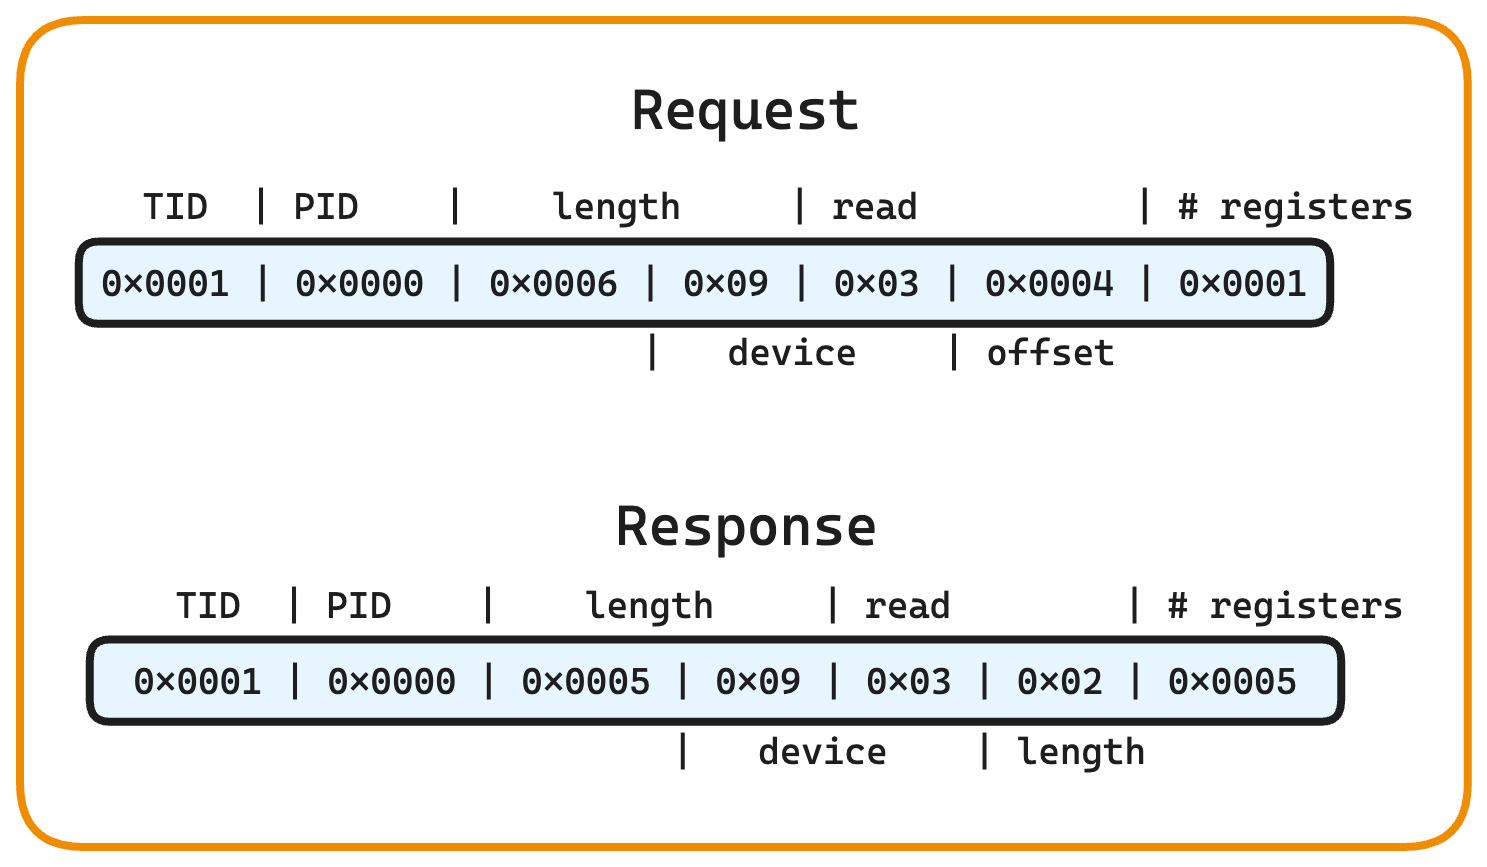
\includegraphics[width=0.7\columnwidth]{assets/6-modbus_packet.png}
  \caption{A Modbus TCP packet.}
  \label{fig:modbus_tcp_packet}
\end{figure}

To read from the packets we receive from our Gude power supply, we need
to know which register each measurement it can report to are registered.
From the manual of our Gude Expert Power Control 1105, we find this
table of sensor that it can report on. In \Cref{tab:gude_config} below,
we have extracted the most relevant sensors for our measurements, it's
register address, and how accurate it's reported units are.

\begin{table}[H]
\centering
\caption{\label{tab:unnamed-chunk-1}Gude Expert Power Control 1105 sensors. \label{tab:gude_config}}
\centering
\begin{tabular}[t]{ccrc}
\toprule
Offset & Sensor.Field & Address & Unit\\
\midrule
\cellcolor{gray!10}{0} & \cellcolor{gray!10}{Absolute Active Energy} & \cellcolor{gray!10}{0x400} & \cellcolor{gray!10}{Wh}\\
1 & Power Active & 0x402 & W\\
\cellcolor{gray!10}{2} & \cellcolor{gray!10}{Voltage} & \cellcolor{gray!10}{0x404} & \cellcolor{gray!10}{V}\\
3 & Current & 0x406 & mA\\
\cellcolor{gray!10}{4} & \cellcolor{gray!10}{Frequency} & \cellcolor{gray!10}{0x408} & \cellcolor{gray!10}{0.01hz}\\
\addlinespace
5 & Power Factor & 0x40a & 0.001\\
\bottomrule
\end{tabular}
\end{table}

As we can see from \Cref{tab:gude_config}, we can read Absolute Active
Energy, a value that is the cumulative sum of all energy consumed on our
device, measured in Wh. Power active reports the current W being drawn
at the moment of reading the sensor, the product of Voltage and Current.
At first glance, these two sensors seem ideal for our benchmarkings, but
as we will reveal in \Cref{chap:results}, the energy it takes to invoke
a function as either a \ac{Wasm} module or Docker container, will be
measured in μWh. Measurements in whole Watts will not provide accurate
enough data for our experiments. The three most important sensors for
our experiments will be Voltage, Current and Power Factor.

To re-iterate, the formula for calculating power is \(P = U \times I\),
where \emph{U} is voltage and \emph{I} is current. For example, with a
constant voltage of 240V and a current of 24mA, we will get
\(240V \times 24mA = 5,76mW\). Another important sensor to read from is
the Power factor, which is a factor that indicates how much power the
connected device is actually consuming, compared to the total draw of
current through the power cable. For our system it varied between 0.50
and 0.55, so with an example of \(PF = 0.55\) for our example above, we
get \(240V \times 24mA \times 0.55 = 3,168mW\). This product is what
we're going to collect data on.

In \Cref{sect:energy_challenges} we will discuss some challenges
regarding this setup, and most importantly that we are going to assume a
constant voltage of 240V for calculating our power measurements. This is
because for every sensor we want to read from our Gude device at a given
measurement adds up to the total amount of time it takes to read this
measure. When we limit our readings to focus on current and power
factor, our energy measurements come in fast enough to accurately time
them against our function executions.

\subsection{Reading from Modbus TCP}

For our sensor data, we are going to define a set of types and configure
a mapping of our sensor to register address data. For our measurements,
we will measure the current, power factor and time the start and end of
our readings. These timings will help us map power readings to the
function execution.

\inputminted[firstline = 33, lastline = 60]{rust}{assets/code/modbus.rs}

With this in place, and we can define our function for reading from
modbus. The goal of this function is to run in a parallell thread while
we conduct our stress-testing of Nebula on our Raspberry Pi. This
function will be run continually until the parent thread breaks, so we
will read measurements from Gude, described in code:

\inputminted[firstline = 0, lastline = 31]{rust}{assets/code/modbus.rs}

The steps we go through here are:

\begin{enumerate}
\def\labelenumi{\arabic{enumi}.}
\tightlist
\item
  Define our tcp client and connect it to our Gude device on the modbus
  tcp port (e.g., 192.168.68.71:502), and create an instance of our
  SensorData struct, where we set values to 0, and time the start of our
  measurement in microseconds since epoch.
\item
  Read current from its register, cast it as a floating point number and
  divide by 1000, so we get the value in \emph{A}, instead of \emph{mA}.
\item
  Read power factor from the register, which is multiplied by 1000 in
  the measurements, so we cast it to f32 and divide it by 1000 to get
  the power factor.
\item
  Calculate power at the time of measurement to \(240V \times I \times
  PF\) and return the power product and start and end times for the
  measurement.
\end{enumerate}

\subsection{Attaching Power Measurement to Function Invocations}

When we benchmark Nebula on our Raspberry Pi, we spawn two threads that
run in paralell, using the Tokio async runtime. One of these threads
performs out stress-test function from \Cref{sect:stress_test}, while
the other reads from our read\_modbus\_data function from
\Cref{sect:read_modbus}. We continue to read sensor data until the
stress-test function is completed, and save both lists as a variable.
Then we pass both the resulting function invocation results and the
power readings to a function that finds power measurements that coincide
with a function invocation.

\Cref{fig:power_measurement_timeline} below illustrates how power
measurements are paired with coinciding function invocations to estimate
the power required to run our functions.

\begin{figure}[H]
\centering
  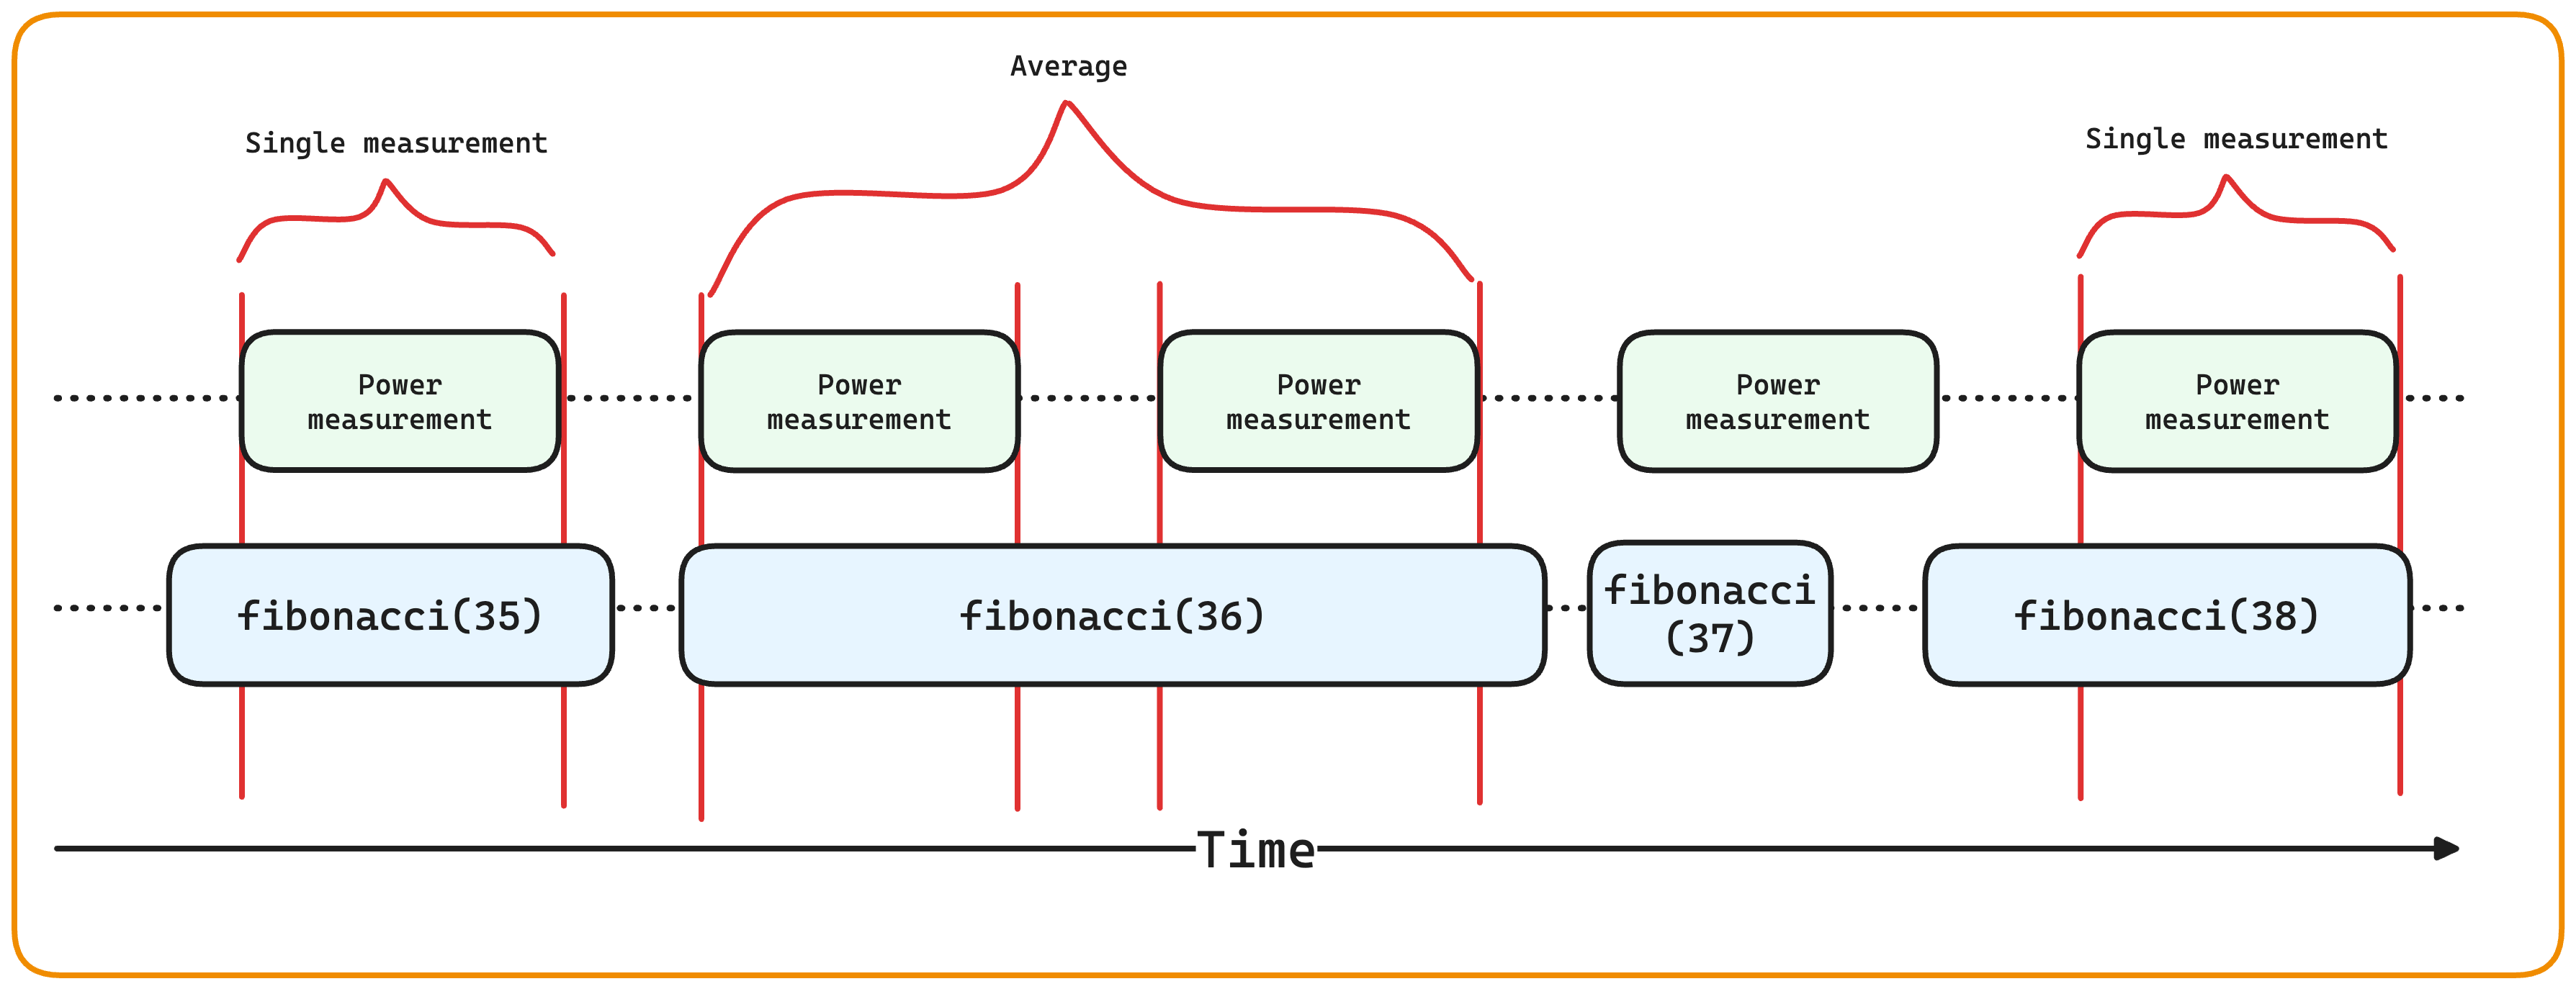
\includegraphics{assets/6-power_measurements}
  \caption{Power measurements that overlap with function invocations}
  \label{fig:power_measurement_timeline}
\end{figure}

In some of our benchmarks, there were instances of function invocations
being too fast to be able to pair with an power measurement. In these
cases, we ran the functions with its input multiple times, to ensure
that every input value for each function has the same amount of
invocations to improve the validity of our data. In other cases, we saw
functions that were so slow that multiple power measurements were
performed over the functions lifetime, and in this case we sum all the
corresponding measurements and get the average power consumption. For
example, a slow recursive fibonacci function might have 30 power
readings associated with it.

The code below shows how this is done. It loops through each function
result, finds the energy measurements that begin and end within the
start and end of each function invocation. Then it updates each function
result with the average power that was consumed by the system during the
functions execution. We also calculate the estimated \emph{Wh} in energy
consumption with the formula: \[P \times
\frac{t}{36000000000}\]

\inputminted{rust}{assets/code/pair_power_data.rs}

With this in place, we can now perform our experiments on both our
virtual machine and on the Raspberry Pi. \Cref{fig:physical_setup} below
shows the physical setup for the experiments on Nebula on our Raspberry
Pi.

\begin{figure}[H]
\centering
  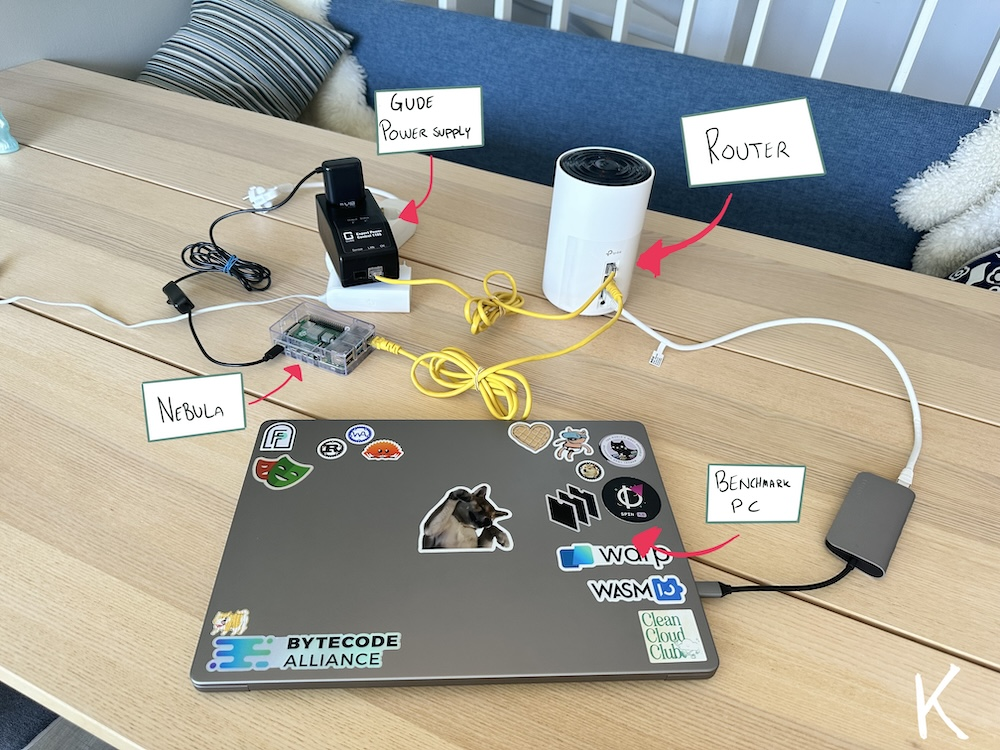
\includegraphics{assets/6-physical_setup.jpg}
  \caption{The physical setup, including the Raspberry Pi connected to power
through our Gude power supply. The Raspberry Pi and Gude controller is connected
to the benchmark computer on a local network through ethernet.}
  \label{fig:physical_setup}
\end{figure}

\subsection{Energy Measurement Challenges}
\label{sect:energy_challenges}

In \Cref{sect:energy_monitoring}, we saw several protocols and
measurement devices, and how they work, described. The first iteration
of measuring power was inspired by
\citet{qianEnergyFootprintingWordPress2022}, and consisted of an Aotec
Smart Switch 7, Aotec Z-stick 7 and relied on the zwave-js-ui
application to act as a publisher for reporting energy measurements over
\ac{MQTT}. This setup had one major flaw; energy reporting through
\ac{MQTT} could only be reported once every 30 seconds at a minimum.
This turned out to be too slow for attempting to measure accurate
readings for our experiments.

This limitation was unexpected, but Qian had used an Aotec Smart Switch
6, the previous generation, which turned out to support reporting once
every second. This device was luckily found on Finn.no, and allowed us
to upgrade the accuracy own to measuring every second instead.

However, as we will present in \Cref{chap:results}, our function
executions on our Raspberry Pi can come down to single-digit
milliseconds, meaning that once every second is still not accurate
enough to pinpoint the current draw on our system for each function
invocation.

The Gude Expert Power Control 1105 turned out to be the most suited
device for our experiments. This device supports many protocols, one of
which is the Modbus TCP protocol. By switching to this power supply,
connecting our Raspberry Pi and benchmarking computer to the same
network over ethernet, and changing the communcation method from
\ac{MQTT} to Modbus TCP, we were able to perform energy readings in
microseconds.

\section{Testing - Validity and Rigidity}

While formal unit testing was not exercised during the development of
Nebula, the choice of the Rust programming language provided inherent
benefits in terms of code reliability and correctness, ensuring the
validity and rigidity of the prototype.

\subsection{Rust's Compiler Guarantees}

As outlined in \Cref{sect:tech_stack}, chosing Rust as the programming
language was driven by its strong relationship with \ac{Wasm} and its
suitability for building efficient and scalable applications.
Significant factors to this are Rust's strict compiler checks and
emphasis on memory safety, concurrency, and parallelism. These factors
help

The Rust compiler enforces a set of rules that prevent common
programming errors, such as null pointer dereferences, data races, and
memory leaks. By catching these issues at compile-time, Rust eliminates
entire classes of runtime errors, increasing the overall stability and
predictability of the codebase.

Furthermore, Rust's ownership model and borrowing rules ensure safe and
efficient memory management, without the need for manual intervention or
a garbage collector. This approach reduces the risk of memory-related
bugs, which are very difficult to detect and resolve. We can't guarantee
that there are not any present in Nebula, as testing will never be able
to guarantee the absence of bugs. However, we saw that during extensive
stress-testing, our prototype consistently for several hours straight
during our benchmarks.

One exception to these guarantees is the deserialization of our
\ac{Wasm} modules, as discussed in \Cref{sect:6-challenge_insights}. In
this case, we opt out of Rust's compiler guarantees by telling the
compiler that we have a better understanding of the situation and can
safely read our \ac{Wasm} binary files as bytecode. While this
represents a potential risk if malicious binaries were to be introduced
to the web server, it did not pose an issue for our research.

\subsection{Rigorous Testing and Benchmarking}

Although formal unit testing was not a primary focus, the code underwent
rigorous manual testing and code review processes. As detailed in
\Cref{sect:impl_bench}, the components of Nebula were thoroughly tested
with various input scenarios, edge cases, and stress tests to ensure
correctness and robustness.

Moreover, the benchmarking suite itself, described in
\Cref{sect:impl_bench}, served as a form of integration testing,
exercising the entire system end-to-end and validating the correctness
of the results.

The combination of Rust's language features, idiomatic coding practices,
and extensive manual testing through the benchmarking suite provided a
strong foundation for the validity and rigidity of the Nebula prototype,
ensuring reliable and robust performance during the experiments and
evaluation.

\part{Analysis}

\newpage
\chapter{Results}

\setlength\epigraphwidth{.6\textwidth} 
\epigraph{\itshape  
One accurate measurement is worth a thousand expert opinions.
}{---Grace Hopper}

With the first goal of developing a prototype cloud computing platform
for the \ac{FaaS} paradigm accomplished, we can turn our attention to
the remaining objectives of this thesis. Leveraging the prototype
implemented in \Cref{chap:implement_nebula} and the supporting benchmark
utility, experiments were conducted on Nebula to evaluate its
performance. This chapter presents the results, while we will discuss
these results further in \Cref{chap:discussion}.

\section{Methodology Recap}

The experiments involved running a series of benchmark functions on both
a Raspberry Pi model 4B and a virtual machine on \ac{NREC}, representing
different operational environments. Each function was tested as a
\ac{Wasm} module and a Docker container to capture a comprehensive
dataset under controlled conditions. The key metrics measured were:

\begin{itemize}
\tightlist
\item
  Startup latency (Cold start): The time elapsed between invoking the
  function and its exeuction start.
\item
  Total runtime: The complete lifecycle duration from start to result
  return.
\item
  Power consumption: The power draw (in watts)on the Raspberry Pi during
  function execution loads, calculated as the product of measured
  current, power factor, and an assumed 240V voltage.
\end{itemize}

Additionally, by combining total runtime and power consumption data, an
estimation of the energy consumed by function executions throughout
their lifetime could be derived. Due to the fast execution times of our
functions, energy consumption (\emph{E}) is expressed in microwatt-hours
(μWh), calculated as \(E = P
\times t\), where P is the power in watts and t is the time in
microseconds.

To ensure accuracy and repeatability, data collection was automated
using the benchmarking utility developed in
\Cref{sect:implement_benchmark}, proving invaluable for this report.

Of particular note is the extreme performance disparity between
\ac{Wasm} modules and Docker containers, making it difficult to
visualize their data on the same graphs effectively. Consequently, where
applicable, the data is presented seperately to allow for closer
examination of each execution mode.

\section{Startup and Runtimes}

\begin{figure}[H]

{\centering 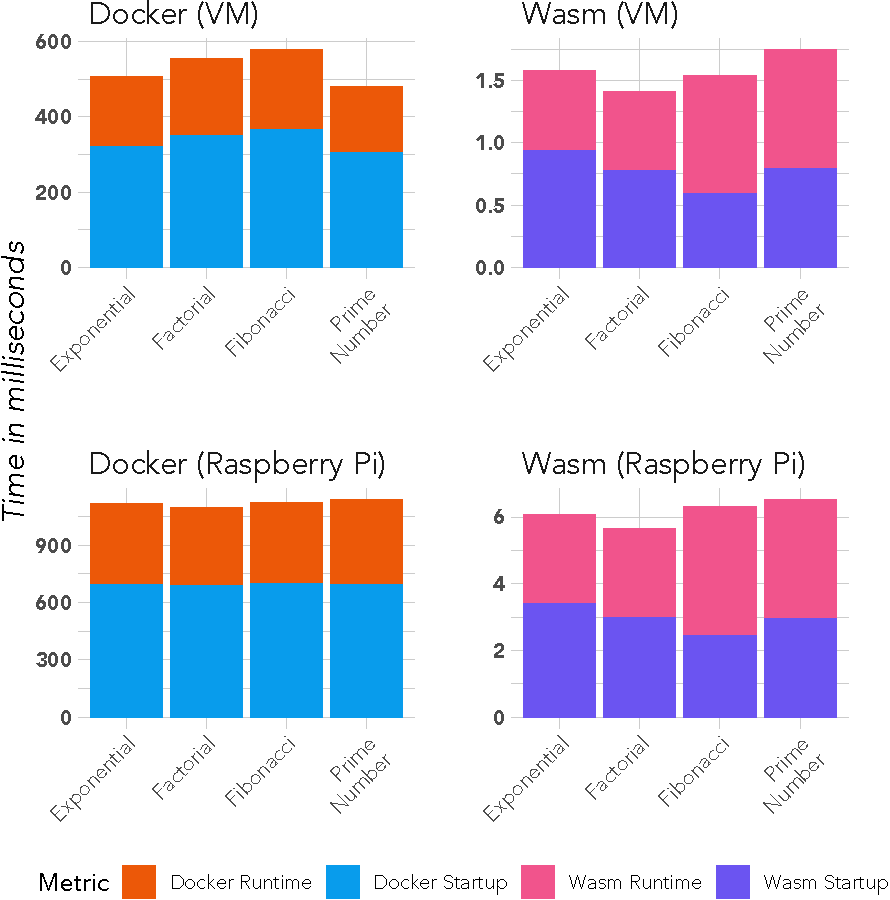
\includegraphics{thesis_files/figure-latex/avg-times-nrec-rpi-1} 

}

\caption{Average Startup and Runtime on both our setups}\label{fig:avg-times-nrec-rpi}
\end{figure}

\Cref{fig:avg-times-nrec-rpi} provides an overview of the average
startup and runtimes across our benchmarks on both our virtual machine
and Raspberry Pi setups. While this offers a general comparison between
\ac{Wasm} and Docker invocations,
\Cref{fig:nrec-efficiency, fig:rpi-efficiency} present more detailed
scatter plots with an average line drawn across showcasing the
performance variance for each input across multiple runs.

At first glance, the startup and runtimes of our \ac{Wasm} modules and
Docker containers may appear similar in \Cref{fig:avg-times-nrec-pi},
but a keen eye will notice the differeing y-axis scales. While Docker
containers startup and return results in the range of hundreds of
milliseconds, the \ac{Wasm} modules startup and shut down in just
single-digit milliseconds.

It is evident from these figures that the data follows a similar curve
on the Raspberry Pi, albeit with longer runtimes compared to the virtual
machine, as expected due to the resource constraintes of the former. To
account for variance, every permutation of function type, name and input
was executed at least five times during the benchmarking process.

For the sake of clarity, measurements exceeding specific input
thresholds for the fibonacci (above 30) and prime number (above 1500)
functions have been ecluded from the graphs, as their steep runtime
increases would impede effective visualization.

\newpage

\begin{figure}[H]

{\centering 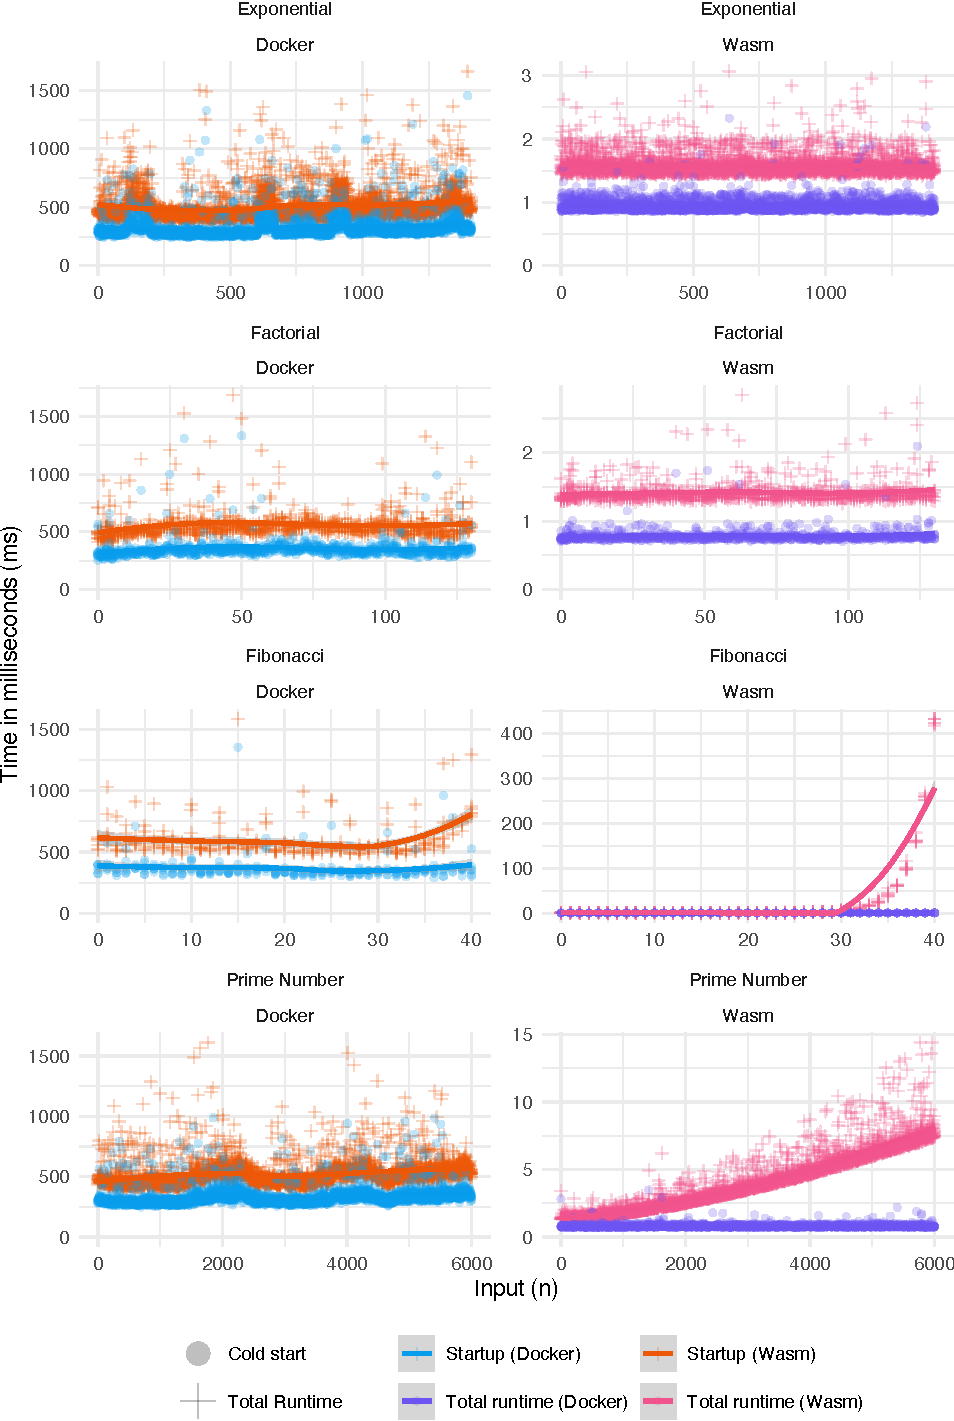
\includegraphics{thesis_files/figure-latex/nrec-efficiency-1} 

}

\caption{Wasm runtime measurements on VM during benchmarks.\label{nrec-efficiency}}\label{fig:nrec-efficiency}
\end{figure}

\newpage

\begin{figure}[H]

{\centering 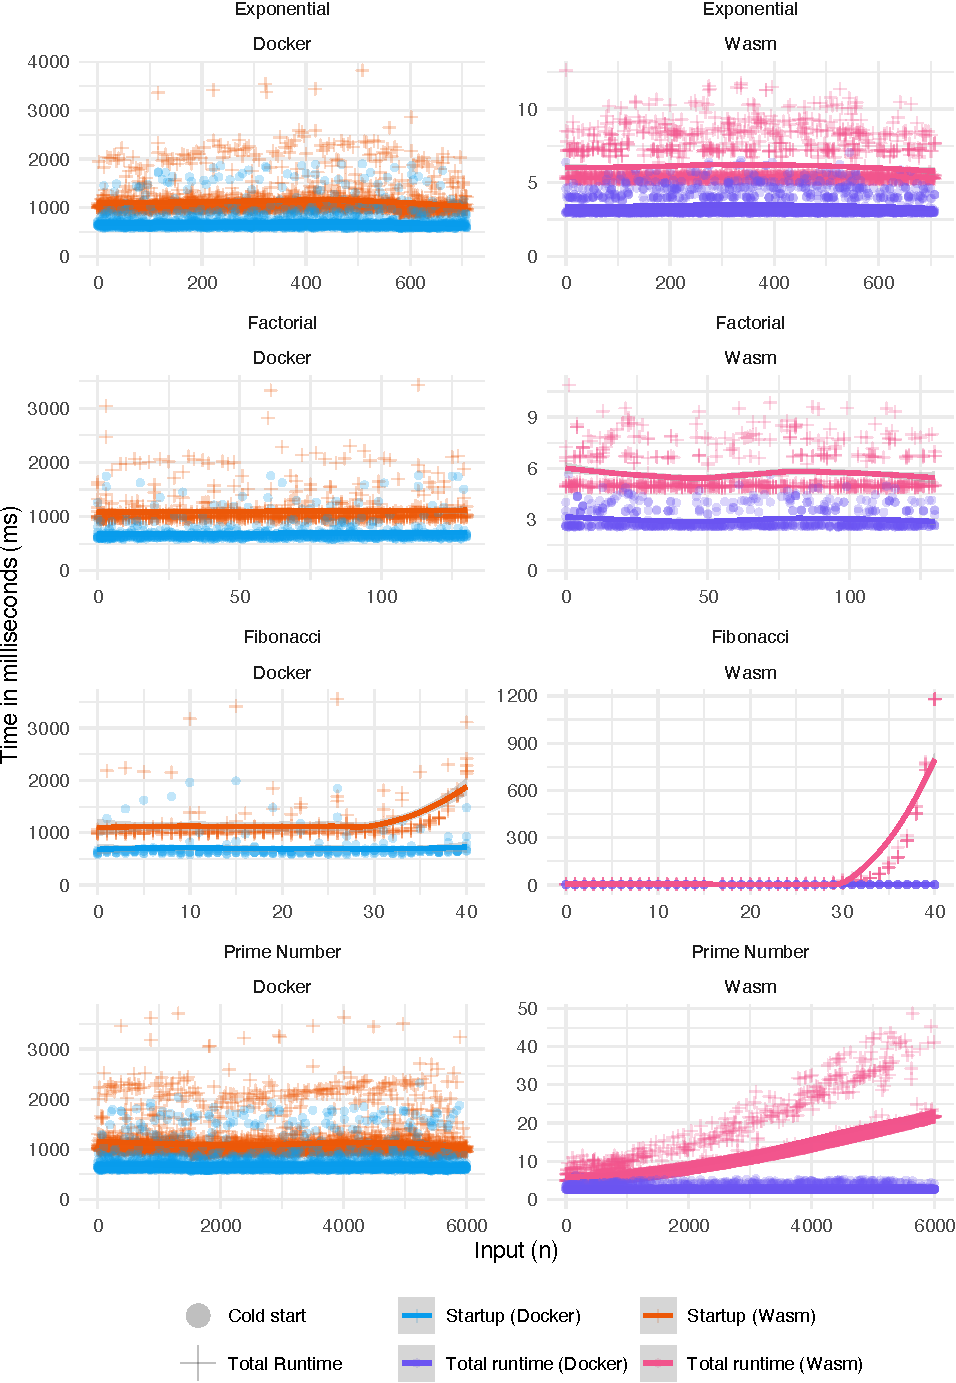
\includegraphics{thesis_files/figure-latex/rpi-efficiency-1} 

}

\caption{Startup and Runtime measurements on Raspberry Pi 4B during benchmarks.}\label{fig:rpi-efficiency}
\end{figure}

\newpage

\section{Power Load and Energy Consumption Results}

This section presents the data for power load and energy consumption
measured on the Raspberry Pi during our benchmarking experiments. The
results for each function are presented in pairs, with the first figure
of each pair showing the average power load in watts that the Raspberry
Pi drew during function invocations for each input value (\emph{n}). The
second figure displays the estimated energy consumed, in microwatt-hours
(μWh), calculated by multiplying the average power load by the total
execution time in microseconds for each function.

\todo{mention the average consumption chart below}

An interesting observation from the fibonacci and prime number functions
is that while the average power load converges to a constant value
beyond certain input for both \ac{Wasm} and Docker executions. Despite
the consistent power draw during prolonged execution times, the energy
consumption curves for each function type maintain their trajectories.

Despite the consistent power draw during prolonged execution times, the
energy consumed continues to increase along the same curve of each
execution mode. The divergence in energy consumption, even with
converging power loads, highlights the importance of considering both
power and time factors when optimizing energy efficiency in serverless
computing environments.

\begin{figure}[H]

{\centering 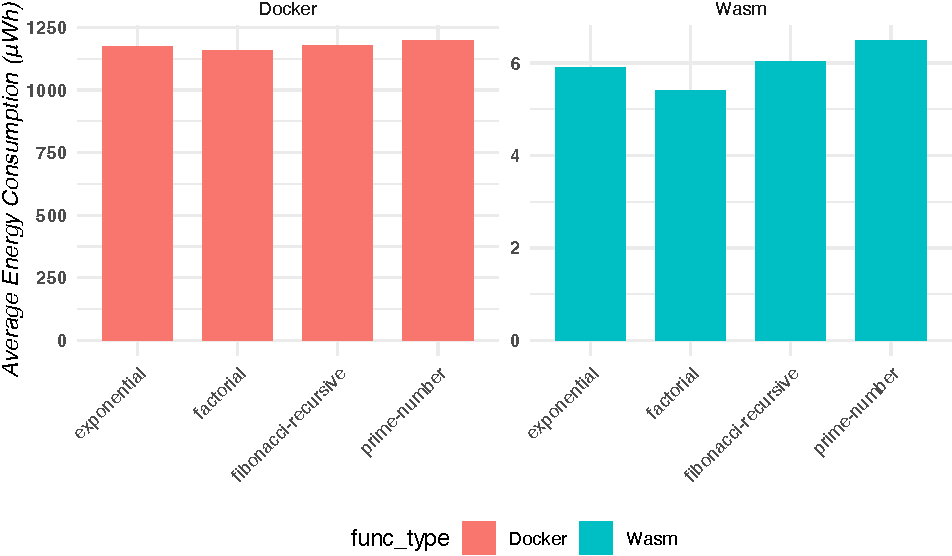
\includegraphics{thesis_files/figure-latex/avg-energy-consumption-rpi-1} 

}

\caption{Average energy consumption for our functions.}\label{fig:avg-energy-consumption-rpi}
\end{figure}

\begin{figure}[H]

{\centering 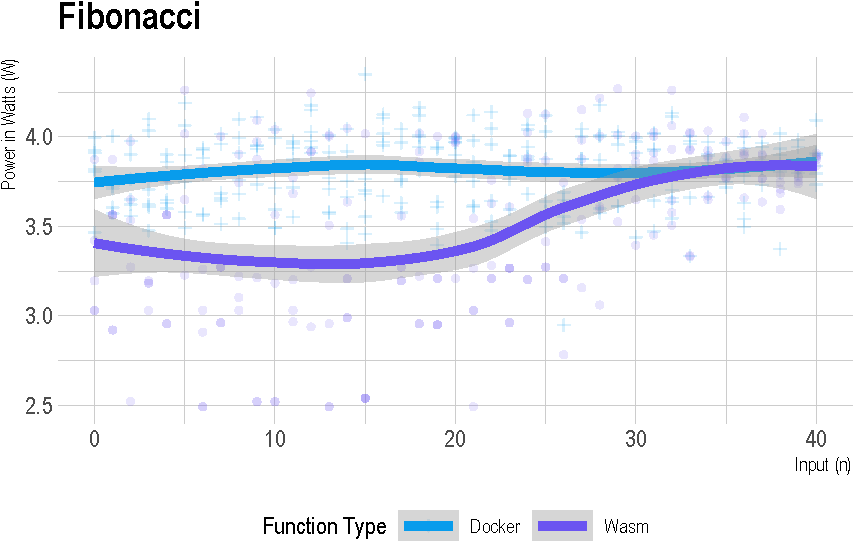
\includegraphics{thesis_files/figure-latex/fib-power-1} 

}

\caption{Power load on Raspberry Pi during Fibonacci benchmark.}\label{fig:fib-power}
\end{figure}

\begin{figure}[H]

{\centering 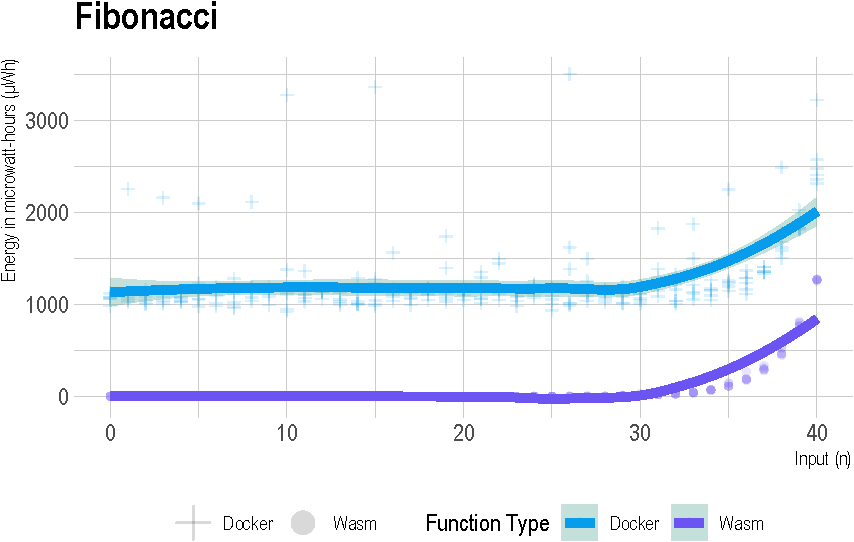
\includegraphics{thesis_files/figure-latex/fib-energy-1} 

}

\caption{Energy consumption on Raspberry Pi during Fibonacci benchmark}\label{fig:fib-energy}
\end{figure}

\newpage

\begin{figure}[H]

{\centering 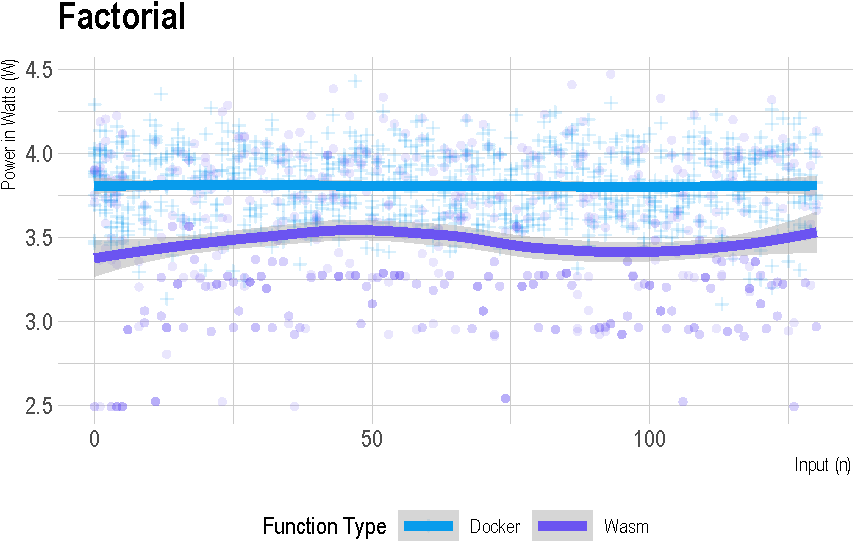
\includegraphics{thesis_files/figure-latex/fact-power-1} 

}

\caption{Power load on Raspberry Pi during Factorial benchmark.}\label{fig:fact-power}
\end{figure}

\begin{figure}[H]

{\centering 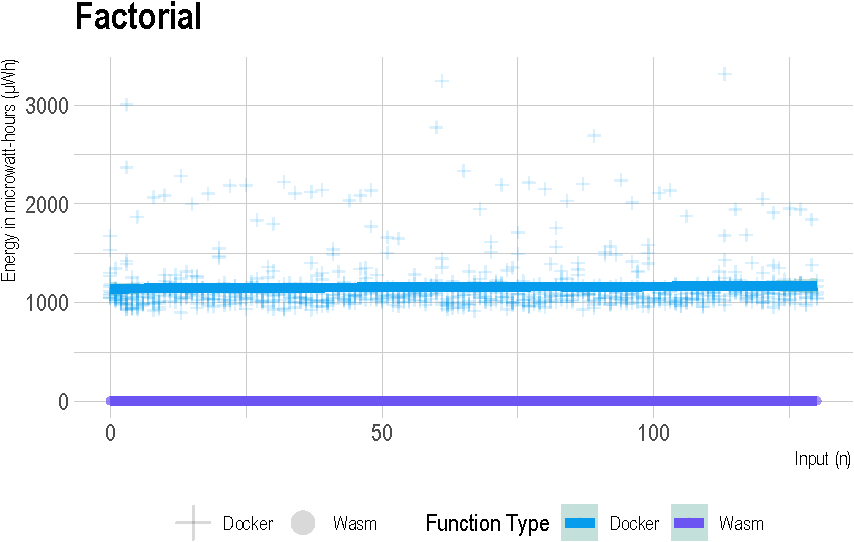
\includegraphics{thesis_files/figure-latex/fact-energy-1} 

}

\caption{Energy consumption on Raspberry Pi during Factorial benchmark.}\label{fig:fact-energy}
\end{figure}

\newpage

\begin{figure}[H]

{\centering 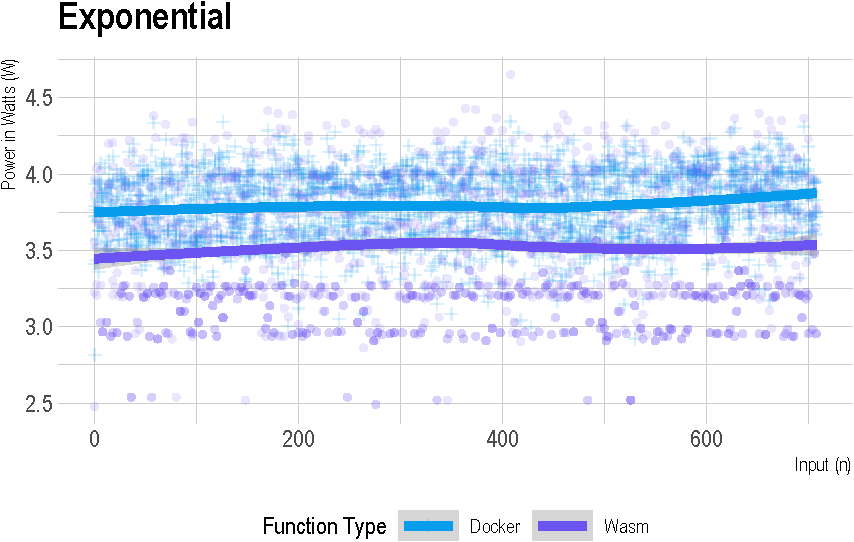
\includegraphics{thesis_files/figure-latex/exp-power-1} 

}

\caption{Power load on Raspberry Pi during Exponential benchmark.}\label{fig:exp-power}
\end{figure}

\begin{figure}[H]

{\centering 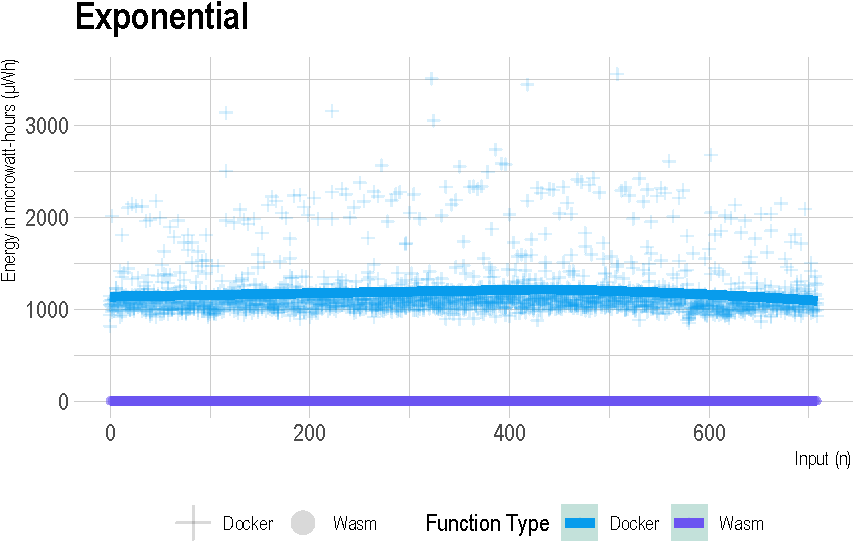
\includegraphics{thesis_files/figure-latex/exp-energy-1} 

}

\caption{Energy consumption on Raspberry Pi during Factorial benchmark.}\label{fig:exp-energy}
\end{figure}

\newpage

\begin{figure}[H]

{\centering 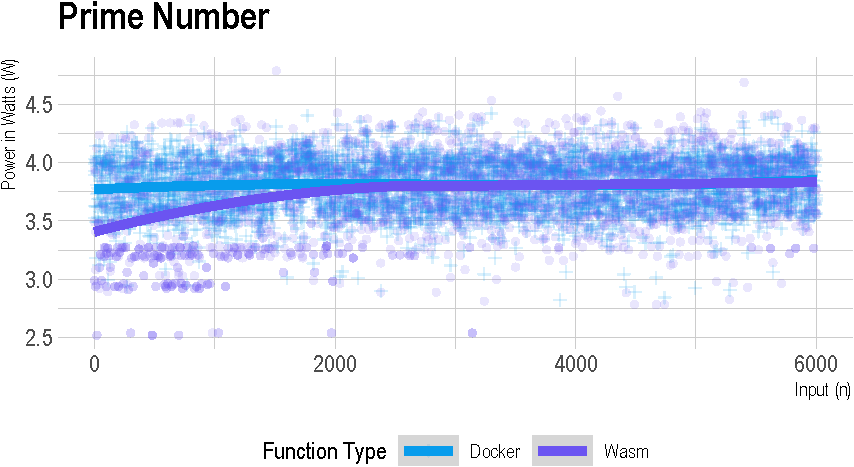
\includegraphics{thesis_files/figure-latex/prime-power-1} 

}

\caption{Power load on Raspberry Pi during Prime Number benchmark.}\label{fig:prime-power}
\end{figure}

\begin{figure}[H]

{\centering 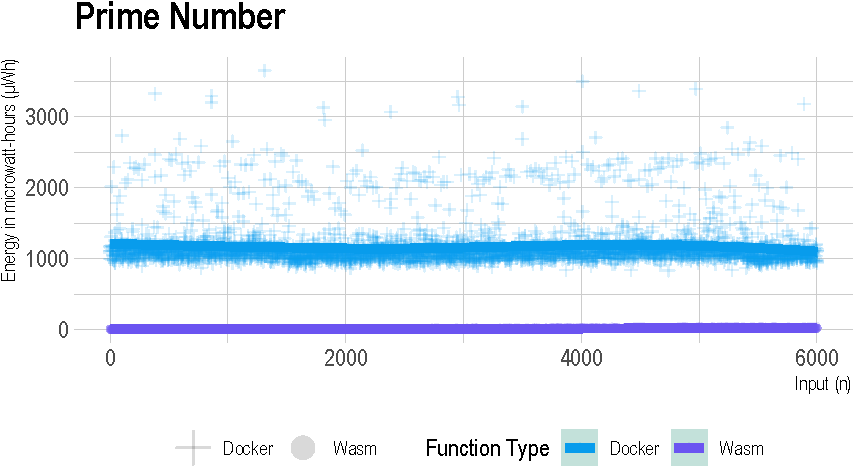
\includegraphics{thesis_files/figure-latex/prime-energy-1} 

}

\caption{Energy consumption on Raspberry Pi during Prime Number benchmark.}\label{fig:prime-energy}
\end{figure}

These results provide insights into the power and energy implications of
executing various functions as \ac{Wasm} modules and Docker containers
on resource-constrained devices like the Raspberry Pi. While this
controlled experiment does not necessarily accurately represent larger
data centers, the data can still inform decision-making processes
related to function deployment, resource allocation, and energy
optimization strategies in serverless computing environments.

\newpage
\chapter{Discussion}

The results obtained from our experiments shed light on the performance
characteristics and resource implications of serverless function
execution using \ac{Wasm} modules and traditional Docker containers. In
this chapter we will discuss the key findings, their significance and
compare them to existing research in this domain.

\section{Startup Latency and Runtime Performance}

Our experiments revealed a substantial difference in startup latency
between \ac{Wasm} modules and Docker containers. As illustrated in
\Cref{fig:avg-efficiency-nrec-rpi}, \ac{Wasm} function invocations on
average showed startup times approximately 365 times faster than their
Docker counterparts on the virtual machine setup. While the gap is
smaller on Raspberry Pi, due to its resource constraints, it is still
noticeable with \ac{Wasm} starting up 217 times faster than Docker
containers on average. In \Cref{fig:nrec-efficiency, fig:rpi-efficiency}
we can see the detailed startup times of our functions across both our
setups, and while the values can vary a lot across invocations, we can
see that the trend for a consistent startup time is consistent.

In addition to faster startup times, the results in
\Cref{fig:avg-efficiency-nrec-rpi} indicates that \ac{Wasm} modules
maintained a notable performance advantage over Docker containers in
form of overall runtime. On the virtual machine, \ac{Wasm} runtimes were
between 217 times faster than Docker runtimes, and finally 324 times
faster for the functions entire lifetime, from start to finish. On the
Raspberry Pi, \ac{Wasm} still showed significant runtime improvements
compared to Docker containers, spending 146 times less time calculating
the result, and 183 times less time for the functions lifetime.
\Cref{fig:nrec-efficiency, fig:rpi-efficiency} shows the total runtime
on both setups, including the startup times, and here we can see that
most of the time spent during execution of our functions is spent on
startup. The exception to this is in the case of our fibonacci and prime
number functions, where the total runtime consistently go beyond the
startup time at input numbers above 30 and 1500 respectively. This
indicates that the improved runtimes of our \ac{Wasm}-based functions as
an alternative to Docker diminishes at heavier workloads.

A very interesting observation that is made apparent from
\Cref{fig-avg-efficiency-nrec-rpi} is that our Docker containers perform
unexpectedly slow in runtime, compared to the runtime of the same code
executed as \ac{Wasm} modules. The ratio of our tuntimes across both
\ac{Wasm} and Docker remains largely the same, but with the same source
code, one could expect that the Rust binary inside the Docker container
would perform close to the same source code compiled to \ac{Wasm}.
Examining this discrepancy would be valuable to explore in future work.

\section{Power Consumption and Energy Efficiency}

Another important aspect explored in our study is the power consumption
and energy efficiency of \ac{Wasm} modules compared to Docker
containers. As depicted in \Cref{fig:fib-power} to
\cref{fig:prime-energy}, our results from the Raspberry Pi benchmarks
revealed that \ac{Wasm} function executions consumed approximately 198
times less energy, measured in microwatt-hours (μWh), than their Docker
counterparts for the same computational workload.

While the average power load during execution converged to a consistent
value for both \ac{Wasm} and Docker instances at higher input values,
the energy consumption curves maintained their trajectories. This
divergence highlights the importance of considering both power and time
factors when optimizing for energy efficiency in serverless computing
environments.

Important to note for our power and energy measurements is that this
form of measuring power on a system is inherently not able to paint an
accurate representation on how much power and energy our functions
consume in isolation. Thus the results presented in \Cref{chap:results}
represent a approximation of how much energy our Raspberry Pi as a whole
consumes while executing our functions, including its other functions.
For our experiments we disabled unnecessary components, such as wifi,
bluetooth, HDMI and other connectors that draw constant power. We could
measure a ``baseline'' power draw that our system draws while idle and
not executing any functions and subtract this from our measurements, but
this would also only result in a close approximation with mostly the
same graphs with lower numbers.

\section{Related Work}
\label{sect:related-work}

Our findings on the performance and efficiency advantages of \ac{Wasm}
align with and complement the existing body of research in this field.

\citet{shillakerFaasmLightweightIsolation2020a} introduced a novel
serverless runtime, which employs \ac{Wasm} based ``Faaslets'' for
software-fault isolation. Similar to our observations, they reported
that Faaslets achieved cold start times 538 times faster than
traditional container-based operators and occupied between 6.5 to 25
times less memory during operation (\Cref{tab:dockervsfaaslet}).

\begin{table}[H]
\centering
\caption{\label{tab:unnamed-chunk-3}Comparison of Faaslets vs. container cold starts. Reprinted with permission.\label{tab:dockervsfaaslet}}
\centering
\begin{tabular}[t]{lrrr}
\toprule
 & Docker & Faaslets & vs.Docker\\
\midrule
\cellcolor{gray!10}{Initialization} & \cellcolor{gray!10}{2.8 s} & \cellcolor{gray!10}{5.2 ms} & \cellcolor{gray!10}{538×}\\
CPU cycles & 251M & 1.4K & 179K×\\
\cellcolor{gray!10}{PSS memory} & \cellcolor{gray!10}{1.3 MB} & \cellcolor{gray!10}{200 KB} & \cellcolor{gray!10}{6.5×}\\
RSS memory & 5.0 MB & 200 KB & 25×\\
\cellcolor{gray!10}{Capacity} & \cellcolor{gray!10}{\textasciitilde{}8 K} & \cellcolor{gray!10}{\textasciitilde{}70 K} & \cellcolor{gray!10}{8×}\\
\bottomrule
\end{tabular}
\end{table}

Additionally, they demonstrated a 2x speed-up in machine learning model
training and doubled throughput for interference tasks while reducing
memory usage by 90\% compared to traditional containers with Knative
(\Cref{fig:wasm-faasm}).

\begin{figure}[H]
\centering
  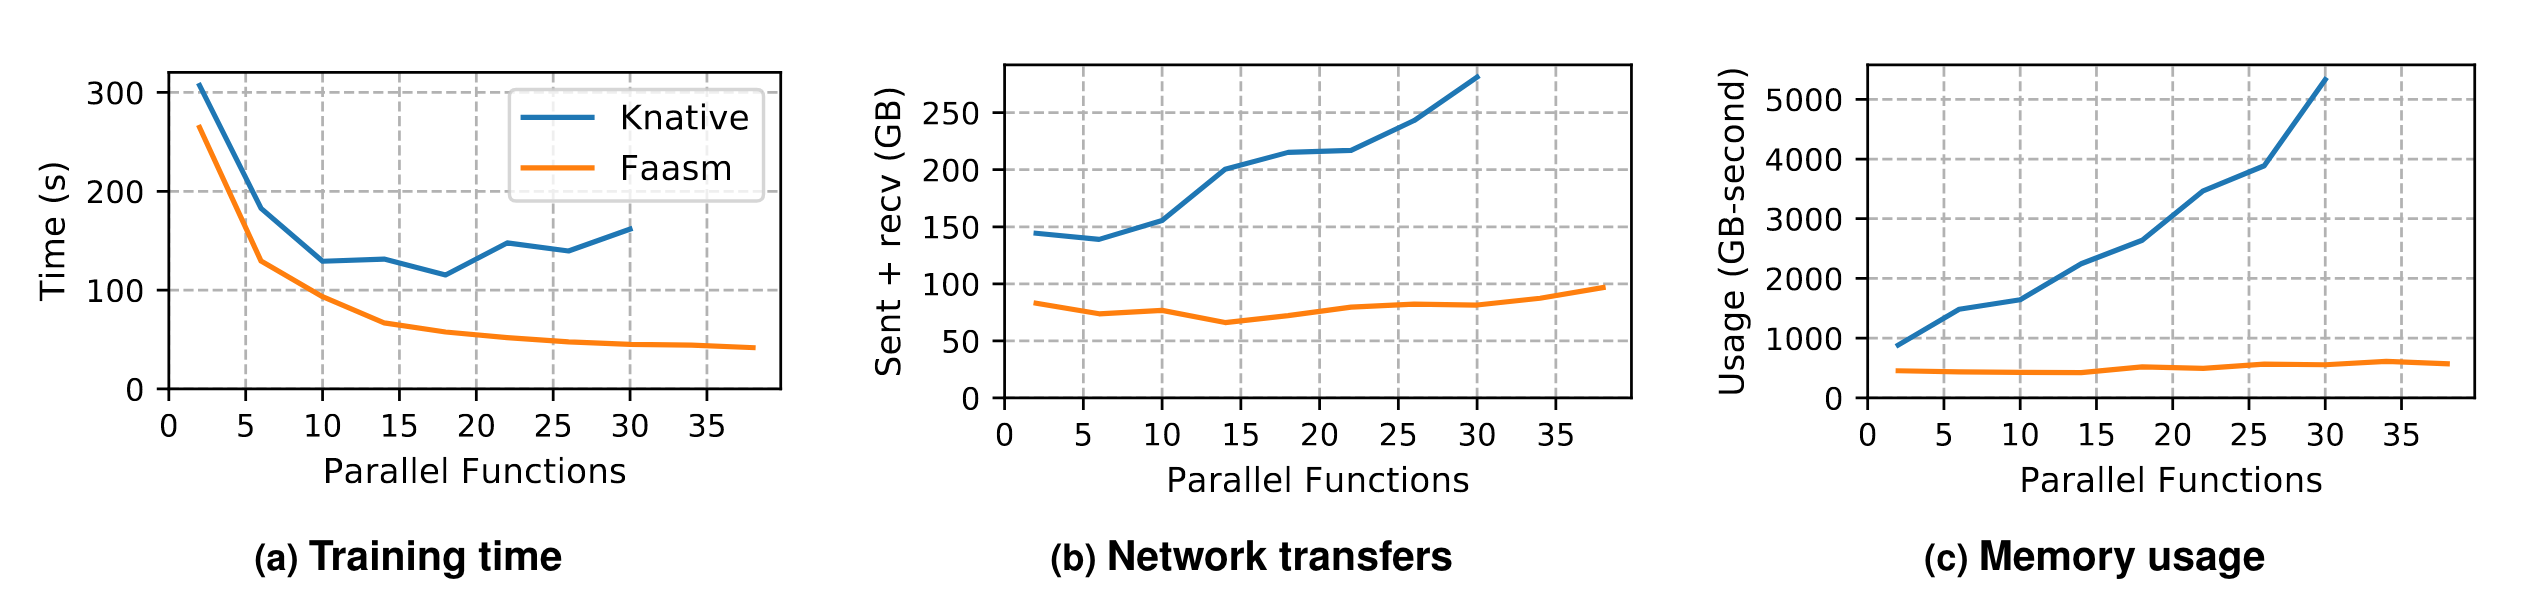
\includegraphics{assets/3.8-faasm.png}
  \caption{Machine learning training with SGD with Faaslets (FAASM) and containers (Knative). Reprinted with permission.}
  \label{fig:wasm-faasm}
\end{figure}

Our results indicating the drastic reduction in startup latency and
runtime improvements with \ac{Wasm} modules align closely with the
performance gains reported by
\citet{shillakerFaasmLightweightIsolation2020a}, further validating the
potential of \ac{Wasm} as a lightweight and efficient efficient
execution environment.

\citet{sebrechtsAdaptingKubernetesControllers2022} developed a
\ac{Wasm}-based framework for running lightweight controllers on
Kubernetes. They found that their \ac{Wasm}-based operators
significantly reduced memory footprint compared to traditional
container-based solutions. In their research they saw reductions from
1405MiB to 227MiB for 100 synthetic operators, and for idle operators
they saw a reduction from 1131MiB to 86MiB. (\Cref{fig:wasm-memory})

We didn't measure memory usage during our experiments, so the findings
of \citet{sebrechtsAdaptingKubernetesControllers2022} are not directly
appicable to our results, but their results corroborate with our
findings and show that \ac{Wasm} is a viable option on
resource-constrained setups.

\begin{figure}[H]
\centering
  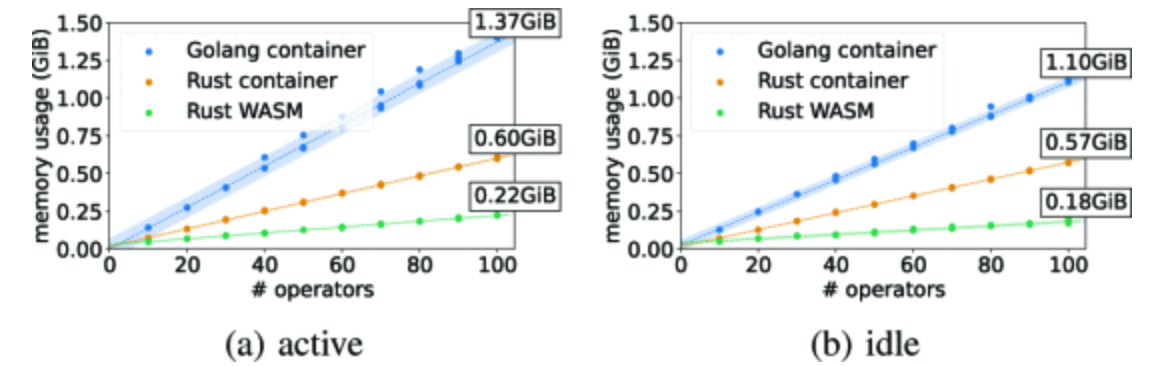
\includegraphics{assets/3.8-memoryusage-wasm.png}
  \caption{Different Kubernetes operators memory usage. Comparing Rust to WASM
vs Rust container vs Golang container. © 2022 IEEE}
  \label{fig:wasm-memory}
\end{figure}

\newpage
\chapter{Conclusion}

\epigraph{\itshape  
The more we got into WebAssembly, the more we thought, oh, this is actually a very, very powerful technology that can solve a wide variety of problems.
}{---Matt Butcher, \textit{CEO of Fermyon}}

With the first goal of this thesis achieved, we move our attention to
the topic of whether our hypothesis that Wasm offers a more efficient
alternative to Docker in regards to startup, runtime, and energy
consumption. Our findings are summiarised in
\Cref{tab:nrec-avg,tab:rpi-avg} which represent the differences in our
controlled experiments for this project.

\begin{table}[H]
\centering
\caption{\label{tab:nrec_data_table}Comparison of Wasm vs. Docker cold starts on VM.\label{tab:nrec-avg}}
\centering
\begin{tabular}[t]{llrr}
\toprule
  & Docker & Wasm & vs Docker\\
\midrule
\cellcolor{gray!10}{Cold start} & \cellcolor{gray!10}{324.66 ms} & \cellcolor{gray!10}{0.89 ms} & \cellcolor{gray!10}{365×}\\
Runtime & 187.03 ms & 0.69 ms & 271×\\
\cellcolor{gray!10}{Total runtime} & \cellcolor{gray!10}{511.69 ms} & \cellcolor{gray!10}{1.58 ms} & \cellcolor{gray!10}{324×}\\
\bottomrule
\end{tabular}
\end{table}

\begin{table}[H]
\centering
\caption{\label{tab:rpi_data_table}Comparison of Wasm vs. Docker cold starts on Raspberry Pi.\label{tab:rpi-avg}}
\centering
\begin{tabular}[t]{llrr}
\toprule
  & Docker & Wasm & vs Docker\\
\midrule
\cellcolor{gray!10}{Cold start} & \cellcolor{gray!10}{692.36 ms} & \cellcolor{gray!10}{3.19 ms} & \cellcolor{gray!10}{217×}\\
Runtime & 426.82 ms & 2.93 ms & 146×\\
\cellcolor{gray!10}{Total runtime} & \cellcolor{gray!10}{1119.18 ms} & \cellcolor{gray!10}{6.12 ms} & \cellcolor{gray!10}{183×}\\
Energy consumption & 1176.15 μWh & 5.95 μWh & 198×\\
\bottomrule
\end{tabular}
\end{table}

The findings from our experiments conclusively demonstrate the
superiority of \ac{Wasm} over Docker in terms of our scoped domain. As
evident from \Cref{tab:nrec-avg,tab:rpi-avg}, Wasm outperformed Docker
by significant margins across all aspects, including cold start times,
runtime, total runtime, and our estimation for energy consumption. It is
important to note that for certain computationally intensive functions
with very large input ranges (fibonacci-recursive with input
\textgreater{} 30 and prime-number with input \textgreater{} 1500). We
excluded those data points to avoid skewing the averages due to
excessive runtimes, like we did with figure
\Cref{fig:avg-efficiency-nrec-rpi}.

On the VM environment \Cref{tab:nrec-avg}, Wasm showed a remarkable 365×
faster cold start, 271× faster runtime, and 324× faster total runtime
compared to the same source code packaged into Docker images. Similarly,
on the Raspberry Pi \Cref{tab:rpi-avg}, Wasm showcased impressive
improvements, with 217× faster cold start, 146× faster runtime, 183×
faster total runtime, and 198× less energy consumed than Docker.

These findings underscore the potential of Wasm as a lightweight and
efficient execution environment for serverless functions, offering
significant performance benefits over traditional container-based
approaches. The drastic reduction in startup latency and runtime times
can be a serious advantage in scenarios where minimizing latency and
maximizing throughput are critical, such as in latency-sensitive
applications or high-throughput workloads. Furthermore, the significant
energy savings and the low memory usage
\citep{shillakerFaasmLightweightIsolation2020a} achieved by \ac{Wasm}
make it an attractive choice for resource-constrained environments, such
as edge computing devices or embedded systems.

While our experiments focused on specific workloads and environments,
the observed trends suggest that Wasm could be a viable and compelling
alternative to Docker for a wide range of serverless applications.
However, it is essential to note that the choice between Wasm and Docker
may also depend on other factors, such as the specific requirements of
the application, the available resources, and the trade-offs between
performance and other considerations, such as security and portability.

In summary, our research has demonstrated the potential of Wasm as a
high-performance and energy-efficient alternative to Docker for
serverless computing. The findings presented in this thesis provide a
solid foundation for further exploration and adoption of Wasm in the
serverless ecosystem, particularly in scenarios where performance,
latency, and energy efficiency are critical concerns.

\newpage
\chapter{Future work}

\setlength\epigraphwidth{.7\textwidth}

\epigraph{\itshape 
“So will wasm replace Docker?” No, but imagine a future where Docker runs linux
containers, windows containers and wasm containers side by side. Over time wasm
might become the most popular container type. Docker will love them all equally,
and run it all :)
}{---Solomon Hykes, \textit{Founder of Docker}}

While our findings sure are impressive, with \ac{Wasm} clearly coming
ahead in our controlled experiments in regards to the measurements we
set out to research, there is still a lot of room for exploring this
domain further. In essence, Nebula as a \ac{FaaS} platform is flawed.
For this project it was scoped down to focusing on pure functions, where
for every input we provide, we will always get the same output back.
This is fine for our controlled experiments, but the real world is not
that black or white.

\section{Investigating Docker Performance Discrepancies}

One intriguing observation from our results was the unexpectedly slow
runtime performance of the Docker containers compared to the \ac{Wasm}
modules, despite executing the same source code. This discrepancy
warrants further investigation to understand the underlying causes and
potential optimizations. Future work could involve a comprehensive
analysis of the Docker runtime environment inside the container. Factors
such as container initialization overhead, resource allocation
strategies, and potential bottlenecks in the exeuction pipeline would
prove very useful to improve the body of research.

\section{Distributed Deployment and Power Measurement}

While our experiments focused on evaluating Wasm modules and Docker
containers on individual devices, the serverless computing paradigm
often involves distributed deployments across multiple nodes. Future
research could explore the deployment of Nebula across a cluster of
devices, enabling the measurement of power consumption and energy
efficiency in a distributed setting. This would provide valuable
insights into the scalability and resource utilization of each
deployment approach in a more realistic serverless environment.

Due to the small size of each individual \ac{Wasm} module binary that we
observed in our implementation, there could be an interesting case of
exploring the idea of shipping the function code to the execution
environment. If the \ac{Wasm} binaries remain below 300Kb in size when
using tools like wasm-tools' strip feature, there could be cases where
it might be benificial to move the \ac{Wasm} binary closer to where the
request came from, instead of passing large bodies of JSON data across
the globe.

\section{Accurate Power Consumption Measurements}

The power consumption measurements obtained in this study, while
insightful, represent approximations of the overall system power draw
during function execution. To gain a more precise understanding of the
energy efficiency of Wasm modules and Docker containers, future work
could leverage advanced power measurement techniques. For example, the
recently released Raspberry Pi 5 incorporates internal systems for
measuring power consumption at a granular level, allowing for the
isolation of CPU and RAM power consumption from other components.
Additionally, Intel CPUs offer the RAPL (Running Average Power Limit)
feature, which could provide detailed insights into the power
consumption of specific hardware components during function execution.

By addressing these areas, future research can build upon the
foundations laid by this thesis, further advancing our understanding of
the performance and energy implications of Wasm modules in serverless
computing environments.

\chapter*{Acronyms}
\begin{acronym}
  \acro{IaaS}[IaaS]{Infrastructure-as-a-Service}
  \acro{FaaS}[FaaS]{Functions-as-a-Service}
  \acro{Wasm}[Wasm]{WebAssembly}
  \acro{WASI}[WASI]{WebAssembly System Interface}
  \acro{VMs}[VMs]{virtual machines}
  \acro{VM}[VM]{virtual machine}
  \acro{JVM}[VM]{Java Virtual Machine}
  \acro{NIST}[NIST]{National Institute of Standards and Technology}
  \acro{AWS}[AWS]{Amazon Web Services}
  \acro{GCP}[GCP]{Google Cloud Platform}
  \acro{ACI}[ACI]{Azure Container Instances}
  \acro{SBC}[SBC]{Single board computer}
  \acro{AOT}[AOT]{ahead-of-time}
  \acro{MQTT}[MQTT]{Message Queuing Telemetry Transport}
  \acro{NREC}[NREC]{Norwegian Reasearch and Education Cloud}
\end{acronym}

\chapter*{Appendices}

\printbibliography

\end{document}
